\documentclass[twoside,11pt,openright]{report}

\usepackage[utf8]{inputenc}
\usepackage[american]{babel}
\usepackage{a4}
\usepackage{hyperref}
\usepackage{natbib}
\usepackage{latexsym}
\usepackage{mathtools}
\usepackage{amssymb}
\usepackage{amsmath}
\usepackage{amsthm}
\usepackage{epsfig}
\usepackage[T1]{fontenc}
\usepackage{lmodern}
\usepackage[labeled]{multibib}
\usepackage{color}
\usepackage{xcolor}
\usepackage{datetime}
\usepackage{epstopdf} 
\usepackage{cleveref}
\usepackage{geometry}
\usepackage{tikz}
\usepackage[]{algorithm2e}
\usepackage{graphicx}
\usepackage{microtype}
\usepackage{varwidth}
\usepackage{subcaption}
\usepackage{pifont}

\SetAlFnt{\small}
\SetAlCapFnt{\large}
\SetAlCapNameFnt{\large}

\newcommand{\thesisurl}{\url{http://github.com/kasper0406/EditDistance}}

\graphicspath{ {../Benchmarks/} }

\renewcommand*\ttdefault{txtt}

\newcommand{\todo}[1]{{\color[rgb]{.5,0,0}\textbf{$\blacktriangleright$#1$\blacktriangleleft$}}}
\newcommand{\DIST}{\operatorname{DIST}}
\newcommand{\EditDist}{\operatorname{EditDist}}

\newcommand{\xfactor}{\ensuremath{\mathit{xfactor}}}
\newcommand{\ffactor}{\ensuremath{\mathit{ffactor}}}

\newcommand{\substr}[3]{#1\langle #2, #3 \rangle}
\newcommand{\str}[3]{#1[#2, #3]}
\newcommand*{\circled}[1]{\tikz[baseline=(char.base)]{
                          \node[shape=circle,draw,inner sep=2pt] (char) {#1};}}

\newcommand{\ceil}[1] {\lceil #1 \rceil}
\newcommand{\SLP}[1] {\mathcal{#1}}

\newcommand{\refbook}[2]{\cite[#1]{DBLP:journals/corr/abs-0707-3619}, #2}
\newcommand{\reftiskin}[2]{\cite[#1]{Tiskin:2010:FDM:1873601.1873704}, #2}

\newcites{A,B}{Primary Bibliography,Secondary Bibliography}

\newtheorem{mydef}{Definition}
\newtheorem{problem}{Problem}
\newtheorem{claim}{Claim}
\newtheorem{lemma}{Lemma}
\newtheorem{theorem}{Theorem}

% see http://imf.au.dk/system/latex/bog/

\crefname{algocfline}{algorithm}{algorithms}

\usetikzlibrary{shapes,arrows,positioning}
\usetikzlibrary{paths.ortho}

\begin{document}

\RestyleAlgo{boxruled}
\LinesNumbered

%%%%%%%%%%%%%%%%%%%%%%%%%%%%%%%%%%%%%%%%%%%%%%%%%%%%%%%%%%%%%%%%%%%%%%%

\pagestyle{empty} 
\pagenumbering{roman} 
\vspace*{\fill}\noindent{\rule{\linewidth}{1mm}\\[4ex]
{\Huge\sf Acceleration of Edit-Distance\\using Compression}\\[2ex]
{\huge\sf Kasper Nielsen, 20091182}\\[2ex]
\noindent\rule{\linewidth}{1mm}\\[4ex]
\noindent{\Large\sf Master's Thesis, Computer Science\\[1ex] 
\monthname\ \the\year  \\[1ex] Advisor: Christian Nørgaard Storm Pedersen\\[5ex]
\Large\sf \thesisurl\\[15ex]}\\[\fill]}

\epsfig{file=logo.eps}\clearpage

%%%%%%%%%%%%%%%%%%%%%%%%%%%%%%%%%%%%%%%%%%%%%%%%%%%%%%%%%%%%%%%%%%%%%%%

\pagestyle{plain}

\chapter*{Abstract}
\addcontentsline{toc}{chapter}{Abstract}
\begingroup
\let\cleardoublepage\clearpage

This thesis examines how and if computation of edit distance can be accelerated by means of a specific type of string compression.

Edit distance is a measure of the similarity between two strings and has applications including automatic spelling correction and DNA/Protein alignment. A well known dynamic-programming algorithm by Wagner and Fischer, in this thesis known as the simple algorithm, exists for computing the edit distance between two input strings.

The thesis is based on the algorithm described in \cite{Gawrychowski:2012:FAC:2422024.2422048} which is the latest paper in an ongoing refinement process of the algorithm. The objective of the thesis is to give a coherent description of the algorithm, prove that it works and implement and benchmark the algorithm to examine its practical feasibility.

The string compression method used, converts the input string into a restricted form of a context free grammar called a straight-line program (SLP). By utilizing a succinct representations of intermediate structures in the algorithm, it is possible to gain a theoretical speedup for compressible input.

In practice it was found that the compression based algorithm is only faster for highly repetitive input (for example Fibonacci strings and strings from a singleton alphabet) of length longer than $\approx 30000$ characters. For all other inputs the simple edit distance algorithm performed better. Therefore the compression based algorithm of \cite{Gawrychowski:2012:FAC:2422024.2422048}, in its current state, is not found to be favourable in any real-world practical problems.

\chapter*{Resum\'e}
\addcontentsline{toc}{chapter}{Resum\'e}

Dette speciale undersøger hvordan og om det er muligt at accelerere udregningen af edit distance ved at komprimere inputtet til algoritmen.

Edit distance er et mål for ensheden mellem to strenge og har anvendelser indenfor bl.a. automatisk stavekontrol samt DNA/Protein alignment. edit distance målet kan beregnes af en velkendt dynamisk-programmerings algoritme givet af Wagner og Fischer. Denne algoritme omtales i dette speciale som den simple algoritme.

Specialet er baseret på algoritmen beskrevet i \cite{Gawrychowski:2012:FAC:2422024.2422048}, som er det senest offentliggjorte resultat i en løbende raffinering af algoritmen. Målet med specialet er at give en sammenhængende beskrivelse af algoritmen, bevise at fremgangsmåden virker samt at implementerer og teste algoritmens opførsel i praksis.

Streng-komprimeringsmetoden der benyttes er en restringeret form for kontekstfri grammatik kaldet et straight-line program (SLP). Ved at bruge en koncis representation af de interne strukturer i algoritmen, er det muligt at opnå en teoretisk hastighedsforbedring for edit distance udregningen på komprimerbare inputs.

I praksis blev det fundet, at den komprimerings basered algoritme kun er hurtigere ved meget repetitivt input (for eksempel Fibonacci strenge eller strenge fra et singleton alfabet) med længde større end $\approx 30000$ tegn. For alle andre inputs blev det fundet at den simple algoritme præsterede bedre. Derfor er den komprimeringsbasered edit distance algoritme fra \cite{Gawrychowski:2012:FAC:2422024.2422048}, i dens nuværende form, ikke et foretrukket alternativ for nogen praktiske problemer i den virkelige verden.

\endgroup

% \chapter*{Acknowledgements}
% \addcontentsline{toc}{chapter}{Acknowledgments}

% \todo{\dots}

% \vspace{2ex}
% \begin{flushright}
%   \emph{Kasper Nielsen,}\\
%   \emph{Aarhus, \today.}
% \end{flushright}

\tableofcontents
\clearpage
\pagenumbering{arabic}
\setcounter{secnumdepth}{2}

%%%%%%%%%%%%%%%%%%%%%%%%%%%%%%%%%%%%%%%%%%%%%%%%%%%%%%%%%%%%%%%%%%%%%%%

\chapter{Introduction}
\label{ch:intro}
Edit distance is a measure of how similar or dissimilar two strings are. The edit distance measure is used in a wide range of practical problems, including automatic spelling correction and DNA/Protein alignment. This thesis will examine if compressing the input strings to straight-line programs (SLPs, see \cref{def:slp}) can speed up the edit distance computation.

The main focus of this thesis is based on the algorithm described in \cite{Gawrychowski:2012:FAC:2422024.2422048} which builds on top of the approaches described in \cite{DBLP:journals/corr/abs-1004-1194} and \cite{DBLP:journals/corr/abs-0707-3619}. To this date, this is the asymptotically best known algorithm in the RAM model for computation of edit distance in strings encoded by SLPs. Given two input strings $A$ and $B$ of length respectively $k$ and $l$, the algorithm runs in time $O(n N \sqrt{\log{\frac{N}{n}}})$, where $N = k + l$ and $n$ is the sum of sizes of the compressed strings (a formal definition on how $n$ is measured is given in \cref{ch:compressing-strings}). It is an open problem if the running time can be reduced to $O(nN)$. This is discussed further in \cref{sec:conclusion:future-work}.

This thesis has a two-fold objective. First and foremost to implement the algorithm and benchmark it to see how the technique performs in practice. The second objective is to give a coherent description of the algorithm and argue that it is correct. The proofs in order to establish the correctness follow the ones presented in \cite{DBLP:journals/corr/abs-0707-3619}, \cite{Gawrychowski:2012:FAC:2422024.2422048} and \cite{Tiskin:2010:FDM:1873601.1873704}. The proofs supplied in this report are in many cases more thorough, detailed and is a bit closer to the actual implementation.

The algorithm for speeding up the edit distance computation using compressed strings, can be divided into two major steps. The first is compressing the input strings, which is described in \cref{ch:compressing-strings} and the second step is the actual edit distance computation which uses the compressed strings as input. The algorithm for the actual computation is described in \cref{ch:algorithm}.

Both of the chapters are finished by presenting benchmarks. The benchmark section of \cref{ch:compressing-strings} describes how well different types of strings compress and verifies the theoretical running time of the compression algorithm. Especially the compressibility of different types of input is of great interest since it bounds the speedup of the computation. The benchmark section of \cref{ch:algorithm} verifies the theoretical running time of the algorithm, compares how well the compression based algorithm performs to a simple edit distance algorithm and lastly examines the time usage by the different steps (see \cref{sec:edit-dist-on-slps-steps}) of the compression based algorithm.

\paragraph{}
All code, raw measurement data, plots and referred literature used in this thesis can be found at \thesisurl. A description of the structure of the code is also supplied on the website, together with a short description of how to build and run the code.

\section{Overview}
This section is intended to give an overview of the implemented algorithms, how the proofs of correctness relate.

The main steps of the implemented algorithm based on string compression are the following:
\begin{itemize}
  \item Compress the input strings $A$ and $B$ to straight-line programs (SLPs) (defined in \cref{def:slp}).
  \item Divide the input strings into blocks of a certain size based on their SLP representation.
  \item Compute a structure called a DIST repository. This is a structure that for every pair of blocks in the two SLPs contains what is known as a DIST table. A DIST table is a representation of how the two blocks compares wrt. the computation.
  \item Compute the actual result by utilizing the DIST repository.
\end{itemize}
In order to gain a speedup the DIST repository is represented using a succinct representation. The concrete representation will be discussed in much more detail in \cref{ch:algorithm}. For now it is sufficient to know that the representation is based on a special class of matrices called simple unit-Monge matrices. It will be seen later that this representation facilitates both fast construction and usage of the DIST repository.

The algorithm relies on the following list of sub-algorithms which all have been implemented as part of writing this thesis:
\begin{itemize}
  \item The SLP construction algorithm of \cite{Rytter2003211}. Described in \cref{ch:compressing-strings}.
  \item Algorithm from \cite{DBLP:journals/corr/abs-1004-1194} for dividing the input strings into blocks of size $O(x)$ for some $x$, corresponding to productions in the SLP. Described in \cref{sec:algorithm:select-productions}.
  \item Algorithm from \cite{DBLP:journals/corr/abs-1004-1194} for building the DIST repository based on the blocks of the input string. Described in \cref{sec:algorithm:building-DISTs-overview}.
    \begin{itemize}
      \item This algorithm requires the ability to compute the minimum distance product (see \cref{def:minimum-distance-product}) of two simple unit-Monge matrices (see \cref{def:simple} and \cref{def:unit-monge}) given by \cite{Tiskin:2010:FDM:1873601.1873704}. Described in \cref{sec:algorithm:min-mult-two-unit-monge}.
    \end{itemize}
  \item Algorithm for computing the actual result by using the DIST repository. This algorithm is only superficially described in \cite{Gawrychowski:2012:FAC:2422024.2422048} and \cite{DBLP:journals/corr/abs-0707-3619}. \Cref{sec:algorithm:filling-grid-overview} describes the details of this computation. The algorithm relies on:
    \begin{itemize}
      \item An algorithm from \cite{Gawrychowski:2012:FAC:2422024.2422048} for computing the maximum distance product of a DIST table with an arbitrary vector. Described in \cref{sec:algorithm:max-mult-H-table-with-vector}.
      \item The maximum distance product algorithm further relies on an interval union find data-structure from \cite{Itai06lineartime}. Described in \cref{sec:algorithm:interval-union-find}.
    \end{itemize}
\end{itemize}
The algorithm for constructing the SLP representation of the input strings requires a suffix tree. In order to have a succinct and efficient suffix tree, a third party suffix tree implementation from the Succinct Data Structure Library (SDSL) \cite{SDSL} based on \cite{OHL:FIS:GOG:2010} is used.

In order to understand and prove the correctness of the algorithm a collection of proofs is described. \Cref{fig:proof-overview} gives an overview of how the main definitions, lemmas and theorems of this thesis relate. Also the figure points to the origin in the literature and is color coded by how much detail is added in this thesis compared to the literature.

\setlength{\tabcolsep}{3pt}
\tikzstyle{block} = [draw, rectangle, align=left, text width=3.5cm]
\newcommand{\nodecontent}[3]{%
  \parbox{3.5cm}{%
    \begin{tabular}{l p{2.2cm}}
      \multicolumn{2}{p{3.3cm}}{#1} \\
      \textit{Reference:} & #2 \\
      \textit{Literature:} & #3 \\
    \end{tabular}
  }%
}%
\newcommand{\coloredbox}[1] {\item[\mbox{\ooalign{\color{#1}\ding{110}\cr\hidewidth\color{black}$\square$\hidewidth\cr}}]}%

\begin{figure}[!htb]
  \centering
  \begin{tikzpicture}[font=\tiny\sffamily,node distance=4.2cm]
    \node[block,fill=white!90!green](simple-classification){
      \nodecontent{Characterization of simple matrices}
                  {\Cref{claim:simple-matrix-characterization}}
                  {\cite[p. 1288]{Tiskin:2010:FDM:1873601.1873704}}
    };

    \node[block,fill=white!90!cyan, right of=simple-classification](unit-Monge-classification){
      \nodecontent{Characterization of unit-Monge matrices}
                  {\Cref{lemma:unit-monge-characterization}}
                  {\cite[Lemma 2.11, p. 10]{DBLP:journals/corr/abs-0707-3619}}
    };

    \node[block,fill=white!90!green, below=1cm of simple-classification](DIST-H-table-relation){
      \nodecontent{Relating $\DIST$-tables and $H$-tables}
                  {\Cref{lemma:dist-H-relation}}
                  {\cite[p. 48]{DBLP:journals/corr/abs-0707-3619}}
    };

    \node[block,fill=white!90!yellow, right of=DIST-H-table-relation](dist-representation){
      \nodecontent{Succinct DIST representation}
                  {\Cref{lemma:H-permutation-representation}}
                  {\cite[Theorem 4.10, p. 49]{DBLP:journals/corr/abs-0707-3619}}
    };

    \node[block, right of=unit-Monge-classification](simple-unit-monge-closed){
      \nodecontent{Simple unit-Monge matrices closed\newline under the minimum distance product}
                  {\Cref{claim:unit-monge-min-prod-closed}}
                  {\cite[Theorem 3.4, p. 16]{Tiskin:2010:FDM:1873601.1873704}}
    };
    \node[block,fill=white!90!yellow, right of=dist-representation](min-mult){
      \nodecontent{Minimum Distance Product}
                  {\Cref{sec:algorithm:min-mult-two-unit-monge}}
                  {\cite[Theorem 3.3]{Tiskin:2010:FDM:1873601.1873704} and\newline\cite[Theorem 3.16, p. 28]{DBLP:journals/corr/abs-0707-3619}}
    };

    \node[block,fill=white!90!green, right of=min-mult](vertical-merge-DIST-mathematical-description){
      \nodecontent{Mathematical description of how two $\DIST$ tables are vertically merged}
                  {\Cref{claim:dist-vertical-merge}}
                  {Not directly mentioned}
    };

    \node[block,fill=white!90!yellow, very thick, below=1cm of min-mult](vertical-merge){
      \nodecontent{Vertical merge of two $\DIST$ tables}
                  {\Cref{thm:dist-vertical-merge}}
                  {\cite[Theorem 4.19, p. 55]{DBLP:journals/corr/abs-0707-3619}}
    };

    \node[block,fill=white!90!cyan, right of=simple-unit-monge-closed](query-sigma){
      \nodecontent{Query adjacent entry in $\Sigma$'ed permutation matrix}
                  {\Cref{lemma:simple-unit-monge-query-next}}
                  {\cite[Theorem 2.1, p. 1288]{Tiskin:2010:FDM:1873601.1873704}}
    };

    \node[block,fill=white!90!yellow, very thick, below=1cm of vertical-merge](horizontal-merge){
      \nodecontent{Horizontal merge of two $\DIST$ tables}
                  {\Cref{thm:dist-horizontal-merge}}
                  {Not directly mentioned}
    };

    \node[block,fill=white!90!green, left of=horizontal-merge](swap-DIST-strings){
      \nodecontent{Swap strings of a $\DIST$ table}
                  {\Cref{lemma:swap_strings}}
                  {\cite[Lemma 4.14, p. 52]{DBLP:journals/corr/abs-0707-3619}}
    };

    \node[block,fill=white!90!green, left of=vertical-merge](H-table-swap-strings){
      \nodecontent{Swap the strings of a $H$-table}
                  {\Cref{claim:H_string_switch_relation}}
                  {\cite[Lemma 4.14, p. 52]{DBLP:journals/corr/abs-0707-3619}}
    };

    \node[block,fill=white!90!green, left of=H-table-swap-strings](useful-swap-identity){
      \nodecontent{Useful identity for $\Sigma$'ed permutation matrix}
                  {\Cref{claim:sum_top_described_as_sum_bottom}}
                  {Not directly mentioned}
    };

    \node[block,fill=white!90!yellow, very thick, above=1cm of simple-unit-monge-closed](applying-DIST){
      \nodecontent{Applying a $\DIST$-table in the dynamic programming grid}
                  {\Cref{sec:applying-a-dist-table}}
                  {Not directly mentioned}
    };

    \node[block,fill=white!90!cyan, left of=applying-DIST](max-mult){
      \nodecontent{Maximum distance product between vector and $H$-table}
                  {\Cref{sec:algorithm:max-mult-H-table-with-vector}}
                  {\cite[Lemma 2, p. 234]{Gawrychowski:2012:FAC:2422024.2422048}}
    };

    \draw [->] (simple-classification) -- (dist-representation);
    \draw [->] (unit-Monge-classification) -- (dist-representation);
    \draw [->] (DIST-H-table-relation) -- (dist-representation);

    \draw [->] (simple-unit-monge-closed) -- (min-mult);

    \draw [->] (vertical-merge-DIST-mathematical-description) -- (vertical-merge);
    \draw [->] (min-mult) -- (vertical-merge);
    \draw [->] (dist-representation) -- (vertical-merge);
    \draw [->] (query-sigma) -- (min-mult);
    \draw [->] (vertical-merge) -- (horizontal-merge);

    \draw [->] (H-table-swap-strings) -- (swap-DIST-strings);
    \draw [->] (useful-swap-identity) -- (swap-DIST-strings);
    \draw [->] (swap-DIST-strings) -- (horizontal-merge);

    \draw [->] (dist-representation) -|- (applying-DIST);
    \draw [->] (max-mult) -- (applying-DIST);
  \end{tikzpicture}

  \captionsetup{singlelinecheck=off}
  \caption[foo]{Overview of the proofs needed to describe and prove the correctness of the algorithm. Every box indicates a statement (claim, lemma or theorem) in this thesis. An edge between two boxes indicate a dependency between the statements. The boxes with thick borders indicate main results needed for the implementation of the algorithm. The color coding of the boxes are assigned as follows:
  \begin{itemize}
    \coloredbox{white} No proof is given in this thesis.
    \coloredbox{white!90!cyan} The statement and its proof only have minor changes compared to the corresponding statement and proof in the referred literature.
    \coloredbox{white!90!yellow} The proof of the statement included in this thesis follows the structure of the proof supplied in the literature, but additional details are included.
    \coloredbox{white!90!green} The statement is possibly mentioned in the literature but no or only a highly superficial proof is given in literature.
  \end{itemize}
  The diagram is intended to provide an overview of how the results described in this thesis relate.
  }
  \label{fig:proof-overview}
\end{figure}

\clearpage
\section{Notation and definition of edit-distance}
A string $\str{A}{0}{m}$ denotes a sequence of $m$ characters from the alphabet $\Gamma$\footnote{In this thesis it has been chosen to denote the alphabet by $\Gamma$. This is because the $\Sigma$-symbol which is typically used to denote the alphabet is used later to describe a matrix operation.}. The $i$'th character can be accessed by $A[i]$ for $i \in \{0, \dots, m - 1\}$, i.e. strings are 0-indexed. Throughout this report it is assumed that the alphabet $\Gamma$ is finite and that its size is constant.

The substring of a string $\str{A}{0}{m}$ is denoted by $\substr{A}{i}{j} = A[i]A[i+1]\dots A[j - 1]$ where $i, j \in \{0, \dots, m\}$. If $j \leq i$ then $\substr{A}{i}{j}$ denotes the empty string.

The edit distance problem can now be defined more formally:
\begin{problem}
  \label{problem:edit-distance}
  The edit distance between two strings $\str{A}{0}{m}$ and $\str{B}{0}{n}$ counts the minimum number of operations needed to transform $A$ into $B$. The set of the available operations are insertion of a character, deletion of a character and substitution of a character. Each of the operations is associated with a cost. Throughout the thesis, the Levenshtein distance will be used, where the cost of a substitution is 0 on a match and 1 otherwise. Insert and delete operations have cost 1.
\end{problem}
The costs could be generalized to other constants, but also to arbitrary functions. Different choices may result in more complicated algorithms with worse asymptotic running time and space consumption, even if the cost function is assumed to be computable in constant time. However, this thesis will only focus on the edit distance problem as defined in \cref{problem:edit-distance}, and how fast this can be computed using string compression.

\section{Test data}
\label{sec:intro:test-data}
In order to test the algorithms, proper test data is needed. As the algorithm relies on compression of the input, it is natural to choose test input with different compressibility characteristics. It is also worth noticing that the alphabet size does not directly influence the running time of the computations in the compression based algorithm.

However, a larger alphabet will make the strings less compressible and moreover the compression algorithm relies on a suffix tree that has a $O(\log |\Gamma|)$ factor for following an edge. The compression algorithm however has a much better theoretical running time than the computation step, whereby this factor is negligible for the combined running time.

The following test data have been chosen for benchmarking:
\begin{description}
  \item[Fibonacci strings] A Fibonacci string is a string over the alphabet $\Gamma = \{a,b\}$. The $n$'th Fibonacci string $F_n$ is given by the following recurrence:
    \begin{align*}
      F_1 &= \text{a} \\
      F_2 &= \text{ab} \\
      F_{n} &= F_{n - 1} F_{n - 2} \quad\quad \text{for } n \geq 3
    \end{align*}
    It follows from the definition that these strings are highly repetitive, and is therefore expected to compress very well. In \cref{sec:compressing-Fibonacci-strings} it is argued that there exists a SLP of size $O(\log{|F_n|})$ generating $F_n$.
  \item[Human genome] The human genome is from the perspective of this thesis a very long DNA sequence over the alphabet $\Gamma = \{A,G,C,T\}$. For practical purposes the human genome, or similar DNA sequences, may be the most realistic type of input. Furthermore, DNA are said to contain a lot of repetitions which may result in a smaller SLP generating the string.

   The used human genome is \textbf{hg38} from \cite{HumanGenome}. The genome is divided into two categories: Repeating areas and non-repeating areas. The benchmarks in this report will use the following configurations for testing:
  \begin{itemize}
    \item Everything but repeating areas is masked out leaving only the repeating areas from the genome (\texttt{HG Repeating})
    \item Everything but non-repeating areas is masked out leaving only the non-repeating areas from the genome (\texttt{HG Non-repeating})
    \item Everything but the repeating areas and the non-repeating areas are masked out. This effectively gives the entire genome but where symbols not in $\Gamma$ is removed (\texttt{HG Combined})
  \end{itemize}
  It is expected that this type of input will be less compressible than Fibonacci strings, but better compressible than random strings due to the repetitive structure of DNA.

  \item[Uniformly random strings] This type of strings are generated by sampling every character in the string from a uniform distribution over the alphabet $\Gamma = \{A,G,C,T\}$. This type of input is expected to be very incompressible to a straight-line program, because uniformly sampling from the alphabet with overwhelming probability will generate a string without long repeats. Since the acceleration in the edit distance computation is gained by compression, it is expected this input will represent worst-case input for the compression based algorithm.
\end{description}
In \cref{sec:compression:benchmarks} the actual compressibility of all the above input types are examined. \Cref{sec:algorithm:benchmarks} test how fast the compression based algorithm is able to handle the different types of input.

\section{Implementation and test setup}
All measurements presented in this report were performed on a computer with an Intel i5-4258U CPU with the following technical specifications:
\begin{itemize}
  \item 2 cores operating at 2.4GHz, with turbo boost up to 2.9GHz.
  \item 256KB L2 cache, 3MB L3 cache.
\end{itemize}
The main memory size of the machine was 16 Gb. The computer was running Mac OS X and Intel Performance Counter Monitor (IPCM) was used to measure cache misses and instructions executed. All implementations have been written in \texttt{C++11} and compiled on  Mac OS X using the clang 3.4 compiler. When measurements were performed, the code was compiled using the \texttt{-O3 -funroll-loops -flto -fasm-blocks -march=core-avx2 -DNDEBUG} optimization flags.

Before doing the actual measurements, a small warm-up round was performed, ensuring that the code was in the CPU cache etc. This helped to greatly reduce the variance of the running time measurements yielding more consistent results.

All running times were measured as wall-time, and all tests were repeated 5 times where the measurement with the median running times is the one used for data-analysis in this report. The reason for choosing the median measurement, is that an unexpected amount of machine activity in one of the trials should not penalize the result, but at the same time, some tasks done by the operating system may be necessary for the algorithm to function, which is why the minimum time is not selected. However, for larger inputs the relative standard deviation was almost always less than $2.5\%$, meaning that measurements across trials are close to each other.

All the tested input sizes have been increased by a factor of $1.7$. This has been chosen to have a exponential growth with a reasonable step size that is rarely a power of $2$. The reason for not choosing a power of $2$ is that this could give worse measurement results than would be seen for other input sizes, primarily due to cache associativity. Since inputs in practice are typically not strict powers of $2$ it is chosen that benchmarks should not be so either.

\subsubsection{Correctness}
In order to verify the correctness of the implementation, the results of all tests have been checked up against the simple algorithm described in \cref{sec:intro:simple}. Also, unit tests have been made to test parts of the algorithm individually and during debugging and testing a lot of consistency checks are performed on every run. There are no known bugs in the implementation.

\chapter{Edit Distance approaches}
There are multiple ways to compute the edit distance between two strings. Some of the relevant contributions with respect to this thesis is mentioned in this chapter.

\section{Simple algorithm}
\label{sec:intro:simple}
A standard dynamic programming algorithm for solving the edit distance problem, here denoted the simple algorithm, was given by Wagner and Fisher. As input it is given two string $\str{A}{0}{m}$ and $\str{B}{0}{n}$ for which the edit distance should be computed. It does so by filling out a matrix of size $(m + 1) \times (n + 1)$ where a given entry $(i, j)$ corresponds to the edit distance between $\str{A}{0}{i}$ and $\str{B}{0}{j}$. The rules for filling out a table entry follows directly from the definition of edit distance when extending a string, and are as follows:
\[
  T[i, j] = \max \left\{ \begin{array}{lll}
              T[i - 1, j - 1] + \delta(A[i - 1], A[j - 1]) & \text{if } i, j \geq 1 & \text{Match} \\
              T[i - 1, j] + 1       & \text{if } i \geq 1, j \geq 0       & \text{Insert} \\
              T[i, j - 1] + 1       & \text{if } i \geq 0, j \geq 1       & \text{Delete} \\
              0                     & \text{if } i = 0, j = 0             & \text{Base case}
            \end{array} \right.
\]
where
\[
  \delta(a, b) = \begin{cases}
                   0 & \text{if } a = b \\
                   1 & \text{o/w.}
                 \end{cases}
    \quad \text{ for } \quad a, b \in \Gamma.
\]
The base case where a string is aligned to the empty string is trivially the length of the non-empty string. If the simple algorithm is implemented by dynamical programming it uses $\Theta(nm)$ time and space. Notice that an easy optimization where only the last row used is stored in memory reduces the space consumption to $O(\min\{n, m\})$.

\subsection{Backtracking}
If the actual alignment of the strings is desirable, it can be found by a standard back-tracking approach on the computed matrix.

This however implies that the simple space optimization from before does not work, as all entries in the computed table potentially is needed for the backtracking. However, a divide-and-conquer algorithm was given by Hirshberg \cite[p. 254]{gusfield1997algorithms} that reduces the space consumption of $O(\min\{n, m\})$ without asymptotically increasing the running time.

The same approach can be used to find the alignment for the compression based algorithm in this report. However, a more practical approach may be to use the simple algorithm with pruning when the known optimal score is known, and then use backtracking directly on the grid. From now on, only the actual edit distance is considered to be of interest.

\subsection{Optimizations}
The simple algorithm can for most practical inputs be improved. This can be done by only computing the dynamical programming matrix around its diagonal, and then extend the area if the path is not contained in the computed region. If the diagonal area is extended by powers of $2$, the running time will at most increase by a factor of $2$.

Another optimization for the simple algorithm is parallelization. However, both the simple algorithm and the main algorithm in this thesis \cite{Gawrychowski:2012:FAC:2422024.2422048} are easily parallelizable. In order to reduce the amount of code needed to implement the algorithms, none of them have been parallelized. It is believed that the results presented in this thesis will generalize well to a parallelized version.

More detail on how to parallelize the compression based algorithm is given in \cref{sec:conclusion:future-work}.

\section{Compression based algorithms}
There exist other approaches for speeding up the computation of the edit distance between two strings. This section presents a brief overview of techniques that relies on compression properties of the input to gain a speedup.

\subsection{The Four Russian Algorithm}
\label{sec:4-russian}
This approach was not originally presented as a compression based algorithm, but using that each entry in the dynamic programming matrix is changing at most 1 from an adjacent entry, and that the alphabet is finite, it is possible to encode blocks of the dynamic programming table efficiently and pre-compute all of them (see \cref{fig:intro:dist-tables}). That is, for all different sub-strings and possible inputs to compute the relative outputs when applying the block. 

\begin{figure}[!htb]
  \centering
  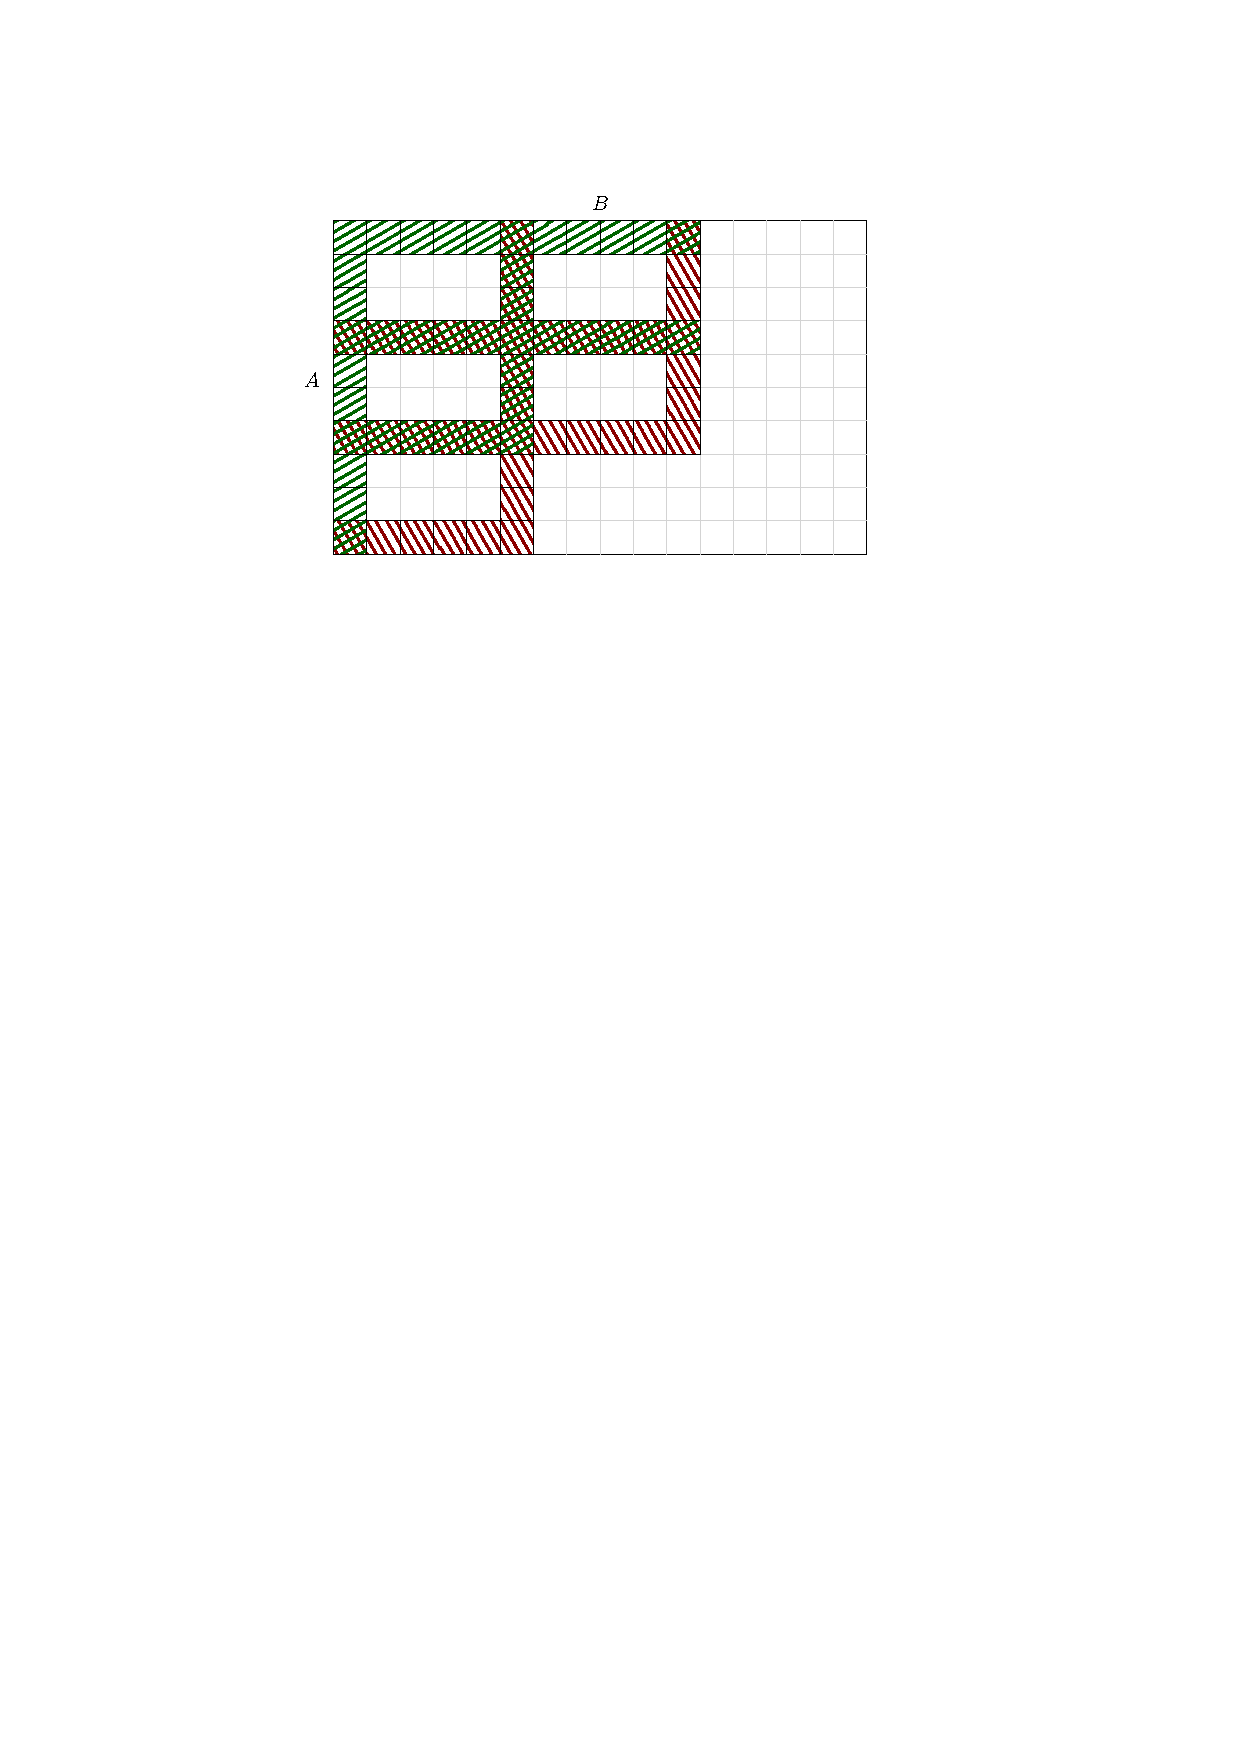
\includegraphics[width=7cm]{images/grid-dist-2}
  \caption{Shows hows blocks of the dynamic programming table fits together. Illustrates that no work needs to be done for the entries inside each block.}
  \label{fig:intro:dist-tables}
\end{figure}

Because consecutive values in the dynamic programming matrix can change by at most $1$, the representation can be succinctly represented and efficiently looked up. The pre-computed tables are then used to fill out the original dynamic programming matrix block-by-block.

It was found by \cite{LasseFourRussian} that the Four Russian approach improves the running time of the simple algorithm by a factor of around $6$ to $8$. This is worth keeping in mind when comparing the performance of the compression based algorithm examined in this thesis to the simple algorithm.

\subsection{Run-Length Encoding approach}
As mentioned in the introduction, the algorithm of \cite{Gawrychowski:2012:FAC:2422024.2422048} implemented and benchmarked in this thesis has a theoretical running time of $O(n N \sqrt{\log{\frac{N}{n}}})$. That is, it depends on the original length of the input and not only the length of the compressed strings.

There exist other approaches where the running time depends only on the lengths of the compressed strings. Such an algorithm was given by \cite{Chen:2010:FCA:1888935.1888984} which is based on run-length encoding. The run-length encoding of a string consists of a sequences of runs. A run consist of a count and a symbol and represents the symbol occurring count times. For example, the run-length encoding $\text{\texttt{a}}^4\text{\texttt{c}}^3\text{\texttt{g}}^1\text{\texttt{a}}^2\text{\texttt{t}}^2$ represents the string \texttt{aaaacccgaatt}. Notice that the run-length encoding may use more space than the original string if the input string does not contain a lot of repeating symbols. 

Assume that the input strings compress into run-length encodings consisting of respectively $m$ and $n$ runs where $m \leq n$. The running time for computing the edit-distance presented in \cite{Chen:2010:FCA:1888935.1888984} is $O(mn^2)$.

The running time only depends on the compressed lengths of the strings, however it is easy to construct input strings, where the algorithm is a factor of the string length slower than the simple algorithm, by exploiting the simplicity of the run-length encoding scheme.

An important feature of the algorithm benchmarked in this thesis is that it will never have a theoretically worse running time than the simple algorithm.

\subsection{Straight-line program approach}
\label{sec:edit-dist-on-slps-steps}
This section gives a very brief overview of the algorithm given by \cite{Gawrychowski:2012:FAC:2422024.2422048}, which is the main focus of this thesis. A more detailed description of each of the steps of the algorithm will be given later in this report. 

The key to make the algorithm work, is to compress the input strings to what is known as straight-line programs (SLPs). A formal definition of a SLP will be given in \cref{ch:compressing-strings}. For now it is sufficient to note that a SLP is a restricted context-free grammar.

The algorithm can be seen as a generalization of the Four Russian approach, where the blocking of the dynamic programming table is based on the productions of the SLPs, so that reused productions result in reusable blocks when filling out the grid. The algorithm can be summarized in the following steps:
\begin{itemize}
  \item Construct SLP representations $\SLP{A}$, $\SLP{B}$ of the two input strings $\str{A}{0}{m}$ and $\str{B}{0}{n}$. The better the compression scheme is able to compress the SLP representations the faster the algorithm will be. A natural trade-off arises in this step, namely the running time of the compression scheme versus the quality of the resulting compression. This step will be discussed in \cref{ch:compressing-strings}.
  \item Productions from the SLPs generating strings of length $O(x)$ for some fixed $x$ are selected in such a way that they cover the entire string without duplication. This can be done in $O(N)$ time by traversing the productions of the SLP bottom-up as described in \cref{sec:algorithm:select-productions}.
  \item Blocks from the dynamic programming table are precomputed for all the selected productions (these precomputed tables are called DIST tables). By naively representing the DIST tables they take up $O(x^2)$ space each, but using a succinct representation given in \cite{DBLP:journals/corr/abs-0707-3619}, it is possibly to reduce the space consumption to $O(x)$ and also improve the time it takes to use a $\DIST$ table. This step is described in \cref{sec:algorithm:building-DISTs-overview}.
  \item The dynamical programming table is filled up by using the partition and the precomputed $\DIST$ tables. This step takes time $O\left(\left(\frac{N}{x}\right)^2 \cdot AP(x)\right)$ where $AP(x)$ is the time to apply a DIST table. Using the succinct representation, \cite{Gawrychowski:2012:FAC:2422024.2422048} shows how to make $AP(x) = O(x)$, leading to a total running time of $O(\frac{N^2}{x})$. This step is described in \cref{sec:algorithm:filling-grid-overview}.
\end{itemize}

\chapter{Compressing input strings to straight-line programs}
\label{ch:compressing-strings}
There exist a large number of compression schemes for compressing strings, spanning both lossy and lossless schemes. Since it is desired that the edit distance algorithm always gives the correct result, only lossless compression schemes are considered.

The algorithm examined in this thesis is working over straight-line programs (SLPs), whereby only compression to this encoding is considered.
\begin{mydef}
  \label{def:slp}
  A straight-line program (SLP) is a restricted context-free grammar $G = (V, T, R, S)$, where
  \begin{itemize}
    \item $V = \{ S_1, \dots, S_k\}$ is an ordered set of non-terminals
    \item $T = \{ S_{k + 1}, \dots, S_{k + l} \}$ is an ordered set of terminals
    \item $R$ is a set of production rules mapping $V$ to $(V \cup T)^2$, with the condition that if $(S_i \to S_jS_k) \in R$, then $j,k \geq i$. This ensures that a SLP generates exactly one string.
    \item The start production $S = S_1$.
  \end{itemize}
  The size of a SLP is defined to be $|V \cup T|$, which is only a constant from the actual space consumption of a simple pointer-based SLP implementation.
\end{mydef}
From this definition it is not possible for a SLP to generate the empty string, however this poses no problem in practice as that case can be handled separately. An example of a SLP is shown in \cref{fig:slp-example}.
\begin{figure}[!htb]
  \centering
  \includegraphics[width=8cm]{images/slp-example}
  \caption{An example of a SLP generating the string \texttt{AAAABBABAAAAB}. The SLP is generated using the algorithm described in \cref{sec:compression:alg}.}
  \label{fig:slp-example}
\end{figure}

\begin{problem}
  \label{compression:problem:minimum-slp}
  Given an input string $\str{A}{0}{m}$ find a SLP $\SLP{A}$ of minimum size generating $A$.
\end{problem}
It is known from \cite[p. 212]{Rytter2003211} that this problem is NP-complete, hence a general, exact and efficient algorithm should not be expected to be easily obtainable. However, a number of articles (ex. \cite{Rytter2003211} and \cite{Sakamoto2005416}) have studied how to approximate a minimum size SLP for the input string. The approach implemented in this thesis is a $O(\log{m})$-approximation given in \cite{Rytter2003211}. This compression algorithm is based on the Lempel-Ziv factorization (LZ-factorization), which is a version of the popular LZ77 compression scheme. The algorithm is described in \cref{sec:compression:alg}.

A small theoretical improvement was given in \cite{Rytter2003211}, reducing the approximation factor to $O(\log{\frac{m}{g^*}})$ where $g^*$ denotes the size of the minimal SLP compression. As suggested by \cite{Rytter2003211} the improvement is mostly cosmetic, and from the description of the approach, I find it very likely that the approach will increase the constant in front of the big-$O$ notation. Therefore, I have not chosen to implement this theoretical improvement.

For computing the LZ-factorization a suffix tree is used. Suffix trees often come with a large constant space overhead, in some cases making them undesirable in practice. \cite{Sakamoto2005416} gave another algorithm for solving \cref{compression:problem:minimum-slp} which also achieves the $O(\log{\frac{m}{g^*}})$ approximation factor, but does so based on the RE-PAIR encoding scheme, which can be made to work without using a suffix tree. The reason for not implementing this approach, is that I find the LZ-factorization approach more intuitive, and for the benchmarks in this report the space consumption of the suffix tree has not been a problem.

In other areas of lossless compression, ex. bzip2 compression, the input string is encoded using a Burrows-Wheeler transform (BWT) \cite{BurrowsWheeler}. The intuition why the BWT works, is that it permutes the string in such a way that highly repetitive parts of the string are grouped together, making them easier to compress. However building the SLP over the BWT of the input string will not work because the BTW permutes the string, such that productions of the SLP does not corresponds to a continuous area in the input string. I have not been able to find any articles able to take advantage of the BWT for SLP based compression.

In lossless compression there exist Entropy-based encoding schemes. Such schemes uses the frequencies of the appearing alphabet symbols in the string to compress them to use as few bits as possible. This type of compression is not of significant interest in this context, since it is only of interest to minimize the number of productions in the resulting SLP.

\paragraph{Notes about size}
Given input strings over the finite alphabet $\Gamma$, all strings over this alphabet can trivially be encoded using $\ceil{\log_2 |\Gamma|}$ bits per symbol. However, for a direct representation of the SLP using pointers, a left and a right pointer has to be stored together with the symbol, which on a new machine uses up $64$ bits each. Moreover, the algorithms working on the SLPs are likely to require more information annotated to each node in the tree. This results in a huge constant blow up on the space required to store the input string, especially for strings not compressing very well.

It could be both of practical and theoretical interest to find a succinct representation of a SLP, in order to make the space consumption smaller. This would potentially make the SLP approach practical for long strings that does not compress very well.

\section{Algorithm}
\label{sec:compression:alg}
The idea behind the algorithm is to iteratively build the SLP for the string. This incremental building process will be based on repeating parts of the string called the LZ-factorization, which will be described after the overview of the algorithm has been given. The overall algorithm is given in \cref{alg:compression:approx}.
\enlargethispage{\baselineskip}

\begin{algorithm}[H]
  \label{alg:compression:approx}
  Let $\SLP{A}$ be an empty SLP\;
  Construct LZ-Factorization $f_1,\dots,f_k$ of the input string $\str{A}{0}{m}$\;
  \For{$i = 1, \dots, k$}{
    Find productions $S_1,\dots,S_{k_i}$ in the current SLP $\SLP{A}$ generating $f_i$\;
    Set $\SLP{S} = Concat(S_1,\dots,S_{k_i})$\;
    $\SLP{A} = Concat(\SLP{A}, \SLP{S})$\;
  }
  \Return $\SLP{A}$
  \caption{Algorithm for generating a $O(\log{m})$ approximation of the minimal SLP of the input string $\str{A}{0}{m}$.}
\end{algorithm}

The invariant of the algorithm is the following: After every iteration of the for-loop, it is the case that $\SLP{A}$ generates $\substr{A}{0}{|f_1| + \dots + |f_i|}$.

When building the SLP it will be considered as an AVL-tree. Therefore it is known how to search and concatenate two SLPs in a way that keeps the resulting SLP balanced. As mentioned, the idea is to add a repeating factor in the string one at a time. The repeating factor is added by reusing the productions already in the SLP generating the factor. During the concatenating operation, the resulting tree is balanced using appropriate AVL-tree rotations.

The $Concat$ process referenced in the code, is function almost the same way as concatenating two AVL trees. The only difference is that productions in the SLP may be shared, hence when adding nodes and making rotations, special care needs to be taken in order to ensure the balance of the tree and that the derived string is correct. This is easy to fix simply by introducing a constant number of new productions for every insertion and rotation. It is shown in \cite[p. 215, Lemma 2]{Rytter2003211} that this does not add too many in order to satisfy the $O(\log{m})$ approximation factor.

\paragraph{LZ-Factorization}
The factors iteratively added to the SLP are the LZ-factors of the input string $f_1 f_2 \dots f_k = \str{A}{0}{m}$, where $f_1 = A[0]$ and for $i \in \{2 \dots k\}$ $f_i$ is the longest prefix of $f_i \dots f_k$ occurring in $f_1 \dots f_{i - 1}$.

The LZ-factors of a string can be found by scanning the string from left to right. Assume that the current position is $i \in \{0, \dots, m - 1\}$, then the next LZ factor is found by finding the longest string starting at position $i$ that have occurred in the input string before position $i$. \Cref{fig:lz-factor} illustrates the situation.

\begin{figure}[!htb]
  \centering
  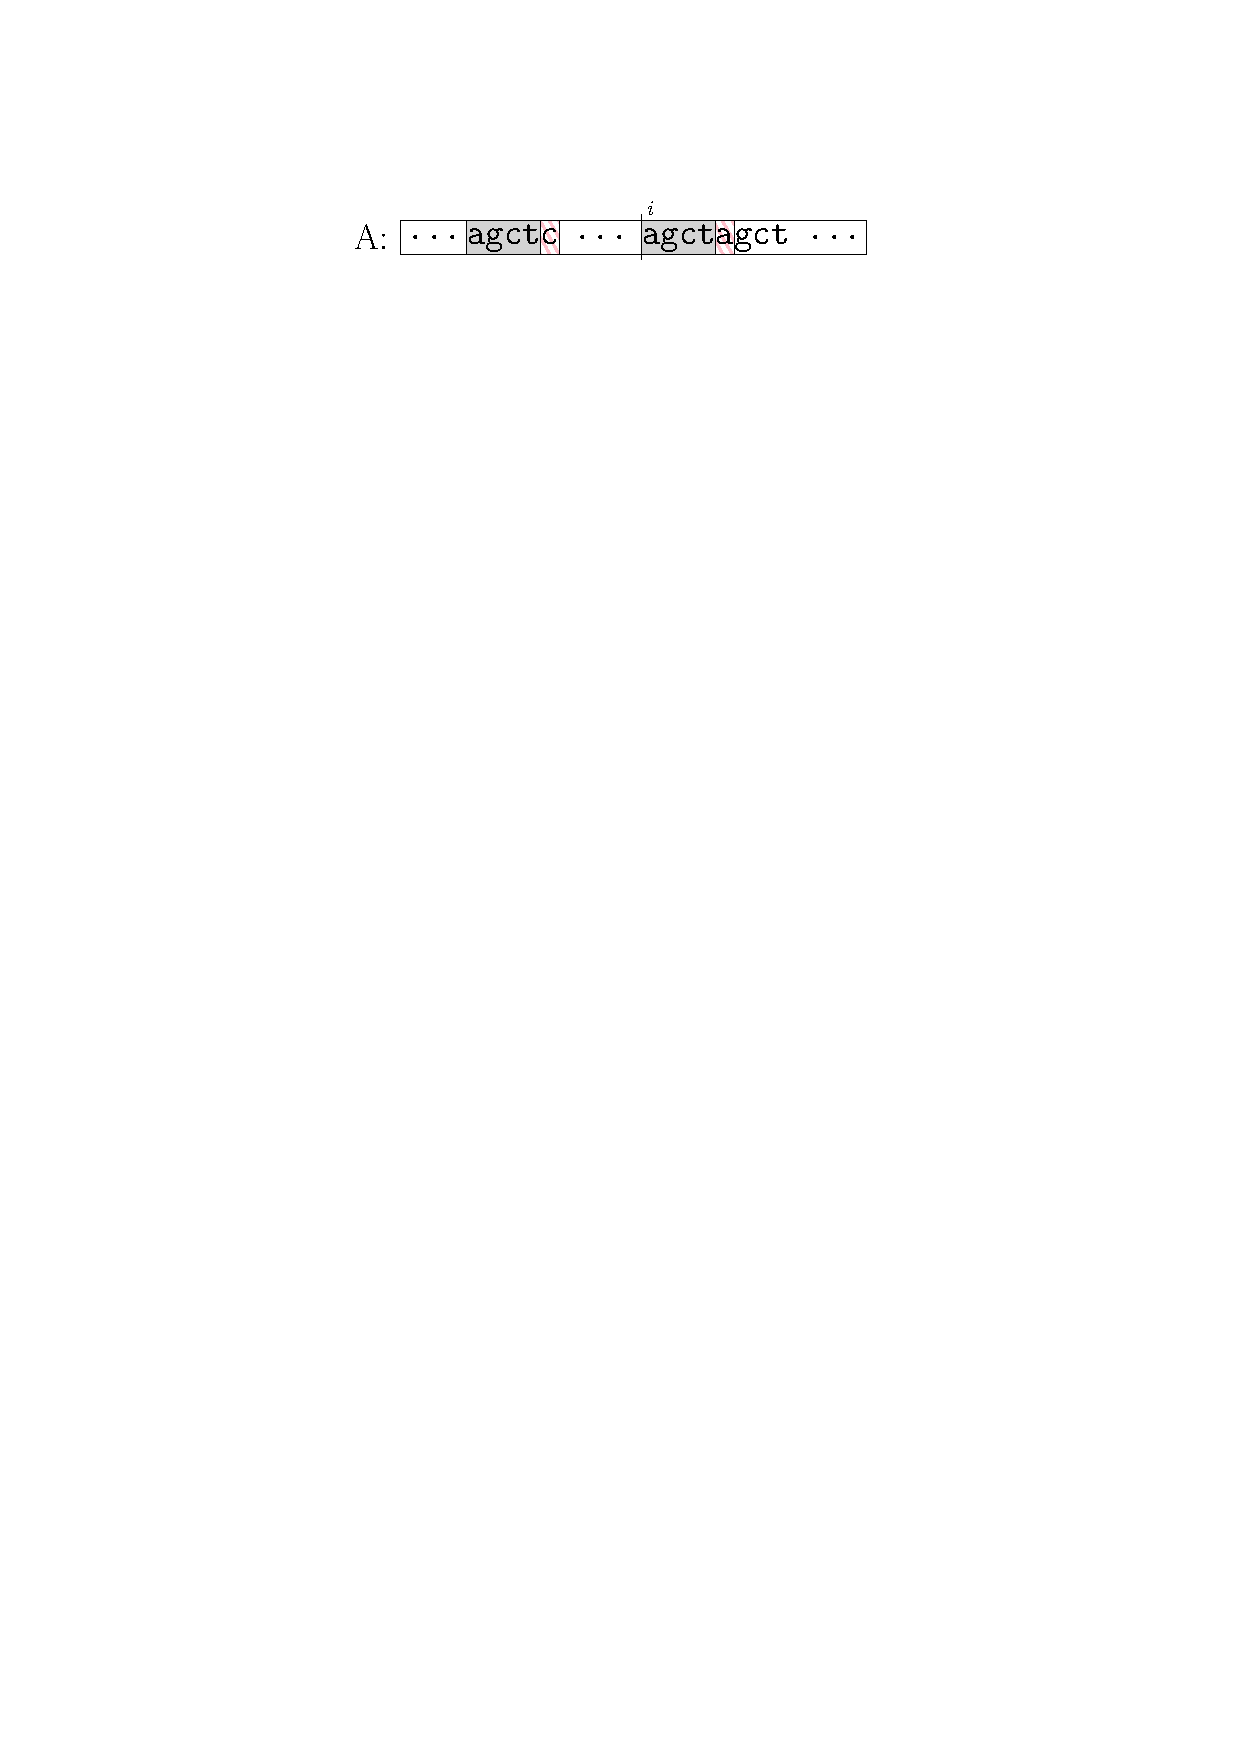
\includegraphics[width=10cm]{images/lz-factor}
  \caption{A graphical illustration of a LZ-factor.}
  \label{fig:lz-factor}
\end{figure}

It is required to be able to efficiently find the nodes in the current SLP which generates a LZ factor. In order to do this, the LZ factors of the string are specified by their first occurrence in the input string by indices. That is, $f_i$ is identified by two indices $p, q$ such that $f_i = \substr{A}{p}{q}$ where $p,q \in \mathbb{N}$ and $p < q \leq |f_1 \dots f_{i - 1}|$.

Using these indices it is easy to find the corresponding productions in the SLP by annotating the derived length for each of the productions, and then make a top-down descent of the tree checking if the interval overlaps the current node.

\paragraph{Computing the LZ-factorization}
The only step of the SLP construction algorithm not thoroughly described in \cite{Rytter2003211}, is how to compute the LZ-factorization of a string efficiently. They only state that it can be done efficiently using a suffix tree. Although the algorithm is quite simple, it is included in this report for completeness.

First the suffix tree for the input string is built. Then every node $v$ in the suffix tree is annotated with the first index in the string where the substring spelled out from the root to $v$ occurs. This is done by traversing the tree bottom up. Any leaf is annotated by its suffix number and any non-leaf is annotated by the minimum over its children.

Having the described suffix tree, the LZ-factorization can be found by scanning the input string and follow the corresponding path in the suffix tree. While the string spelled out from the root to the current node has already occurred before in the string, the path is extended. Otherwise a new LZ factor is added and the search begins from the top of the suffix tree. Pseudo code for the algorithm is given in \cref{alg:compression:lz-factorization}. The algorithm could potentially be improved a bit by following an entire suffix tree edge in every iteration. However, since the SLP construction is not the time consuming part of the algorithm this has not been implemented as the gain will be almost non noticeable.

The total time for computing the LZ factorization of a string of length $m$ is bounded by $O(m\log{\Gamma})$, where there $\log{\Gamma}$ factor comes from the used suffix tree \cite{SDSL}. Because the alphabet in this thesis is assumed to be of constant size, the LZ factorization can be computed in linear time.

\begin{center}
  \begin{algorithm}[!htb]
    \label{alg:compression:lz-factorization}
    $LZFactors = \emptyset$\;
    $factorStart = 0$\;
    \While{$factorStart < |A|$}{
      $previousNode = currentNode = Root$\;
      $currentEdgeLength = currentEdgeMatched = 0$\;

      $factorLen = 1$\;
      \While{true}{
        \If{$currentEdgeMatched \geq currentEdgeLength$}{
          $previousNode = currentNode$\;
          $pos = factorStart + factorLen - 1$\;
          $currentNode, followedEdge = \operatorname{FastScan}(currentNode, A[pos])$\;
          $currentEdgeLength = |followedEdge|$\;
          $currentEdgeMatched = 0$\;
        }

        \If{$FirstSeen[Root \to currentNode] + factorLen - 1 \geq factorStart$}{
          \eIf{$factorLen == 1$}{
            $LZFactors = LZFactors \cup \{ (factorStart, factorStart) \}$\;
            $factorStart = factorStart + 1$\;
          }{
            $pos = FirstSeen[Root \to previousNode]$\;
            $LZFactors = LZFators \cup \{ (pos, pos + factorLen - 2) \}$\;
            $factorStart = factorStart + factorLen - 1$\;
          }

          break\;
        }

        $previousNode = currentNode$\;
        $currentEdgeMatched = currentEdgeMatched + 1$\;
        $factorLen = factorLen + 1$\;
      }
    }
    \Return $LZFactors$
    \caption{Algorithm for generating the LZ-factorization of a given input string $A$. The algorithm assumes a $FirstSeen$ array that for a given node gives the first time its associated string occurs in the string.}
  \end{algorithm}
\end{center}

\paragraph{Implementation details}
The implementation uses a pointer based representation of the SLP. It is worth noticing that in the context of standard binary heaps, pointer based implementation typically performs worse than an implicit array representation due to the extra overhead of lookup pointers and jumping in memory. In a previous project \cite[p. 9]{AA13Project1} the penalty of using pointers was found to be around a running time factor of $2$.

It is also expected that a pointer based SLP will suffer for such a penalty when traversing the tree. However, since the SLP does not have a fixed topology, the pointer based solution is the easiest way to represent the topology. It may be the case that this could be encoded in some clever way in combination with a succinct representation of a SLP, but this is outside the scope of this thesis.

\clearpage
\section{Benchmarks}
\label{sec:compression:benchmarks}
This section will examine how well different types of strings can be compressed to SLPs. It will also be verified that the theoretical running time of $O(m\log{m})$ is satisfied in practice for a input string $\str{A}{0}{m}$.

\subsection{Compression quality}
First the quality of the compressions is examined for the different types of input as described in \cref{sec:intro:test-data}.

\subsubsection{Fibonacci strings}
\label{sec:compressing-Fibonacci-strings}
When evaluating the quality of compressed Fibonacci strings, it is useful to consider how well they can be compressed to a SLP. For this reason recall the definition of Fibonacci strings:
\begin{align*}
  F_1 &= \text{a} \\
  F_2 &= \text{ab} \\
  F_{i} &= F_{i - 1} F_{i - 2} \quad\quad \text{for } i \geq 3
\end{align*}
Notice directly by definition, $F_1$ can be represented by a SLP of size $1$ and $F_2$ can be represented by a SLP of size $3$. Constructing $F_{i + 1}$ for $i > 2$ can be done by adding one extra production to the SLP describing $F_{i}$.

Therefore Fibonacci strings compress very well to a SLP, where a representation of $F_{i}$ uses only $i + 1$ productions for $i \geq 2$. It is noticed in \cref{claim:fib-slp-optimal} that there is no smaller grammar generating Fibonacci strings.

\begin{claim}
  \label{claim:fib-slp-optimal}
  The described SLPs for the Fibonacci strings are optimal.
  \begin{proof}
    From the definition of Fibonacci strings it can be seen that the $i$'th Fibonacci string, $F_i$, has $i$ LZ-Factors. This follows since the $F_{i-2}$ factor in $F_i = F_{i - 1} F_{i - 2}$ will always occur before in the strings and therefore will contribute exactly one LZ-factor.

    By a slight modification of \cite[Theorem 1]{Rytter2003211} where it is used that a SLP for a Fibonacci strings must have at least two non-terminals, it is found that for all grammars $G_i$ deriving $F_i$ it must be the case that $i + 1 = |LZ(F_i)| + 1 \leq |G_i|$. Therefore it must be the case that the previously described grammars for the Fibonacci strings are optimal.
  \end{proof}
\end{claim}

Using this, the quality of the compressed Fibonacci strings can be measured relative to the optimal SLP. \Cref{fig:compression:quality:fibonacci} shows a plot where the blue line shows how big a factor the computed SLP is bigger than the optimal SLP.

By the proof in \cite{Rytter2003211} this overhead should be bounded by $O(\log{m})$. The green line of \cref{fig:compression:quality:fibonacci} plots the production overhead normalized by $\log{m}$. From theory this should converge towards a constant, which also seems to be the case in practice.

As mentioned above, it is easy to construct a SLP of size $n = O(\log{m})$ for a Fibonacci string of length $m$. Because of the approximation factor in the SLP approximation algorithm, this bound worsens to $O(\log^2{m})$. From \cref{fig:compression:quality:fibonacci} it is seems that the $O(\log{m})$ bound is not satisfied but that the $O(\log^2{m})$ bound is.

All following benchmarks in the report are using the SLP constructed by the approximation algorithm. That is, for all benchmarks the Fibonacci strings compress such that $n = O(\log^2{m})$.
%
\begin{figure}[h!]
  \centering
  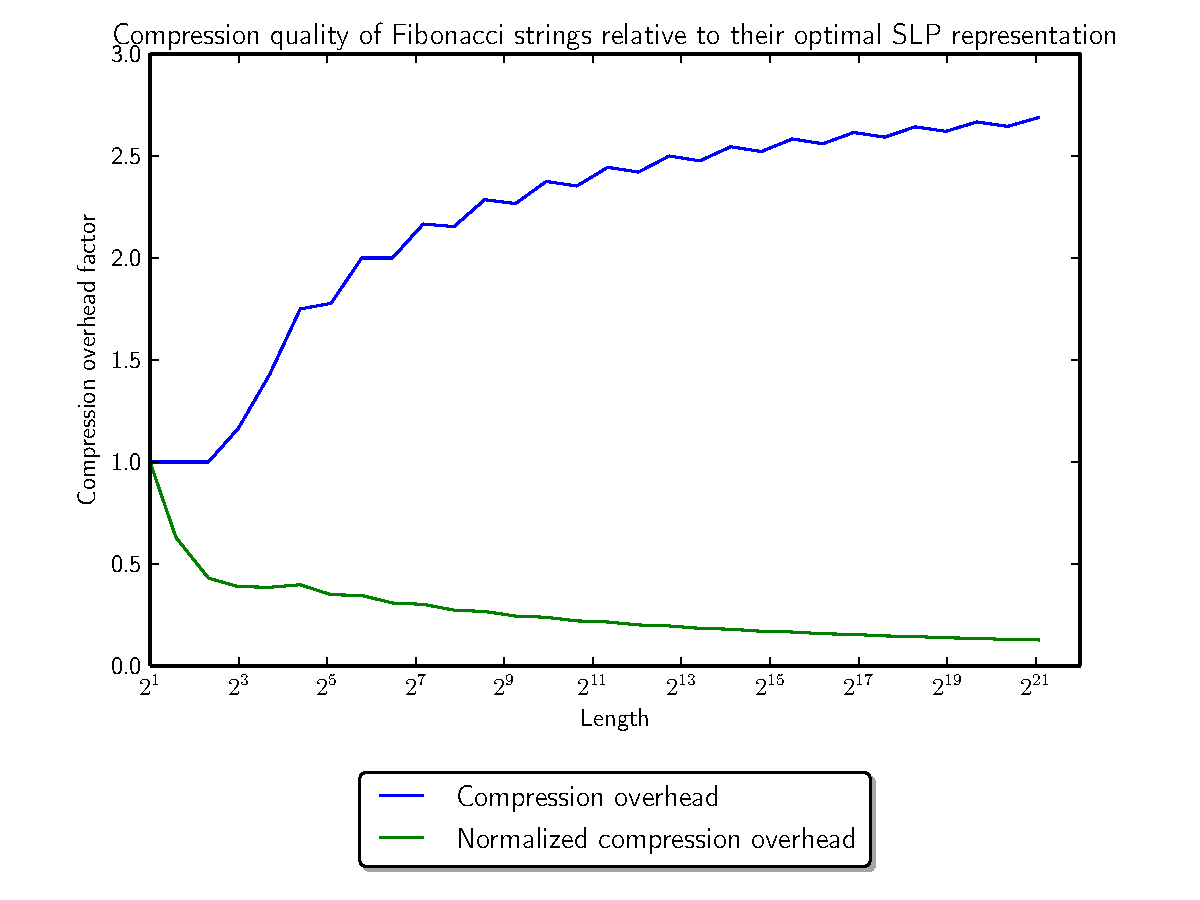
\includegraphics[width=11cm]{compression/fib}
  \caption{Plot of how well Fibonacci strings compress to a SLP relative to the minimal SLP describing the corresponding Fibonacci string.}
  \label{fig:compression:quality:fibonacci}
\end{figure}

\subsubsection{Random strings}
In these benchmarks the compressibility in terms of the compression ratio to the original input is examined. A new random string has been generated for every benchmarked input length.

Random strings should contain no systematic patterns and will by design maximize the average information rate, which by information theory should make them very hard to compress. The only type of compression in this type of string is expected to occur because the alphabet is of constant size and the strings are of arbitrary length.

It can be seen on \cref{fig:compression:quality:random} that the compression ratio of the string is decreasing as the input size gets larger. For the largest input sizes, \cref{fig:compression:quality:random} shows that the corresponding SLP is approximately half the size of original input length. This behavior is expected due to the constant alphabet size, which is also why the Four Russian approach sketched in \cref{sec:4-russian} works.
%
\begin{figure}[h!]
  \centering
  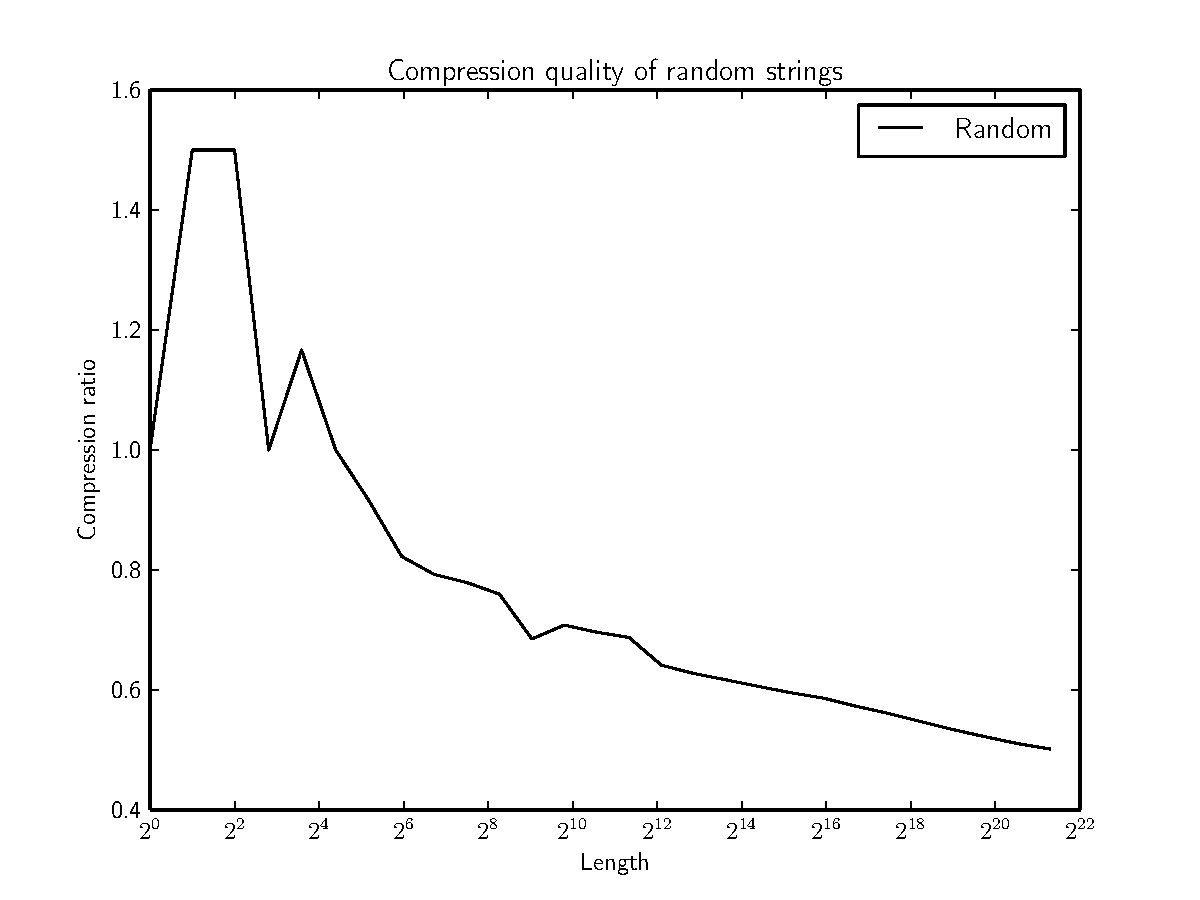
\includegraphics[width=11cm]{compression/random}
  \caption{Plot of compression quality for random strings.}
  \label{fig:compression:quality:random}
\end{figure}

\subsubsection{Human Genome}
Like for the random strings, the compressibility of the human genome is examined by considering how the compression ratio is behaving. Since there only is one human genome of a specific length, it is not possible to directly vary the input size as for the random strings. Instead it has been chosen to use prefix of the human genome sequences. This choice may be a bit misleading for small prefix lengths since the distribution of nucleotides may be different in the beginning of the string than in other parts. However, as the selected prefixes gets longer this should even out, and the actual compressibility of the string should be accurately measured.

\Cref{fig:compression:quality:hg} shows a plot of the compression ratios for the human genome data sets. It can be seen that the non-repetitive part of the human genome is close to the compression ratio of a random string. It drops somewhat below the compression ratio for random string around $m = 2^{18}$, however as the string size grows, it seems to converge to the compression ratio for the random string again.

The compression ratios for the combined and repetitive test cases are exactly the same until around $m = 2^{10}$. This is because the first part of the combined human genome is a repetitive region, hence the first prefixes of these strings are the same. In the beginning the repetitive string compresses significantly better than the random string, but as the prefix length grows the compression ratio is only a bit below the compression ratio for random strings.

Since random strings should not compress very well, it is not desirable that the human genome, which is considered to be a realistic type of input, only compresses a little better. However, the compression factor is still $\approx 0.4$ for large input, and therefore there is still hope that the edit distance algorithm based on SLP compression may perform better than the simple edit distance algorithm.

\begin{figure}[h!]
  \centering
  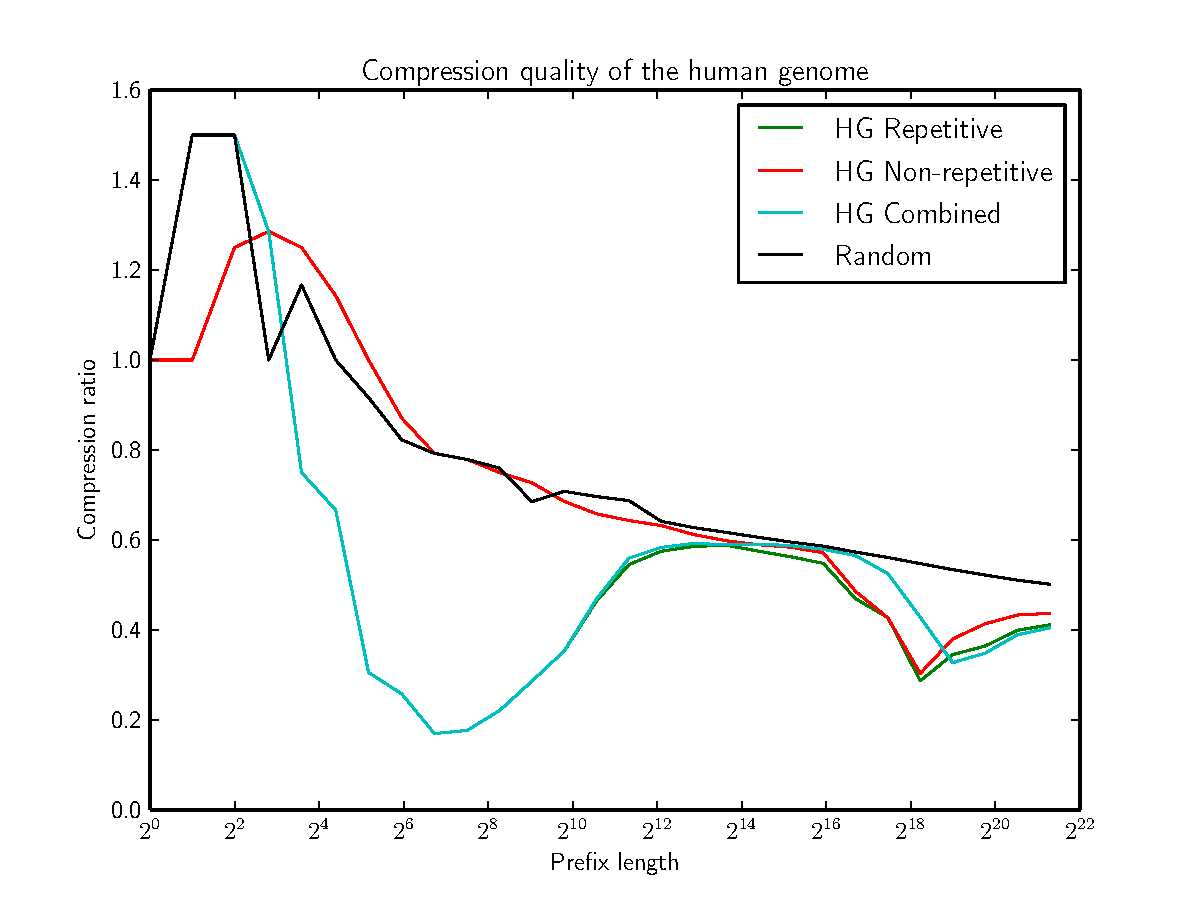
\includegraphics[width=11cm]{compression/hg}
  \caption{Plot of how well the human genome of \cref{sec:intro:test-data} compresses compared to a random string.}
  \label{fig:compression:quality:hg}
\end{figure}

\subsection{Running time}
The running time of the algorithm is bounded by $O(m\log{m})$ for a input string $\str{A}{0}{m}$. This follows since the LZ-factorization $f_1, \dots, f_k$ can be found in linear time and the concatenation and search steps all can be done in time $O(\log{m} + \log{|f_i|}) = O(\log{m})$ for each factor $f_i$. Because $k = O(m)$ the running time follows.

\Cref{fig:compression:runningtime} shows the normalized running time for SLP construction. From the plot it can be seen that the normalized running time for the different types of input more or less converges to a constant. However, for the longest input sizes especially the human genome test cases seem to increase. \Cref{fig:compression:instructions} shows that the normalized instruction count does not have this increase, but that the L2 cache misses increases. Therefore the extra increase can be explained by the hierarchical memory layout of a modern computer.

An interesting thing to notice that is not explained by the theoretical running time bound, is that the normalized running times are stabilizing at different constants across the different input types. Before concluding that the theoretical running time seems to be satisfied up to the hierarchical memory layout, it is needed to argue that there does not exist types of input that result in arbitrarily large constants.

From the algorithm, the places where the running time may significantly differ for different types of input are when building the suffix tree and balancing the SLP. This matches well with \cref{fig:compression:runningtime} that suggests that input with a less repeating structure has a higher constant. When less of the input repeats more insertions are made into the SLP and more balancing is needed, which leads to a larger constant.

Because it is known that there can not exist input that performs too many tree rotations in the AVL tree, it is concluded that the running time in the implementation does satisfy the theoretical running time.

Therefore the construction of the SLP should not be the bottleneck of the combined edit distance algorithm, since it is asymptotically dominated by the other part of the algorithm doing the actual edit distance computation.
%
\begin{figure}[!htb]
  \centering
  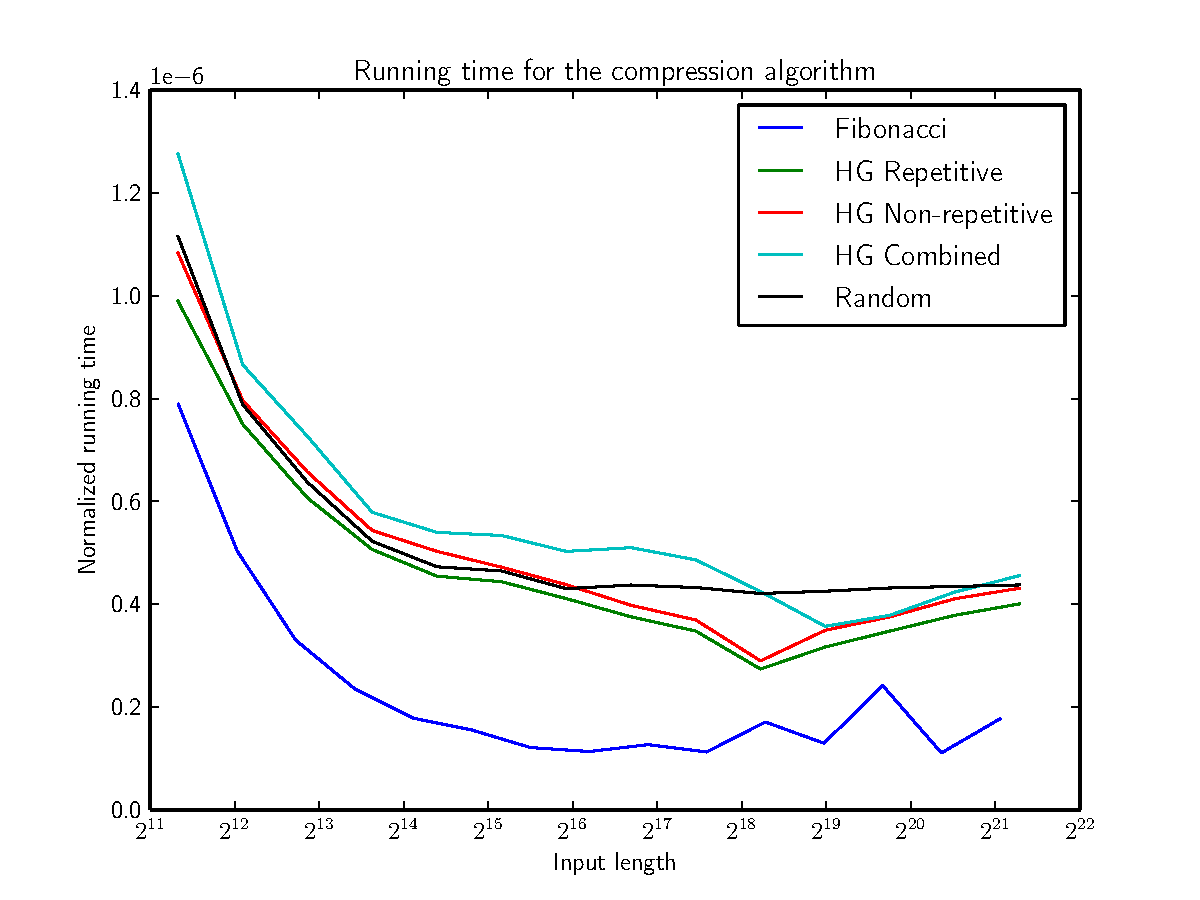
\includegraphics[width=11cm]{compression/runningtime}
  \caption{Normalized running time for construction of compressed SLP.}
  \label{fig:compression:runningtime}
\end{figure}

\begin{figure}[!htb]
  \centering
  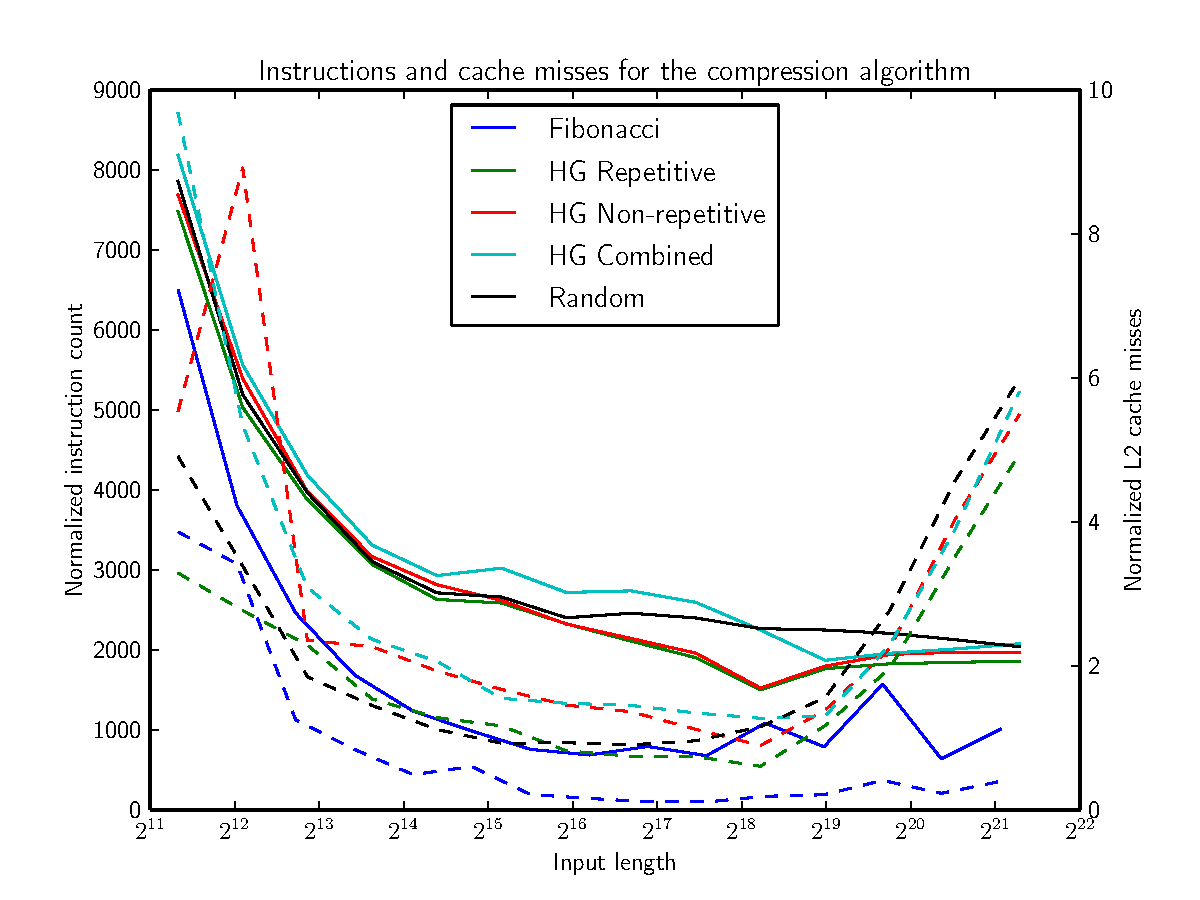
\includegraphics[width=11cm]{compression/instructions}
  \caption{Normalized instruction counts and L2 cache misses for construction of SLP. Solid lines are instructions, dashed lines are L2 cache misses.}
  \label{fig:compression:instructions}
\end{figure}

\chapter{SLP based edit distance algorithm}
\label{ch:algorithm}

This chapter will describe and benchmark the algorithm for computing the edit distance of two input SLPs $\SLP{A}$ and $\SLP{B}$.

\section{Preliminaries}
\label{sec:algorithm:preliminaries}
In order to describe the algorithm and argue its correctness, some notation will be introduced.

It has been chosen that all matrices used in this report are $0$-indexed. That is, an entry in a matrix $A$ of size $m \times n$ is indexed by $A(i, j)$ where $i \in \{0, \dots, m - 1\}, j \in \{0, \dots, n - 1\}$. Note that this is a different choice than the referenced literature describing the algorithm (most notably \cite{Tiskin:2010:FDM:1873601.1873704} and \cite{DBLP:journals/corr/abs-0707-3619}), who for convenience use odd half-integers to index some of the matrices. This approach was not chosen in order to make the calculations in this report closer to the actual \texttt{C++} implementation.

All matrices considered in this report will be square matrices, ie. of size $n \times n$ for some $n \in \mathbb{N}$. Therefore all following definitions will only be given for square matrices, but most of them could easily be generalized to matrices of arbitrary dimension.

\begin{mydef}
  A permutation matrix of size $n$ is a matrix over $\{0,1\}^{n \times n}$ where each row and each column contains exactly one $1$. That is, it can be seen as the identity matrix of size $n \times n$ where the rows (or columns) are permuted.
  It is assumed that the index of the column (row) containing the $1$ can be found in constant time from a given row (column).
\end{mydef}
The latter constraint on the query time of the $1$ entry is required to achieve the running time of some of the algorithms (ex \cref{lemma:simple-unit-monge-query-next}). The way permutation matrices are represented in the implementation, is that the row and column permutation are specified using $2n = O(n)$ machine words. This directly gives the constant time query to the $1$ entry of a given row/column.

The algorithm stores a lot of permutation matrices in memory. Therefore it is desirable to minimize the space consumption of these matrices. However, it turns out that the space consumption of $O(n)$ machine words is asymptotically optimal: A permutation matrix of size $n$ can express $n!$ different permutation matrices (since there are $n!$ different permutations of the rows of the identity matrix), hence at least $\Omega(\log{n!})$ bits are needed to represent a permutation matrix. By Stirling's approximation it is known that
\[
  \ln{n!} = n \ln{n} - n + O(\ln{n}),
\]
hence $\Omega(\log{n!}) = \Omega(n \log{n})$ bits are required to represent the permutation matrix, which is also what is used in the row/column-permutation representation.

\paragraph{Permutation matrix properties}
This section will define and classify different useful properties about matrices, where especially permutation matrices are of interest. 
%
\begin{mydef}
  The distribution matrix $A^{\Sigma}$ of a $n \times n$ matrix $A$ is a $(n + 1) \times (n + 1)$ matrix defined as
  \[
    A^{\Sigma}(i, j) = \sum_{\substack{\hat{i} \in \{i, \dots, n - 1\} \\ \hat{j} \in \{0, \dots, j - 1\}}} {A(\hat{i}, \hat{j})},
  \]
  or informally the sum of all entries in the sub-matrix to the left and below of a given entry $(i, j)$.
\end{mydef}
%
\begin{mydef}
  The density matrix $A^{\Box}$ of a $(n + 1) \times (n + 1)$ matrix is a $n \times n$ matrix defined as
  \[
    A^{\Box}(i, j) = A(i, j + 1) - A(i, j) - A(i + 1, j + 1) + A(i + 1, j)
  \]
  for all $i, j \in \{ 0, \dots, n - 1 \}$.
\end{mydef}%
The distribution and density operators always have the useful relation stated by the following claim.
\begin{claim}[\reftiskin{p. 1288}{mentioned but not proved}]
  \label{claim:sigma-box-identity}
  For any matrix $A$ of size $n \times n$ it is the case that
  \[
    (A^{\Sigma})^{\Box}(i, j) = A(i, j)
  \]
  \begin{proof}
    The proof follows directly by unfolding definitions:\\
    \scalebox{0.9}{\parbox{.5\linewidth}{%
    \begin{align*}
      (A^{\Sigma})^\Box(i, j) &= A^{\Sigma}(i, j + 1) - A^{\Sigma}(i, j) - A^{\Sigma}(i + 1, j + 1) + A^{\Sigma}(i + 1, j) \\
        &= \sum_{\substack{\hat{i} \in \{i, \dots, n - 1\} \\ \hat{j} \in \{0, \dots, j\}}} {A(\hat{i}, \hat{j})}
         - \sum_{\substack{\hat{i} \in \{i, \dots, n - 1\} \\ \hat{j} \in \{0, \dots, j - 1\}}} {A(\hat{i}, \hat{j})}
         - \sum_{\substack{\hat{i} \in \{i + 1, \dots, n - 1\} \\ \hat{j} \in \{0, \dots, j\}}} {A(\hat{i}, \hat{j})}
         + \sum_{\substack{\hat{i} \in \{i + 1, \dots, n - 1\} \\ \hat{j} \in \{0, \dots, j - 1\}}} {A(\hat{i}, \hat{j})} \\
        &= A(i, j)
    \end{align*}
    }}\\
  \end{proof}
\end{claim}
If the operators are applied in the opposite order, it will not always describe a identity transformation. A class of matrices with this property is defined.
\begin{mydef}[\reftiskin{p. 1288}{Definition 2.1}]
  \label{def:simple}
  A matrix $A$ is called simple if $(A^{\Box})^\Sigma = A$.
\end{mydef}
The set of simple matrices can be classified by the following claim.
\begin{claim}[\reftiskin{p. 1288}{remark without proof}]
  \label{claim:simple-matrix-characterization}
  A matrix $A$ of size $(n + 1) \times (n + 1)$ is simple iff $\forall i,j: A(n, j) = A(i, 0) = 0$, ie. iff the leftmost column and bottom row have all zero entries.
  \begin{proof}
    The proof follows almost directly by unfolding definitions. For all $i, j \in \{ 0, \dots, n \}$ it follows that%
    \begin{align*}
      (A^{\Box})^{\Sigma}(i, j) &= \left( \left\{ A(\hat{i}, \hat{j} + 1) - A(\hat{i}, \hat{j}) - A(\hat{i} + 1, \hat{j} + 1) + A(\hat{i} + 1, \hat{j}) \right\}_{\hat{i}, \hat{j}} \right)^{\Sigma}(i, j) \\
        &= \sum_{\substack{\hat{i} \in \{i, \dots, n - 1\} \\ \hat{j} \in \{0, \dots, j - 1\}}} { A(\hat{i}, \hat{j} + 1) - A(\hat{i}, \hat{j}) - A(\hat{i} + 1, \hat{j} + 1) + A(\hat{i} + 1, \hat{j}) } .
    \end{align*}%
    By splitting the sum on every term, changing indexes in the sum and using the definition of the $\Sigma$-operator, it is found that
    \begin{align*}
      (A^{\Box})^{\Sigma}(i, j) &=
        \begin{aligned}
          &A^{\Sigma}(i, j + 1) - \sum_{\mathclap{\hat{j} \in \{0, \dots, j\}}} A(n, \hat{j}) - \sum_{\mathclap{\hat{i} \in \{i, \dots, n\}}} {A(\hat{i}, 0)} \\
          - &\left( A^{\Sigma}(i, j) - \sum_{\mathclap{\hat{j} \in \{0, \dots, j - 1\}}} A(n, \hat{j}) \right) \\
          - &\left( A^{\Sigma}(i + 1, j + 1) - \sum_{\mathclap{\hat{i} \in \{i + 1, \dots, n\}}} A(\hat{i}, 0) \right) \\
          + &A^{\Sigma}(i + 1, j)
        \end{aligned} \\
        &= \sum_{\hat{i} \in \{i, \dots, n\}} A(\hat{i}, j) - \sum_{\hat{i} \in \{i + 1, \dots, n\}} A(\hat{i}, j) - A(n, j) - A(i, 0) \\
        &= A(i, j) - A(n, j) - A(i, 0).
    \end{align*}
    Therefore a matrix is simple iff $\forall i, j: A(i, 0) = -A(n, j)$ iff $\forall i, j: A(i, 0) = A(n, j) = 0$.
  \end{proof}
\end{claim}
%
\begin{mydef}[\reftiskin{p. 1288}{Definition 2.4}]
  A matrix $A$ is called Monge if $A^{\Box}$ is non-negative.
\end{mydef}
\begin{mydef}[\reftiskin{p. 1288}{Definition 2.6}]
  \label{def:unit-monge}
  A square matrix $A$ is called unit-Monge if $A^{\Box}$ is a permutation matrix.
\end{mydef}
It follows clearly that any unit-Monge matrix is also Monge since the identity matrix has no negative entries. The following lemma characterizes the unit-Monge matrices.
\begin{lemma}[\refbook{p. 10}{Lemma 2.11}]
  \label{lemma:unit-monge-characterization}
  Let $A \in \mathbb{N}^{(n + 1) \times (n + 1)}$ be a simple Monge matrix. Then $A$ is unit-Monge iff
  \[
    A(i, n) - A(i + 1, n) = 1 \quad \text{ and } \quad A(0, j + 1) - A(0, j) = 1
  \]
  for all $i, j \in \{0, \dots, n - 1\}$.
  \begin{proof}
    Since all entries of $A$ are natural numbers, the entries of $A^{\Box}$ are all integers directly by definition. Also, since $A$ is Monge, it is known that $A^{\Box}(i, j) \geq 0$ for all $i, j \in \{0, \dots, n - 1\}$. Therefore it can be noticed that $A^{\Box}$ is a permutation matrix iff
    \[
      \sum_{\hat{j} \in \{0, \dots, n - 1\}} A^{\Box}(i, \hat{j}) = 1
      \quad \text{ and } \quad
      \sum_{\hat{i} \in \{0, \dots, n - 1\}} A^{\Box}(\hat{i}, j) = 1
    \]
    for all $i, j \in \{0, \dots, n - 1\}$. Both of the sums can be written out to find that for all $i, j \in \{0, \dots, n - 1\}$:
    \begin{align*}
      \sum_{\hat{j} \in \{0, \dots, n - 1\}} A^{\Box}(i, \hat{j})
        &= \sum_{\hat{j} \in \{0, \dots, n - 1\}} \left( A(i, \hat{j} + 1) - A(i, \hat{j}) - A(i + 1, \hat{j} + 1) + A(i + 1, \hat {j}) \right) \\
        &= A(i, n) - A(i, 0) - A(i + 1, n) + A(i + 1, 0) \\
        \text{\cref{claim:simple-matrix-characterization}} &= A(i, n) - A(i + 1, n)
    \end{align*}
    \begin{align*}
      \sum_{\hat{i} \in \{0, \dots, n - 1\}} A^{\Box}(\hat{i}, j)
        &= \sum_{\hat{i} \in \{0, \dots, n - 1\}} \left( A(\hat{i}, j + 1) - A(\hat{i}, j) - A(\hat{i} + 1, j + 1) + A(\hat{i} + 1, j) \right) \\
        &= A(0, j + 1) - A(n, j + 1) - A(0, j) + A(n, j) \\
        \text{\cref{claim:simple-matrix-characterization}} &= A(0, j + 1) - A(0, j)
    \end{align*}
    Therefore $A^{\Box}$ is a permutation matrix (i.e. $A$ is unit-Monge) iff
    \[
      A(i, n) - A(i + 1, n) = 1 \quad \text{ and } \quad A(0, j + 1) - A(0, j) = 1
    \]
    for all $i, j \in \{0, \dots, n - 1\}$.
  \end{proof}
\end{lemma}
Notice that if a matrix $A$ is both simple and unit-Monge (from now on denoted simple unit-Monge), then from the unit-Monge property, there exists some permutation matrix $P$ such that $P = A^{\Box}$, and by applying the $\Sigma$-operator and using the simple property, it is found that $P^\Sigma = (A^{\Box})^{\Sigma} = A$. Therefore a simple unit-Monge matrix can be represented in linear space by a permutation matrix.

An important observation required for the algorithm described in \cref{sec:algorithm:min-mult-two-unit-monge} is the following.
\begin{lemma}[\reftiskin{p. 1288}{Theorem 2.1}]
  \label{lemma:simple-unit-monge-query-next}
  Given a permutation matrix of size $n$, then given the value of $P^{\Sigma}(i, j)$ for some $i, j \in \{0, \dots, n\}$, the adjacent entries $P^{\Sigma}(i \pm 1, j), P^{\Sigma}(i, j \pm 1)$ where they exist, can be computed in constant time.
  \begin{proof}
    Because a permutation matrix $P$ only contains a single $1$ in any row or column, the value of adjacent entries in $P^{\Sigma}$ can only differ by either $-1$, $0$ or $1$. Determining which is the case is easy by looking at the query direction and in which column (row) the $1$ entry in $P$ is located.

    For example, to query the entry to the right of the given entry, it is easily seen that
    \begin{align*}
      P^{\Sigma}(i, j + 1) &= \sum_{\substack{\hat{i} \in \{i, \dots, n - 1\} \\ \hat{j} \in \{0, \dots, j\}}} P(\hat{i}, \hat{j})
        = \sum_{\substack{\hat{i} \in \{i, \dots, n - 1\} \\ \hat{j} \in \{0, \dots, j - 1\}}} P(\hat{i}, \hat{j}) + \sum_{\hat{i} \in \{i, \dots, n - 1\}} P(\hat{i}, j) \\
        &= P^{\Sigma}(i, j) + \begin{cases}
            1  & \text{if position of $1$ in $j$'th row of $P \geq i$} \\
            0  & \text{o/w}
          \end{cases},
    \end{align*}
    where the latter can be calculated in $O(1)$ time by the assumption of constant query time on permutation matrices.
  \end{proof}
\end{lemma}

\begin{mydef}[\reftiskin{p. 1289}{Definition 3.1}]
  \label{def:minimum-distance-product}
  Given two matrices $A, B$ both of size $n \times n$ their minimum distance product is a $n \times n$ matrix denoted by $A \odot B$ and is given by
  \[
    (A \odot B)(i, j) = \min_{k \in \{ 0, \dots, n - 1 \}} \left( A(i, k) + B(k, j) \right)
  \]
  for all $i, j \in \{0, \dots, n - 1\}$.
  The maximum distance product is defined analogously but where the $\min$ is replaced by $\max$.
\end{mydef}
The algorithm relies on the following claim, which implies the minimum distance product of two simple unit-Monge can be succinctly represented by a permutation matrix.
\begin{claim}[\refbook{p. 16}{Theorem 3.4}]
  \label{claim:unit-monge-min-prod-closed}
  Given two simple unit-Monge matrices $A, B$, then their minimum distance product $A \odot B$ is also simple unit-Monge.
\end{claim}
As the proof of \cref{claim:unit-monge-min-prod-closed} is thoroughly described in \cite[Theorem 3.4, p. 16]{DBLP:journals/corr/abs-0707-3619} and that the statement of \cref{claim:unit-monge-min-prod-closed} is not used directly in the theorems and lemmas establishing the correctness of the algorithm, the proof is not included in this thesis. \Cref{claim:unit-monge-min-prod-closed} is used to give rise to the following notation that turns out useful later.
\begin{mydef}[\reftiskin{p. 1289}{Definition 3.2}]
  Given permutation matrices $P_A$ and $P_B$, then $P_A \boxdot P_B = P_C$ if $P_C^{\Sigma} = P_A^{\Sigma} \odot P_B^{\Sigma}$.
\end{mydef}

\section{Algorithm}
The algorithm follows the steps in \cref{sec:edit-dist-on-slps-steps}, however instead of directly computing the edit distance between the two input SLPs, the longest common substring (LCS) between the two SLPs will be computed. This is done because it turns out that it is easier to succinctly represent the structures needed for the LCS computation, in such a way that it can be computed efficiently.

\begin{mydef}
  The longest common substring (LCS) problem is given two input strings (or SLPs) $\str{A}{0}{m}$ and $\str{B}{0}{n}$. The result is the longest substring occurring in both strings.
\end{mydef}

The LCS problem can up to a simple transformation of the result be seen as a restricted type of edit distance where substitutions are not allowed. This transformation is given by
\[
  \EditDist'(A, B) = n + m - 2 \cdot lcs(A, B)
\]
and follows since the above expression counts the number of unmatched symbols, which is the only cost in the edit distance when substitutions are not allowed. As described later in this section, it is possible to simulate the substitution operation by modifying the input strings.

There exists a simple algorithm for computing the LCS between two strings that is almost the same as the simple algorithm for computing the edit distance (\cref{sec:intro:simple}). Therefore, the same terminology with the dynamic programming grid still applies. From this point on the dynamic programming grid will always refer to the one in the LCS problem.

The following definition describes how the dynamic programming table will be split into blocks that can be reused for similar productions.

\begin{mydef}
  \label{defn:dist-table}
  A $\DIST$ table between two strings $\str{A'}{0}{m}$ and $\str{B'}{0}{n}$ (or two SLP productions) stores for all prefix-suffix pairs of $A'$ and $B'$ the longest common substring between them. More specifically for input and outputs $i, j \in \{0, \dots, m + n\}$ where $i \leq j + m$ and $j \leq i + n$ the $\DIST$ tables stores
  \[
    \DIST_{A',B'}[i, j] = \left\{
    \begin{array}{ll}
      lcs(\substr{A'}{m - i}{m}, \substr{B'}{0}{j})             & \text{if } i < m, j < n \\
      lcs(A', \substr{B'}{i - m}{j})                            & \text{if } i \geq m, j < n \\
      lcs(\substr{A'}{m - i}{m - (j - n)}, B')                  & \text{if } i < m, j \geq n \\
      lcs(\substr{A'}{0}{m - (j - n)}, \substr{B'}{i - m}{n})   & \text{if } i \geq m, j \geq n
    \end{array}
  \right. .
  \]

  More importantly intuition wise, the $\DIST$ table can be viewed as a hollow box in the dynamical programming grid, where input and output are numbered along the border from the bottom left corner. An illustration of a $\DIST$ table is given in \cref{fig:defn-dist-table}.

  \begin{figure}[h!]
    \centering
    \begin{subfigure}{0.45\textwidth}
      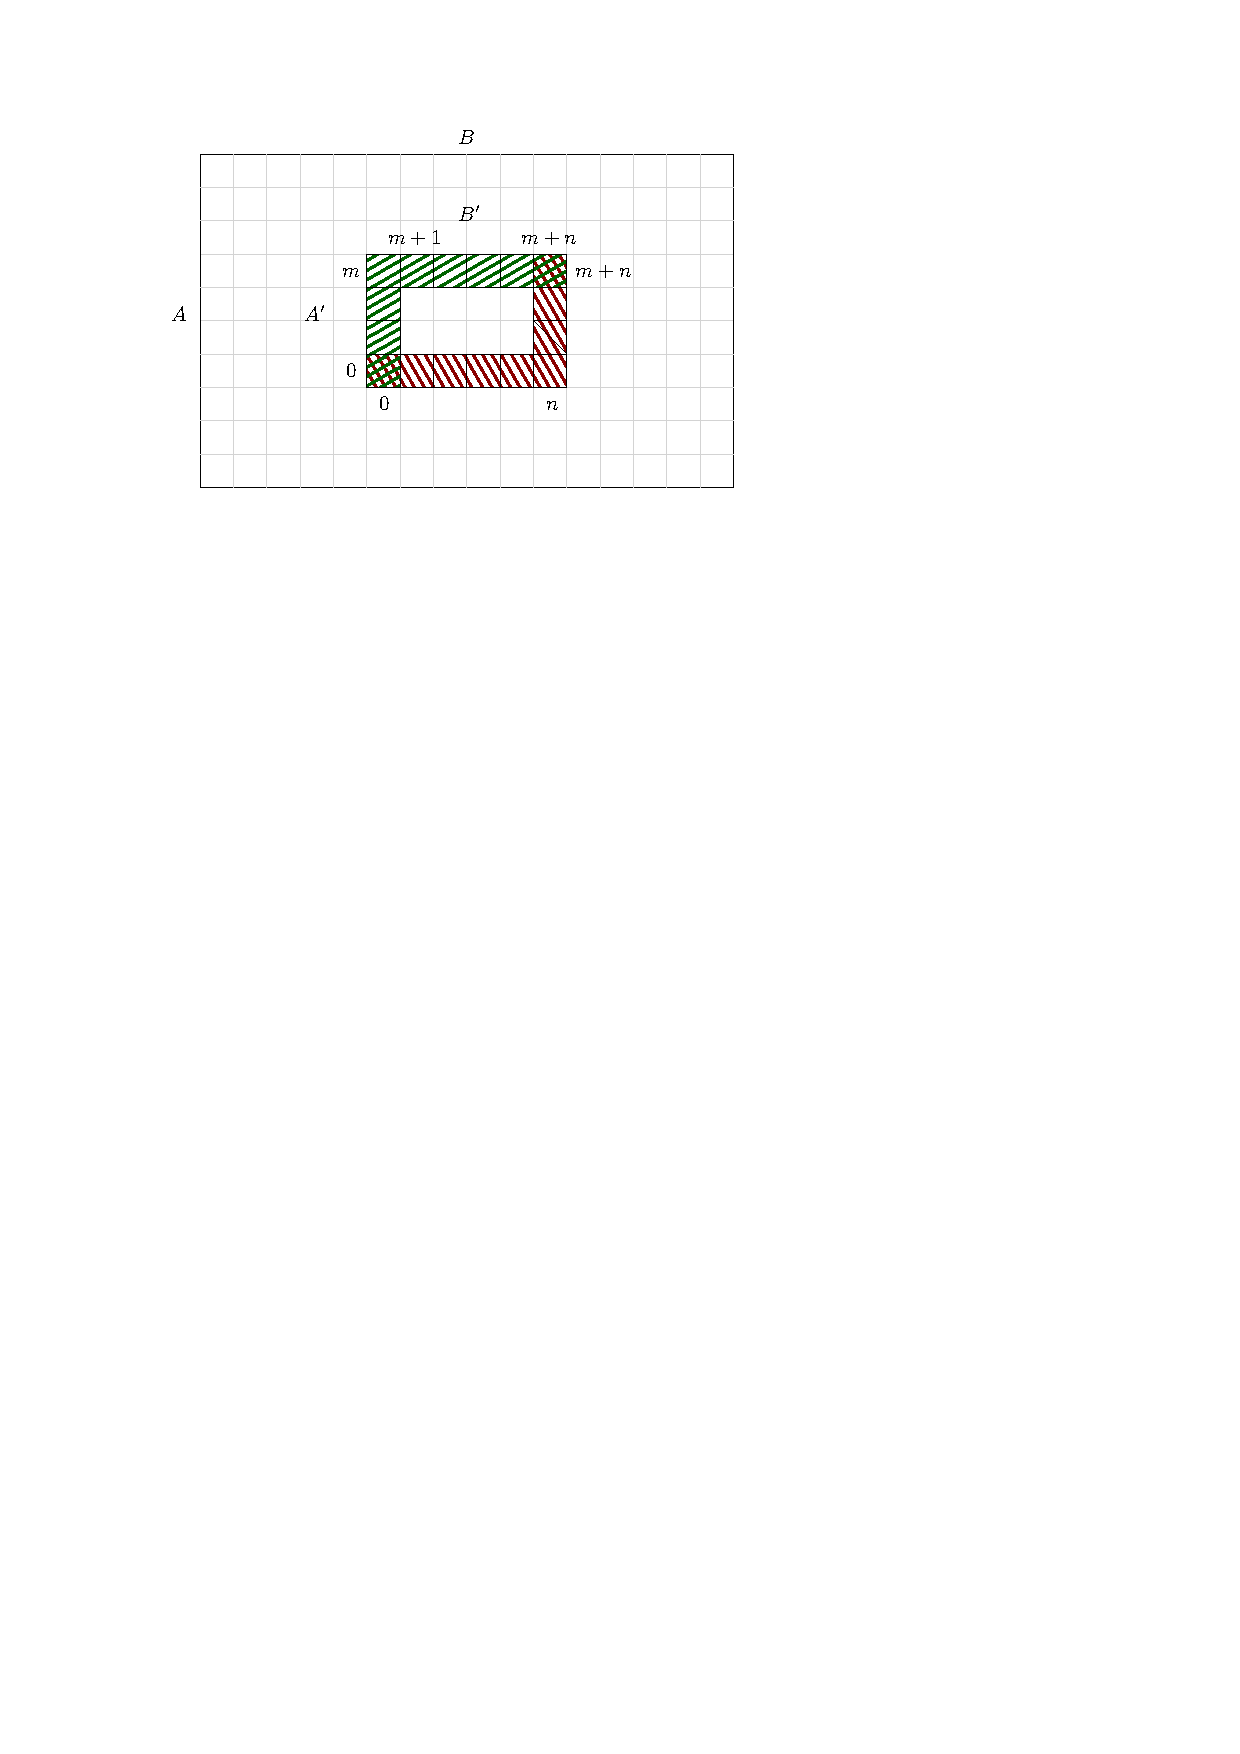
\includegraphics[width=\textwidth]{images/grid-dist}
      \caption{Numbering of inputs (green) and outputs (red) of a $\DIST$-table.}
    \end{subfigure}
    %
    \begin{subfigure}{0.45\textwidth}
      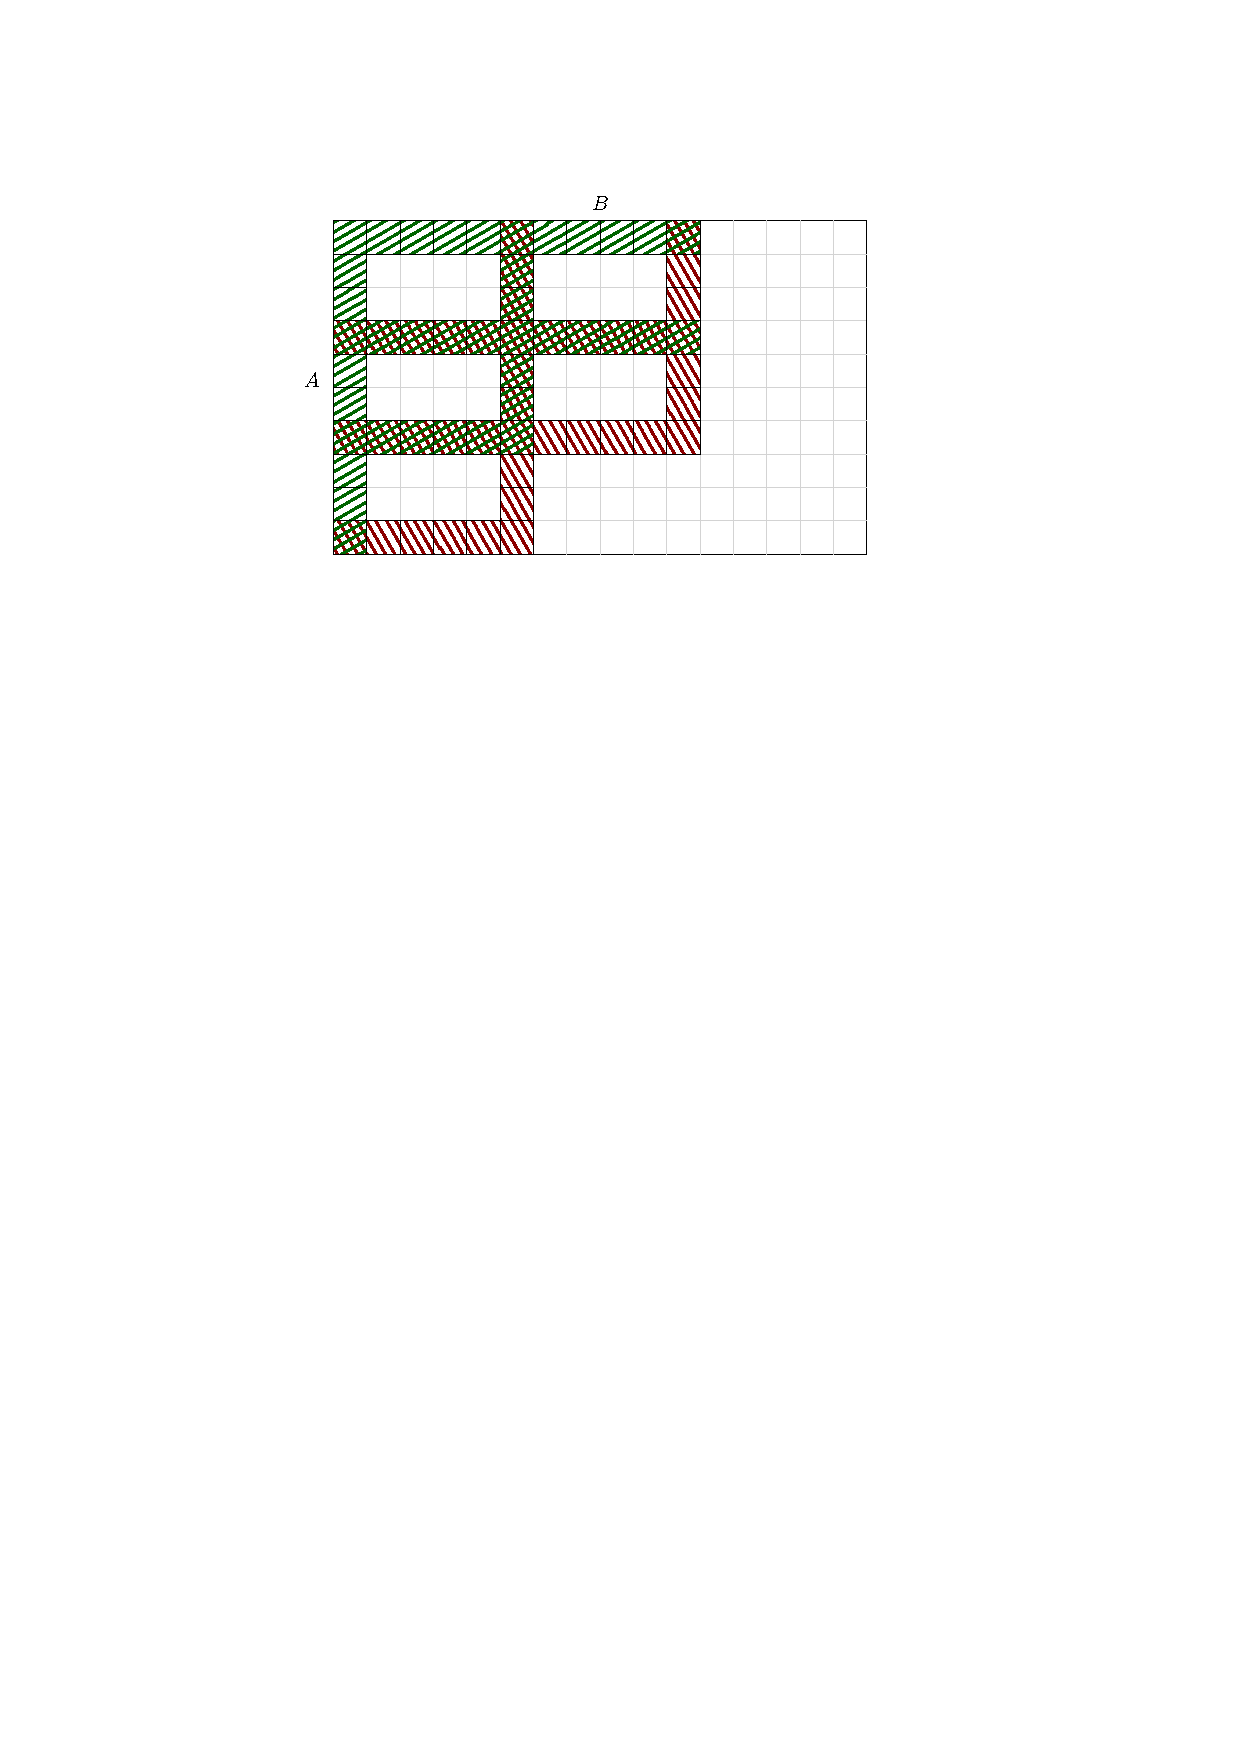
\includegraphics[width=\textwidth]{images/grid-dist-2}
      \caption{How $\DIST$ tables fit together.}
    \end{subfigure}
    \caption{Illustration of $\DIST$ tables.}
    \label{fig:defn-dist-table}
  \end{figure}
\end{mydef}

In order for this technique to work, it is required that the edit distance reduces to the LCS problem with only a constant overhead in time and space consumption. The reduction is given in \cite[p. 71]{DBLP:journals/corr/abs-0707-3619} where it is called the \textit{blow-up technique}.

\subsection{Blow-up technique}
The idea is to “blow-up” the input strings by a constant fraction by inserting special characters, which in a suitable way will relate the length of the LCS of the transformed strings to the edit distance of the original input strings.

The transformation is as follows: All symbols $a \in \Gamma$ in the input strings are transformed to $a\$$, where $\$ \not\in \Gamma$. Denote the transformed strings by $A^{\$}$ and $B^{\$}$. In order to argue that this works, one can consider the possible edit distance operations and show how these can be emulated by computing the LCS on the transformed strings. The cases are illustrated in \cref{fig:blow-up:edit-dist-cases}.

\begin{figure}[!htb]
  \centering
  \begin{subfigure}{0.9\textwidth}
    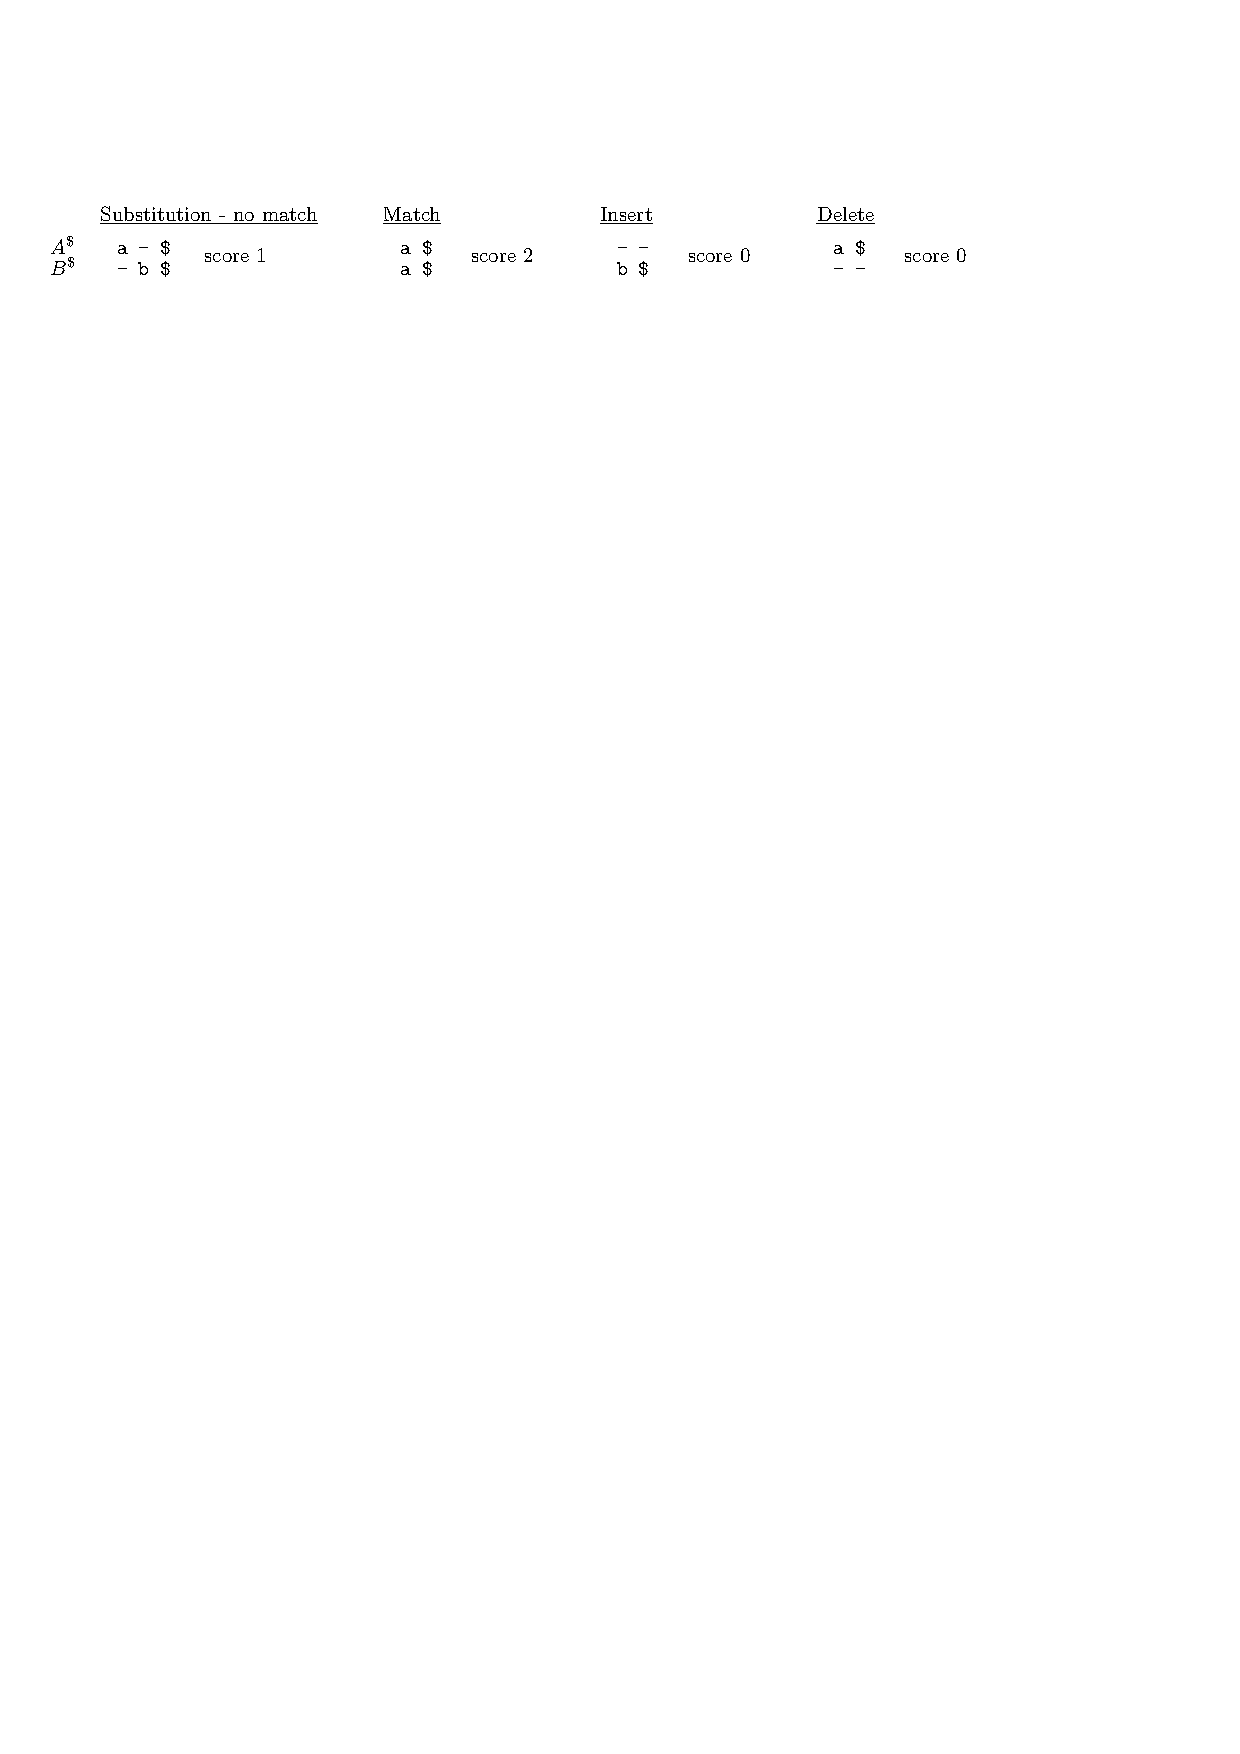
\includegraphics[width=\textwidth]{images/blow-up-edit-dist-cases}
    \caption{Cases that corresponds to edit distance operations.}
    \label{fig:blow-up:edit-dist-cases}
  \end{subfigure}
  %
  \begin{subfigure}{0.8\textwidth}
    \centering
    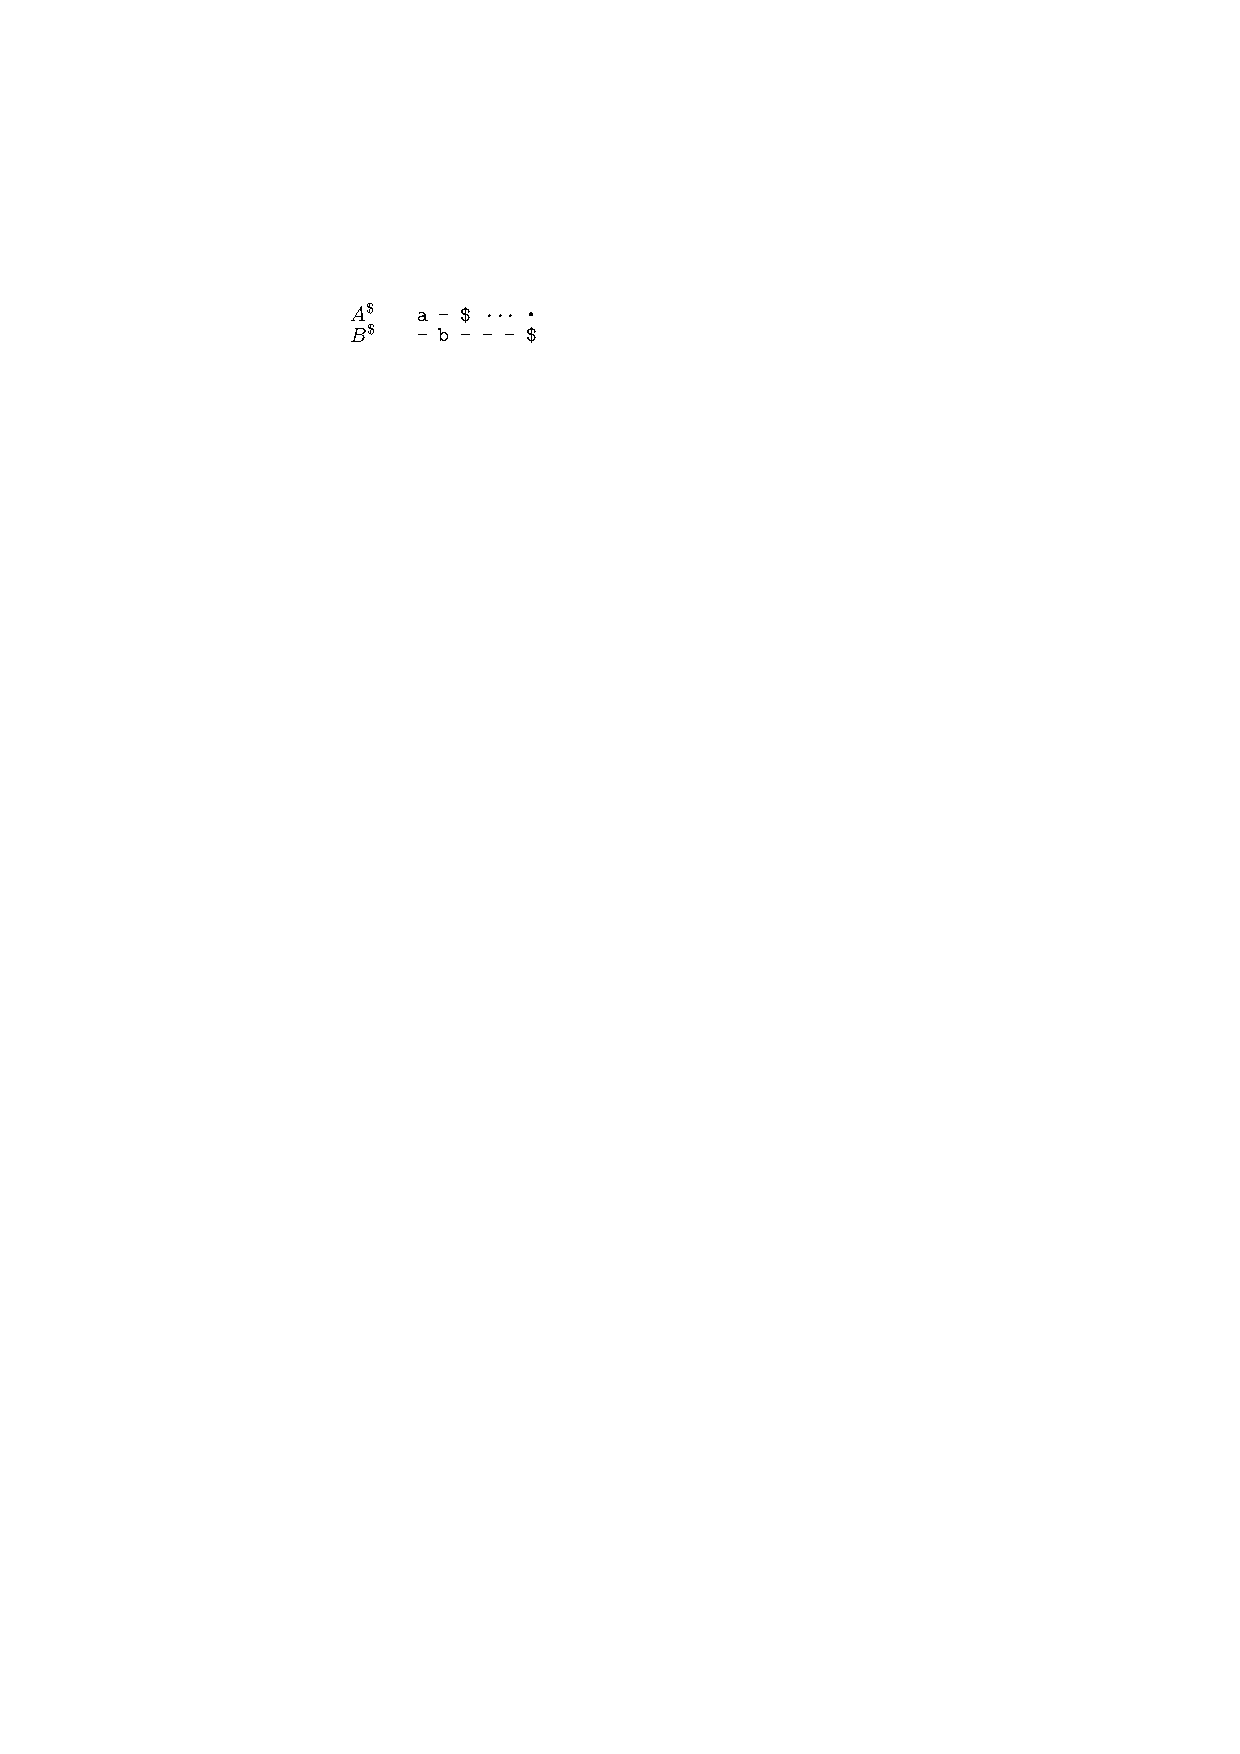
\includegraphics[width=0.2\textwidth]{images/blow-up-not-possible-case}
    \caption{Case that is not possible in longest common substring.}
    \label{fig:blow-up:not-possible}
  \end{subfigure}
  \caption{Possible cases for aligning two transformed strings in the longest common substring world.}
\end{figure}%

Notice that it is not possible to create a longest common substring using other matching strategies than the ones shown in \cref{fig:blow-up:edit-dist-cases}. The only ones that are omitted are cases all similar to the matching shown in \cref{fig:blow-up:not-possible}, but these cases can always be improved by matching the $\$$'s and hence these matchings can not be in the longest common substring.

Due to the scorings of the possible cases in \cref{fig:blow-up:edit-dist-cases}, it can be verified that
\[
  \EditDist(A, B) = n + m - lcs(A^{\$}, B^{\$}),
\]
by considering how the alignment relates for the different cases. The $n + m$ part denotes the worst-case cost of a edit distance alignment of the original strings. For every match operation in the LCS string as depicted in \cref{fig:blow-up:edit-dist-cases}, the edit distance alignment can be changed to match these symbols leading to a reduction of the cost by $2$. For the substitution without a match, only a singe gap is avoided meaning that the edit distance cost should be reduced by $1$. This is also what happens by \cref{fig:blow-up:edit-dist-cases}. For the insertion and deletion cases it also follow that their cost reduction correspond to their LCS scores.

This approach results in the strings becoming a factor of $2$ longer. For the simple $O(N^2)$ implementation of the LCS algorithm, this would result in a factor of $2^2 = 4 = O(1)$ slow down. However, for the compression based algorithm, the penalty will not be as severe, since the blown up strings will compress well. This follows from, and also gives an algorithm for performing the blow-up: Every terminal in the SLP (of which there are $|\Gamma|$) is replaced by a non-terminal producing the original terminal and a new terminal producing the $\$$ symbol. This results in only $|\Gamma| + 1$ new productions being added to the SLP encoding of the string.

\subsection{Selecting SLP productions}
\label{sec:algorithm:select-productions}
In order to be able to save time, the idea is to pre-compute DIST tables based on the productions in the SLPs, such that reused productions means that fewer DIST tables have to be precomputed. There is not enough time to compute DIST tables for all productions. Instead, the SLPs will be chopped into blocks corresponding to productions, covering the entire string, where each block derives strings of length $O(x)$ for some $x \in \mathbb{N}$. $\DIST$ tables will then be precomputed for these blocks.

Both of the input SLPs will be blocked in the same way. The blocking process applied is from \cite[Section 4]{DBLP:journals/corr/abs-1004-1194} and consists of two steps. First what will be known as \textit{key productions} are selected and then productions in between the key productions are selected.

\begin{figure}[!htb]
  \centering
  \includegraphics[width=14cm]{images/key-production-example}
  \caption{Illustrates how productions are selected that cover the entire string for the SLP given in \cref{fig:slp-example} and using $x = 3$.}
  \label{fig:key-production-selection}
\end{figure}

The key productions are identified by traversing the unfolded SLP bottom up. If the string derived by the current production has length less than $x$ it is annotated with an associated string, which in this case is the string it derives\footnote{In practice the actual associated string is not needed, but only the length of the associated string. Therefore only the length of the associated string is stored in the implementation.}. If the length is greater than $x$ and both its children have length less than $x$, the production is marked as a key production and its associated string is set to the string it derives. Otherwise no action is taken. An illustration of how key productions are selected can be seen on \cref{fig:key-production-selection}.

All the selected key productions cover some part of the string. In order to cover the rest of the input string extra productions need to be added. These are called second type productions. In order to find these, the path between two adjacent key productions is traversed. This is done by first finding the lowest common ancestor of the two key productions, and then traversing the paths from both of the key productions to the lowest common ancestor bottom up. Notice that all productions hanging from the traversed paths must all have derived strings with length less than $x$ since they would be marked as key productions otherwise. See \cref{fig:slp-2nd-type} for an illustration.

\begin{figure}[!htb]
  \centering
  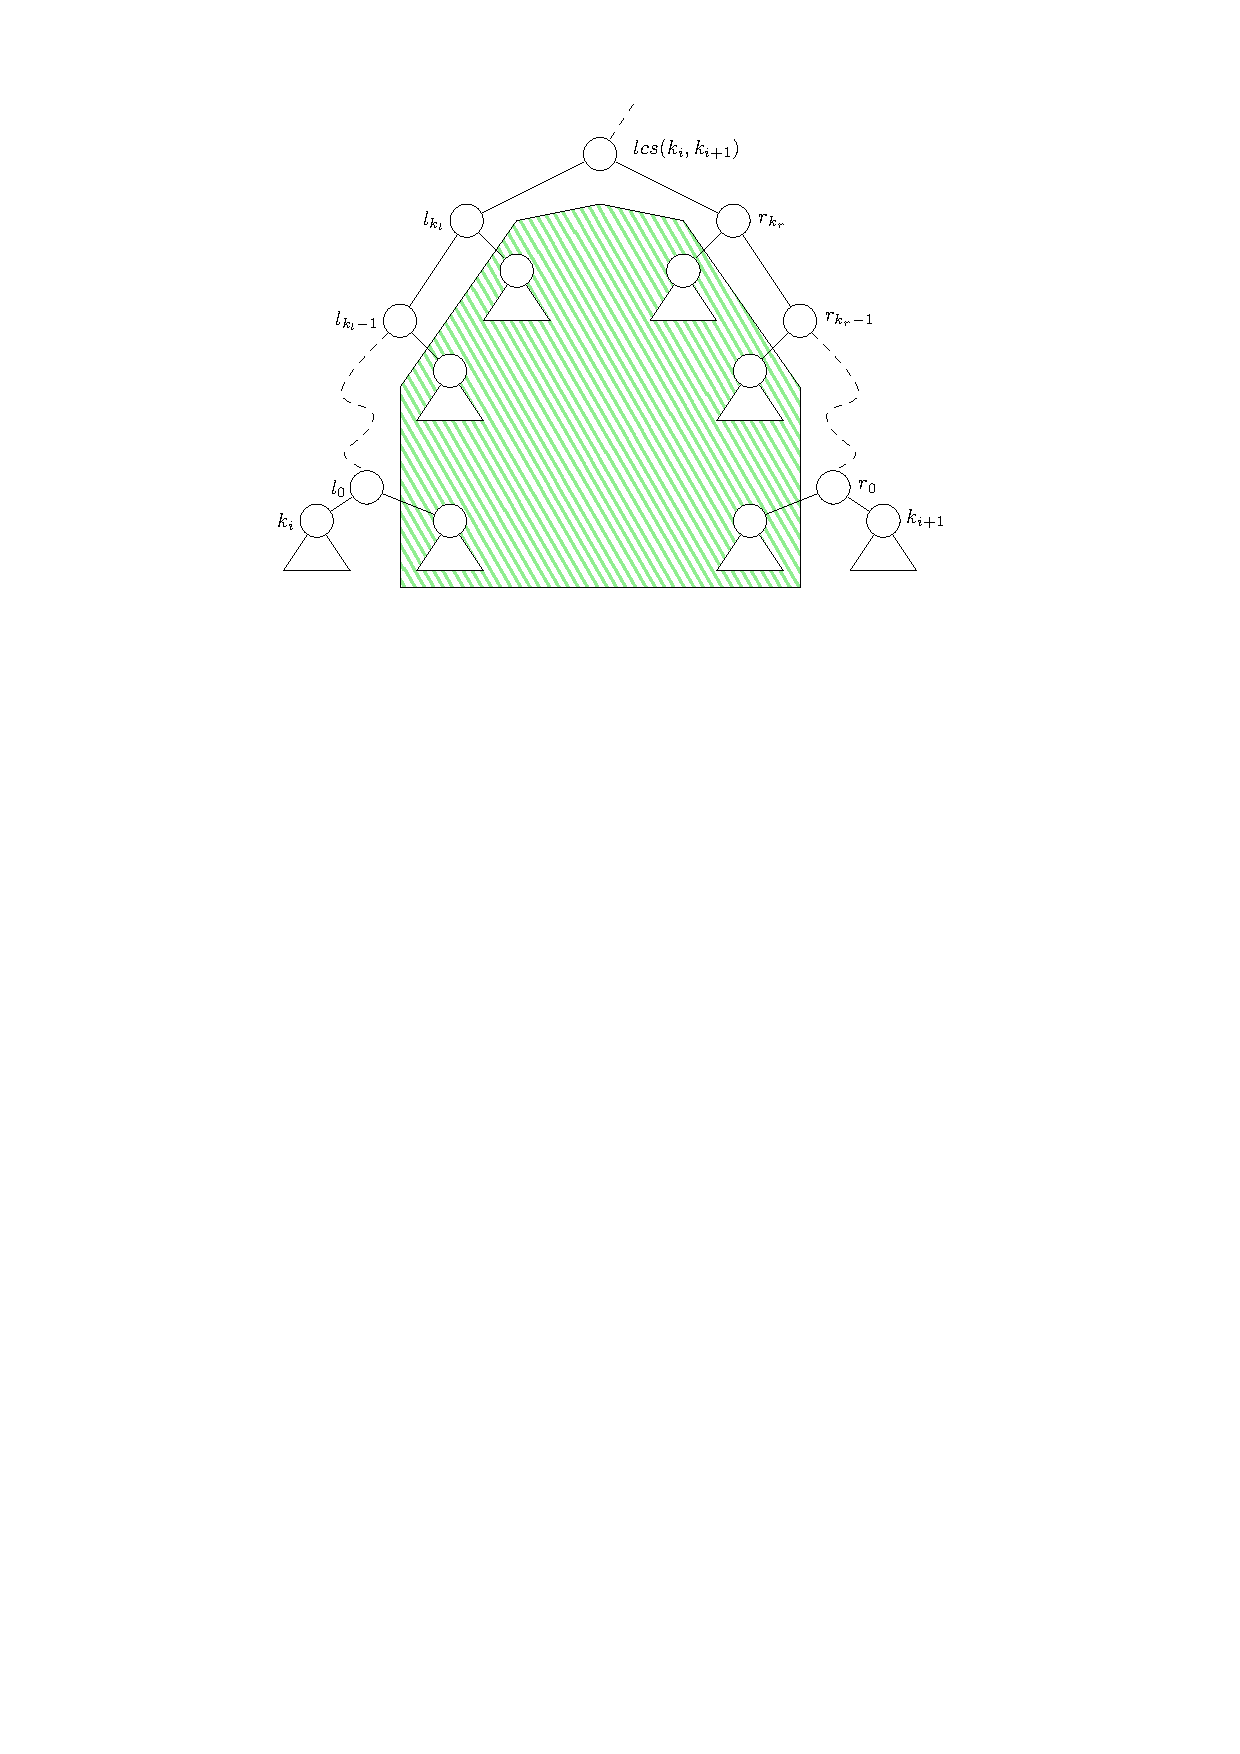
\includegraphics[width=10cm]{images/slp-2nd-type}
  \caption{An illustration of how production of the second type relates to the key productions $k_i, k_{i+1}$. The productions inside the green areas span the part of the string that is not covered by the key productions. The productions on the path between the two key productions are labeled by $l_0, \dots, l_{k_l}$ and $r_0, \dots, r_{k_r}$.}
  \label{fig:slp-2nd-type}
\end{figure}

When traversing the left path, the strings derived by the productions hanging to the right are associated to the productions on the path. These strings are merged bottom up into strings of length less than $2x$. This is done by successively merging the string starting from the bottom. If the current string generated has length less than $x$, the current string is propagated to the next production and the productions are linked. If the current string is of length greater than $x$, the current production is selected and its associated string is the current propagated string. This process is done analogously for the right path.

There is a special case with the beginning and end of the string, as there are not necessarily a key production spanning the first and the last part of the string. However, these cases can be accommodated by the path traversing algorithm applied to the left path for the beginning and one right path for the end.

By this process, all the selected productions will span the entire input string and they are all associated with strings of length $O(x)$.

Due to the bottom up nature of the selection process, a repeated production in two parts of the string will result in the same selected productions. This is very important in order to obtain the desired speedup, since DIST tables are precomputed for all the selected productions. Therefore, reducing the number of different selected productions yields a time improvement when building the DIST tables.

One technical detail to notice for the above approach to work directly, is that a production is only associated with one unique string, even through a production may occur several times in the unfolded SLP. Due to the bottom up selection, this is clear for the key productions. For the second type it follows since the same key productions are selected in different parts of the strings, resulting in the paths between the key productions being unique, so that they always produce the same result.

\subsection{Building the DIST repository}
\label{sec:algorithm:building-DISTs-overview}
In the previous step it was described how to select the productions for which the $\DIST$ repository should be built. This section will focus on how the $\DIST$ repository is constructed. More specifically the $\DIST$ repository contains a $\DIST$ table for every pair of selected productions in the two SLPs. In other words, let $P_\mathcal{A}$ and $P_\mathcal{B}$ denotes the selected productions in respectively the SLPs $\mathcal{A}$ and $\mathcal{B}$. Then the $\DIST$ repository contains a $\DIST$ table $\DIST_{a,b}$ for all $a \in P_\mathcal{A}, b \in P_{\mathcal{B}}$.

The $\DIST$ tables will be constructed by means of recursively merging $\DIST$ tables for sub-productions of the selected productions. The base case for a pair of terminals is not explicitly described in this section, but will follow directly from definition once the concrete representation of the $\DIST$ tables have been described in \cref{lemma:H-permutation-representation}.

The previously described production selection process, divides the selected productions into two types. The following describes how to handle the two cases.
\\
\begin{description}
  \item[Key productions] A key production is always associated with the string that the production derives. Therefore assume the DIST table for two key productions $a \in P_{\mathcal{A}}$ and $b \in P_{\mathcal{B}}$ should be built. Name the children of the two productions by $a_L, a_R$ and $b_L, b_R$ as illustrated on \cref{fig:distrepo-key}.
  
  \begin{figure}[h!]
    \centering
    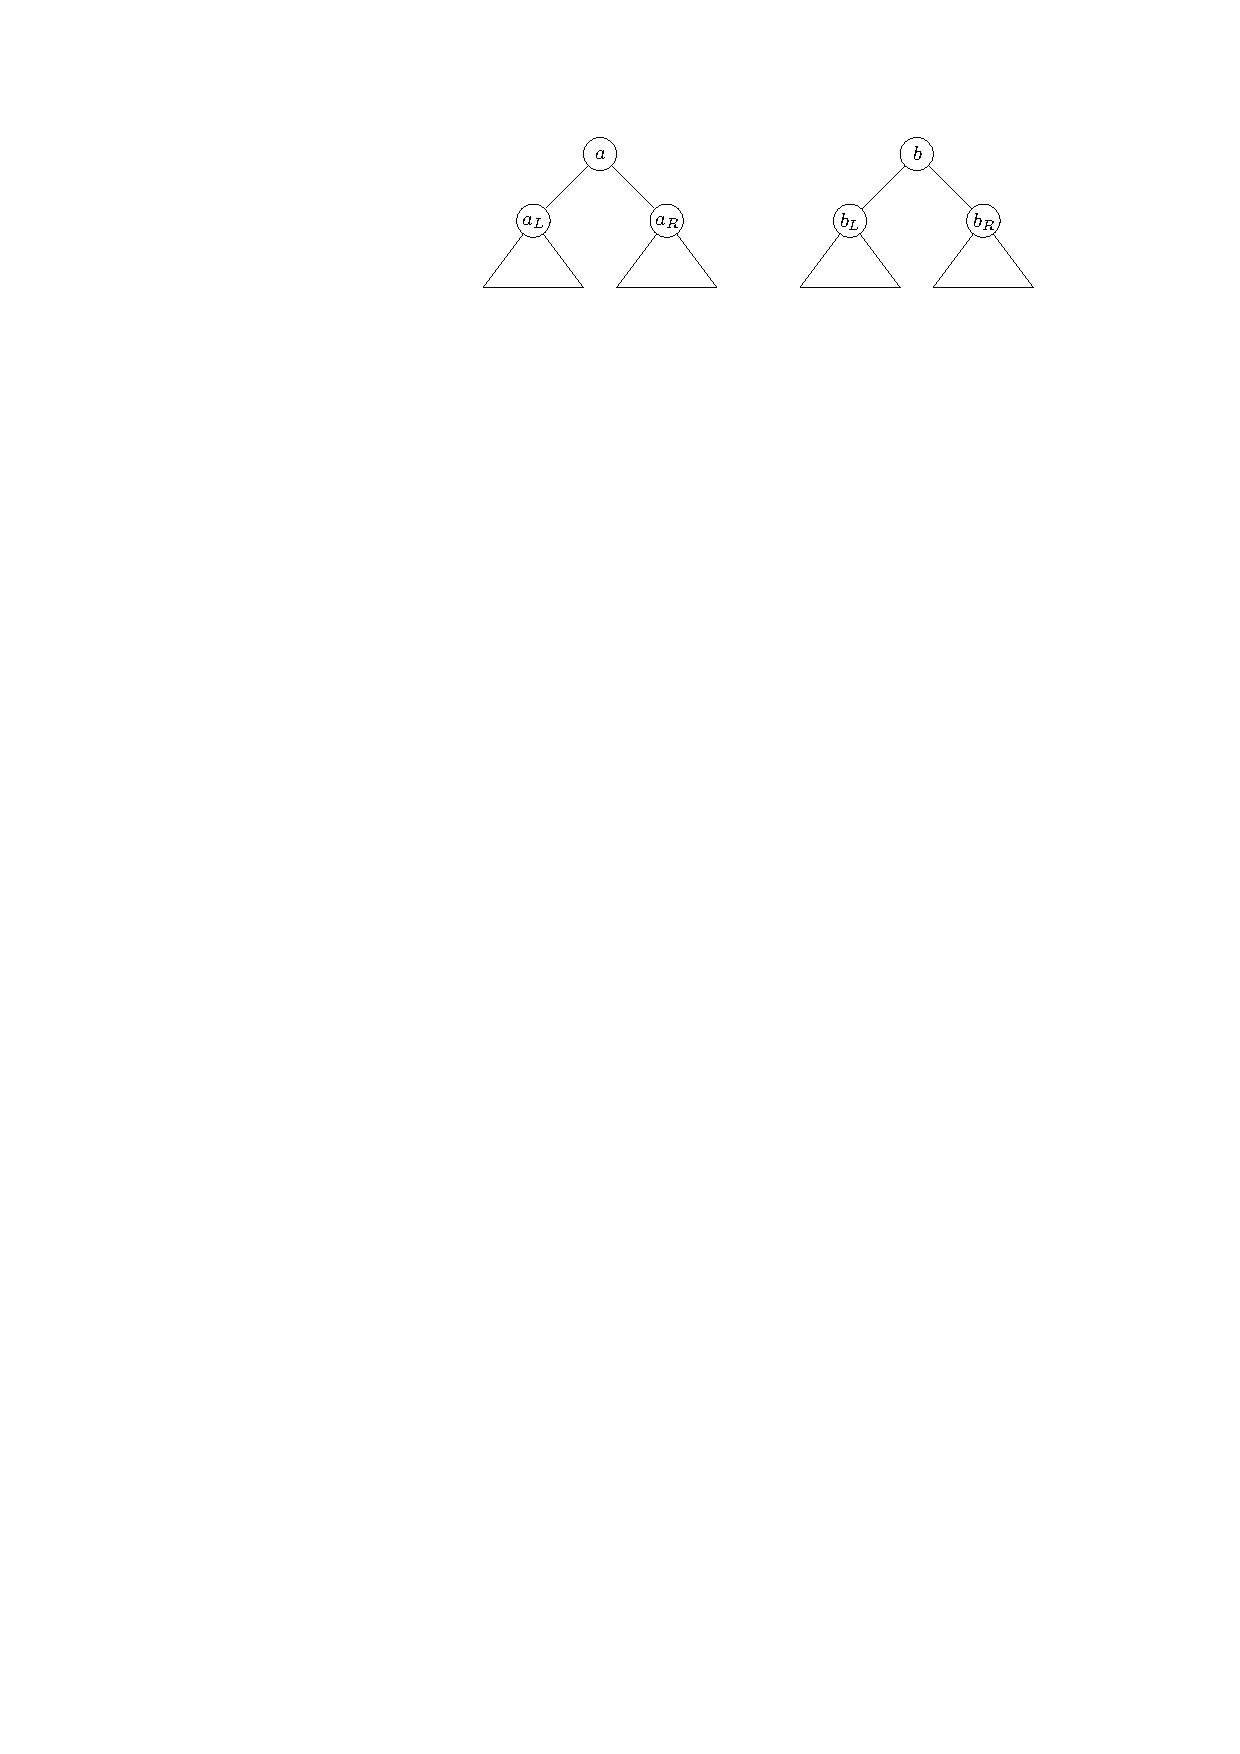
\includegraphics[width=10cm]{images/distrepo-key}
    \caption{Illustration of a key production.}
    \label{fig:distrepo-key}
  \end{figure}
  
  The DIST table is constructed by first recursively constructing the DIST tables for all combinations of the children, ie. $(a_L, b_L), (a_L, b_R), (a_R, b_L)$ and $(a_R, b_R)$. Then the DIST from $a$ and $b$ can be obtained by merging as shown in Figure~\ref{fig:compression:dist:merge}. For now merging of $\DIST$ tables will be assumed to be a black box. The details of the merging process will be given in \cref{sec:merging-dists}.
  \begin{figure}[h!]
    \centering
    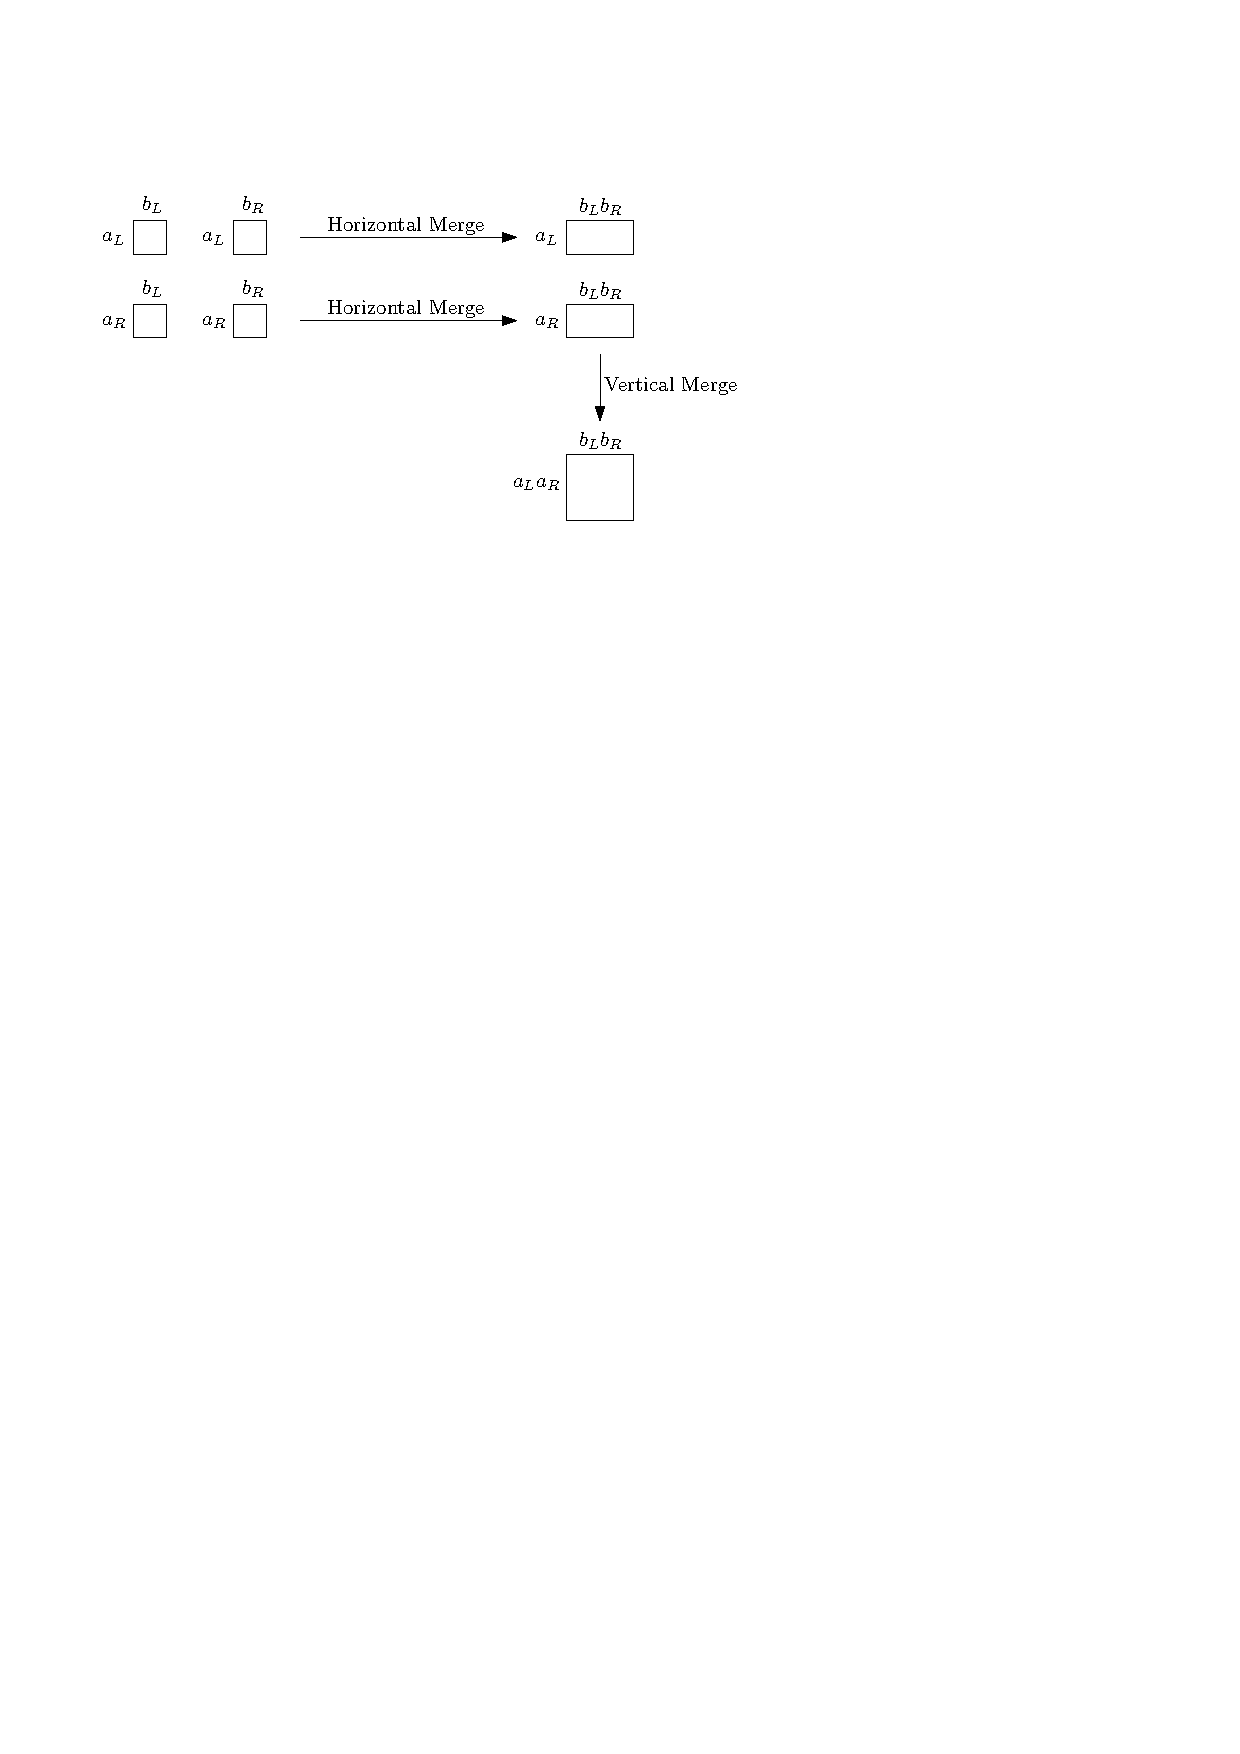
\includegraphics[width=10cm]{images/dist_merge}
    \caption{Merging phases of DIST tables from the children to obtain the DIST for the concatenated strings.}
    \label{fig:compression:dist:merge}
  \end{figure}

  \item[Second type of selected productions] For this type of productions the associated string is not the string that the production derives. Instead the associated string is the right (or left) child, possibly combined with the right (or left) child of its left (or right) child. A graphical illustration is given on \cref{fig:distrepo-2nd} where the production is on a left path. The right path case is symmetric and is not included.

  \begin{figure}[h!]
    \centering
    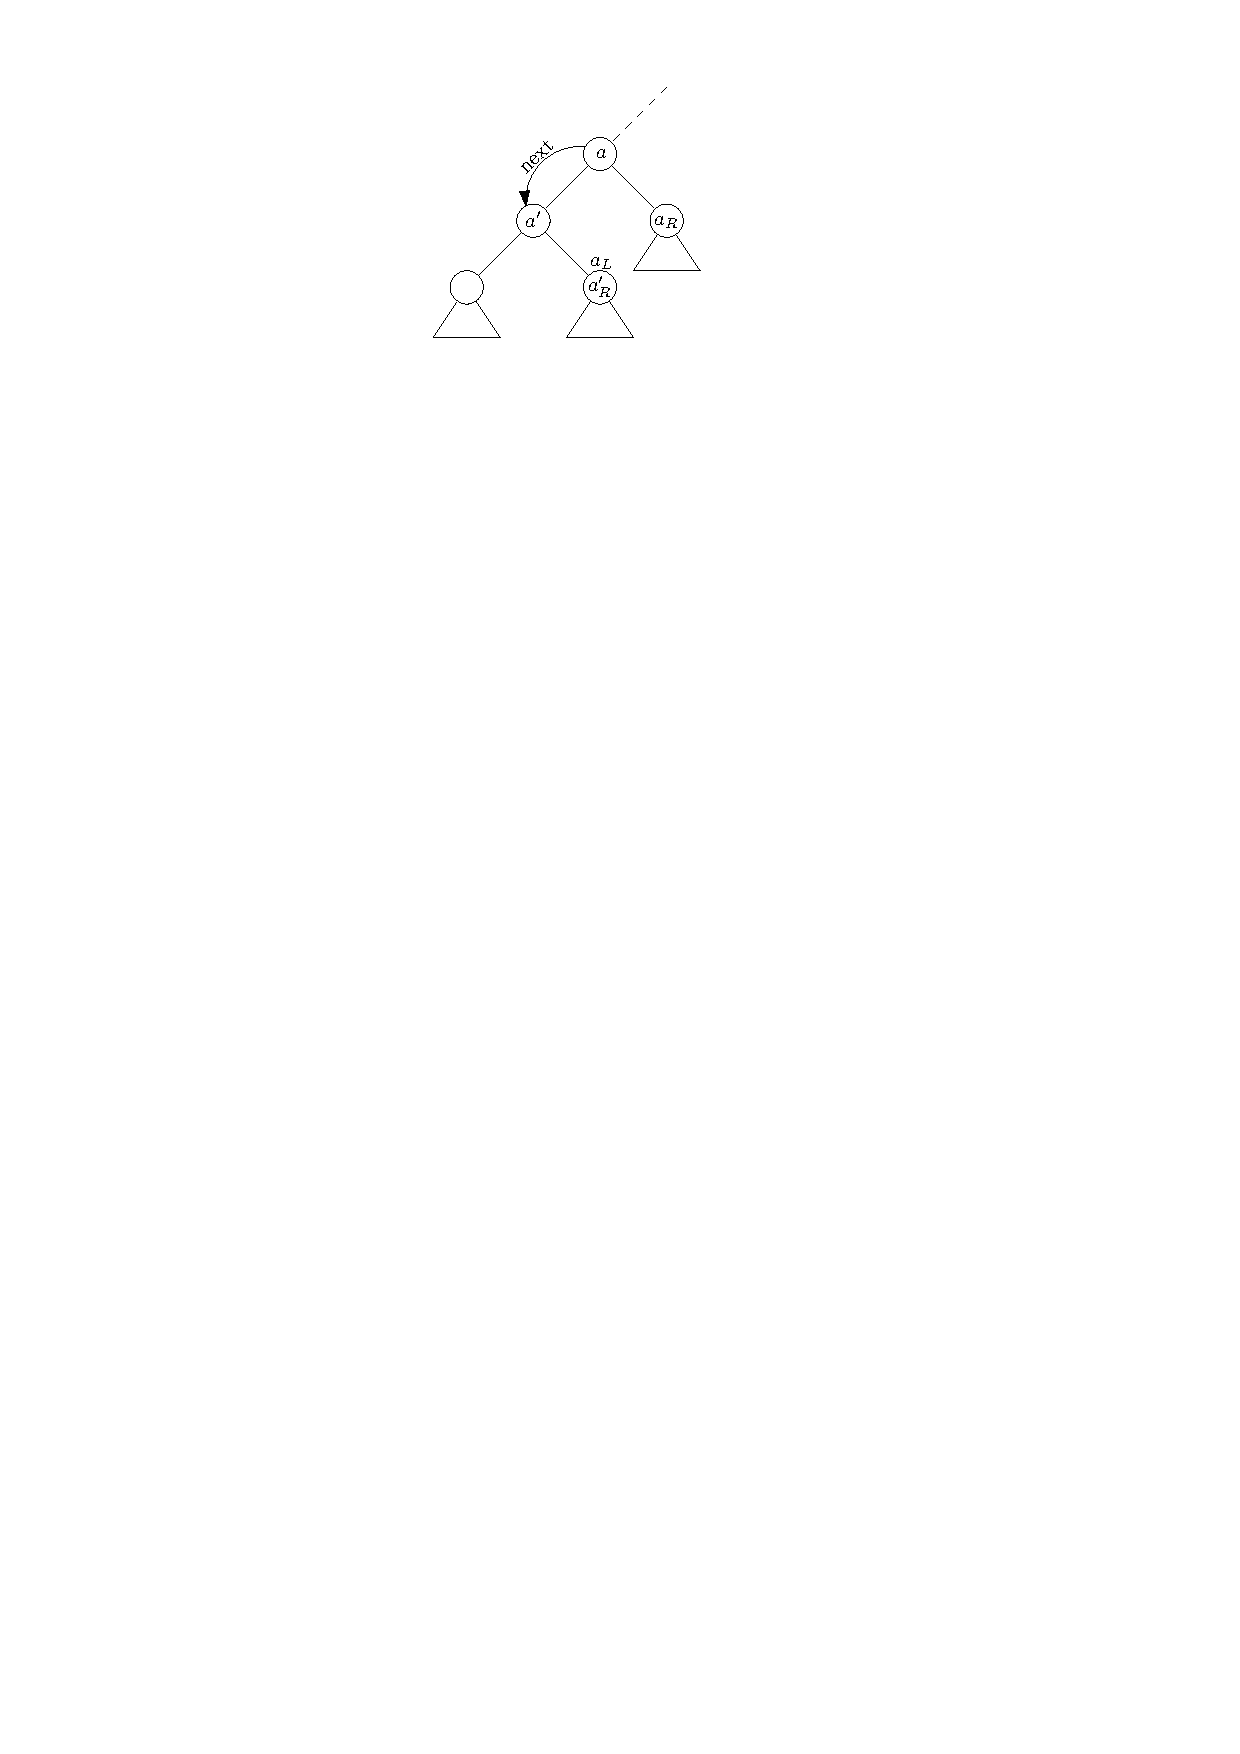
\includegraphics[width=5cm]{images/distrepo-2nd}
    \caption{Illustration of how a production of the second type is handled.}
    \label{fig:distrepo-2nd}
  \end{figure}

  By adopting the notation of $a_L$ and $a_R$ from \cref{fig:distrepo-key}, and using the appropriate definitions of $b_L, b_R$ from the type of the $b$ production, the merging process of \cref{fig:compression:dist:merge} gives the desired result.
  \enlargethispage{\baselineskip}
\end{description}
Since the number of productions is bounded by $O(n^2)$, memorization can be used in combination with the above procedure to construct the $\DIST$ repository in time $O(n^2 M(x))$, where $M(x)$ denotes the time for merging two $\DIST$ tables. As will be seen in \cref{sec:merging-dists} the merging can be done in time $M(x) = O(x\log{x})$, leading to a total running time of $O(n^2x\log{x})$ for computing the DIST repository.

\subsection{Filling out the dynamical programming table}
\label{sec:algorithm:filling-grid-overview}
The dynamical programming table is filled from top to bottom, left to right. This is done by applying the $\DIST$ tables one by one using the selected productions. The inputs of the $\DIST$-table to be applied is kept in memory by storing two columns of the dynamic programming grid and $O(x)$ of a row. By using \cref{defn:dist-table} it is easy to see that the outputs of the $\DIST$ table can be computed as
\begin{equation}
  \label{eqn:dist-application}
  O[j] = \min_i \{ I[i] + \DIST[i, j] \},
\end{equation}
since the $\DIST$ table stores the shortest path from input $i$ to output $j$. Evaluating the above formula directly for every input takes $O(x^2)$ time, which is too much.

However, by representing the $\DIST$ tables in a clever way, the time required to evaluate \cref{eqn:dist-application} can be reduced to $O(x)$. This algorithm is described in \cref{sec:applying-a-dist-table}. Therefore, the total time for filling out the grid becomes $O\left( \frac{N^2}{x^2}x \right) = O\left( \frac{N^2}{x} \right)$.

\subsection{Combining the two steps}
\label{sec:combining-the-two-steps}
In order to reduce the running time, the idea is to asymptotically balance the time used to compute the $\DIST$ repository and to fill out the grid. In order to do this, define $f = \frac{N}{n}$ to be the inverse compression ratio of the input strings.

The size parameter for the SLP blocking $x$ is defined to be $x = \frac{f}{\sqrt{\log{f}}}$. This choice results in the $\DIST$ repository taking
\begin{align*}
  O(n^2 x\log{x})
    &= O\left( n^2 \frac{f}{\sqrt{\log{f}}} \log\left( \frac{f}{\sqrt{\log{f}}} \right) \right)
    = O\left( Nn \frac{1}{\sqrt{\log{\frac{N}{n}}}} \log\left( \frac{N/n}{\sqrt{\log{\frac{N}{n}}}} \right) \right) \\
    &= O\left( Nn \frac{1}{\sqrt{\log{\frac{N}{n}}}} \left( \log{\frac{N}{n}} - \log{\sqrt{\log{\frac{N}{n}}}} \right) \right)
    = O\left( Nn\sqrt{\log{\frac{N}{n}}} \right)
\end{align*}
time to build. The grid can be filled in time
\[
  O\left(\frac{N^2}{x}\right)
    = O\left( \frac{N^2}{\frac{f}{\sqrt{\log{f}}}} \right)
    = O\left( \frac{N^2 \sqrt{\log{f}}}{f} \right)
    = O\left( Nn\sqrt{\log{\frac{N}{n}}} \right).
\]
Since the SLP construction algorithm runs in time $O(N\log{N})$, the combined running time for the combined algorithm becomes $O\left( Nn\sqrt{\log{\frac{N}{n}}} \right)$. In the big-O notation this running time is always superior to $\Theta(N^2)$ which is the time required by the simple algorithm.

The theoretical combined running time from this section remains valid when $f$ and $x$ are multiplied by arbitrary constants. Call these constants respectively $\ffactor$ and $\xfactor$ such that $f = \ffactor \cdot \frac{N}{n}$ and $x = \xfactor \cdot \frac{f}{\sqrt{\log{f}}}$. It is likely that changing these constants will have a big influence on the actual running time of the algorithm. Therefore the effect of different choices have been examined in \cref{sec:benchmark:slp-partition-factors}.

\section{Representing $\DIST$ tables}
As mentioned in the previous section, representing the $\DIST$ tables in a succinct way is crucial in order to obtain the desired running time.

Given two strings $A$ and $B$, a succinct representation of the LCS $\DIST$ tables should be constructed. By \cref{defn:dist-table} it is known that
\[
  \DIST_{A,B}[i, j] = \left\{
    \begin{array}{ll}
      lcs(\substr{A}{m - i}{m}, \substr{B}{0}{j})             & \text{if } i < m, j < n \\
      lcs(A, \substr{B}{i - m}{j})                            & \text{if } i \geq m, j < n \\
      lcs(\substr{A}{m - i}{m - (j - n)}, B)                  & \text{if } i < m, j \geq n \\
      lcs(\substr{A}{0}{m - (j - n)}, \substr{B}{i - m}{n})   & \text{if } i \geq m, j \geq n
    \end{array}
  \right. ,
\]
that is, the $\DIST$ can be summarized as the LCS between all prefix-suffix pairs of the two strings $A$ and $B$.
Notice that a $\DIST$ table is not well-defined for $i > j + m$ and $j > i + n$ since it corresponds to non-existing paths in the dynamic programming table. In all following calculations and statements these invalid index combinations should simply be considered as statements without any information.

A different way of describing the LCS between these prefix-suffix pairs, is by the following definition.

\begin{mydef}[\refbook{p.-48}{Definition 4.8}]
  \label{def:H-table}
  Let $\str{A}{0}{m}$ and $\str{B}{0}{n}$ be strings, then for $i, j \in \{ 0, \dots, m + n \}$ define
  \[
    H_{A,B}(i, j) := \begin{cases}
                        j - (i - m)                         & \text{if j < i - m} \\
                        lcs(A, \substr{?^mB?^m}{i}{j + m})  & \text{o/w}
                      \end{cases}
  \]
  where $? \not\in \Gamma$ denotes a wildcard character matching all other symbols.
\end{mydef}
The first case in the $H_{A,B}$ definition is introduced because these entries in the corresponding $\DIST$ table are not well-defined. The values for these entries of the $H$-table are simply chosen to make everything work out as they should in order to make the $H$-tables easy representable. In almost all the following calculations it has been chosen not to include this case as it is straight forward that the choice will work. This is due to the definition of the $\Sigma$-operator and that unit-Monge matrices are closed under the minimum distance product.

When it is clear which strings a $\DIST$- or $H$-table are based upon they may be omitted from the notation in order to simplify the look of the expressions. I.e. $\DIST_{A,B}$ may be written as $\DIST$ and $H_{A,B}$ as $H$.

The precise correspondence between a $H$-table as defined in \cref{def:H-table} and a $\DIST$ table as defined by \cref{defn:dist-table} is given by the following lemma.
\begin{lemma}[\refbook{p.-48}{mentioned but not proved}]
  \label{lemma:dist-H-relation}
  Given a $\DIST$ table $\DIST$ and a $H$-table $H$ on the same strings $A$ and $B$, they are connected by the relation
  \[
  DIST[i, j] = H(i, j) + \left\{
    \begin{array}{ll}
      i - m             & \text{if } i < m, j < n \\
      0                 & \text{if } i \geq m, j < n \\
      (i - m) + (n - j) & \text{if } i < m, j \geq n \\
      n - j             & \text{if } i \geq m, j \geq n
    \end{array}
  \right. .
  \]
  \begin{proof}
    The lemma follows almost directly by the definition of the DIST, $H$-table and $lcs$ function, by splitting the claim up into the four different cases of the statement.
    \begin{description}
      \item[\circled{1}] For $i \in \{0, \dots, m\}, j \in \{0, \dots, n\}$,
       \begin{align*}
         H(i, j) &= lcs(A, \substr{?^mB?^m}{i}{j + m}) = lcs(A, ?^{m - i}\substr{B}{0}{j}) \\
                 &= (m - i) + lcs(\substr{A}{m - i}{m}, \substr{B}{0}{j}) = \DIST[i, j] + m - i
       \end{align*}

      \item[\circled{2}] For $i \in \{m, \dots, m + n\}, j \in \{0, \dots, n\}$,
        \[
          H(i, j) = lcs(A, \substr{?^mB?^m}{i}{j + m}) = lcs(A, \substr{B}{i - m}{j}) = \DIST[i, j]
        \]

      \item[\circled{3}] For $i \in \{0, \dots, m\}, j \in \{n, \dots, n + m\}$,
        \begin{align*}
          H(i, j) &= lcs(A, \substr{?^mB?^m}{i}{j + m}) = lcs(A, ?^{m - i}B?^{j - n}) \\
                  &= (m - i) + (j - n) + lcs(\substr{A}{m - i}{m - (j - n)}, B) \\
                  & = (m - i) + (j - n) + \DIST[i, j]
        \end{align*}

      \item[\circled{4}] For $i \in \{m, \dots, m + n\}, j \in \{n, \dots, n + m\}$,
        \begin{align*}
          H(i, j) &= lcs(A, \substr{?^mB?^m}{i}{j + m}) = lcs(A, \substr{B}{i - m}{n}?^{j - n}) \\
                  &= (j - n) + lcs(\substr{A}{0}{m - (j - n)}, \substr{B}{i - m}{n}) = (j - n) + \DIST[i, j]
        \end{align*}
    \end{description}
  \end{proof}
\end{lemma}
An important property of the $H$-table is that it is almost simple unit-Monge.
\begin{lemma}[\refbook{p.-49}{Theorem 4.10}]
  \label{lemma:H-permutation-representation}
  Given a $H$-table $H$, there exists a permutation matrix $P$ of size $m + n - 1$ such that
  \[
    H(i, j) = j - (i - m) - P^{\Sigma}(i, j).
  \]
  Therefore, the permutation matrix $P$, which can be represented in linear space, encodes the $H$-table, and thereby also the $\DIST$-table.

  \begin{proof}
    Define the following matrix to be a small pertubation of the $H$-table
    \[
      N(i, j) := j - (i - m) - H(i, j).
    \]
    We will prove that $N$ is simple unit-Monge, which directly implies the statement. First it will be shown that $N$ is Monge, that is $N^{\Box} \geq 0$. From the definition of $N$ and $\Box$ it is needed to show that
    \begin{align*}
      &H(i, j + 1) - H(i, j) - H(i + 1, j + 1) + H(i + 1, j) = H^{\Box}(i, j) \leq 0 \\
      \iff &H(i, j + 1) + H(i + 1, j) \leq H(i, j) + H(i + 1, j + 1)
    \end{align*}
    for all $i,j$. By \cref{def:H-table} the adjacent entries of the $H$-table in the above equation correspond to the LCS of a fixed string with a string where a character is possibly extended in both ends. The situation is illustrated in \cref{fig:H-permutation-representation:monge} where the top of the illustration corresponds to the left hand side of the inequality and the bottom corresponds to the right hand side.

    It is clear that the part between $i + 1$ and $j$ will always ensure some fixed contribution to all of the intervals. Now assume that the top contribution is strictly more than two times this fixed contribution. This can happen if it is possible to match an unmatched symbol by introducing cell $i$ or $j + 1$. Notice that if this is the case, then the same can be done for one (or both) of the bottom intervals. Therefore the bottom intervals will always match more than the top intervals, which gives the inequality and thereby the Monge property.
    \begin{figure}[h!]
      \centering
      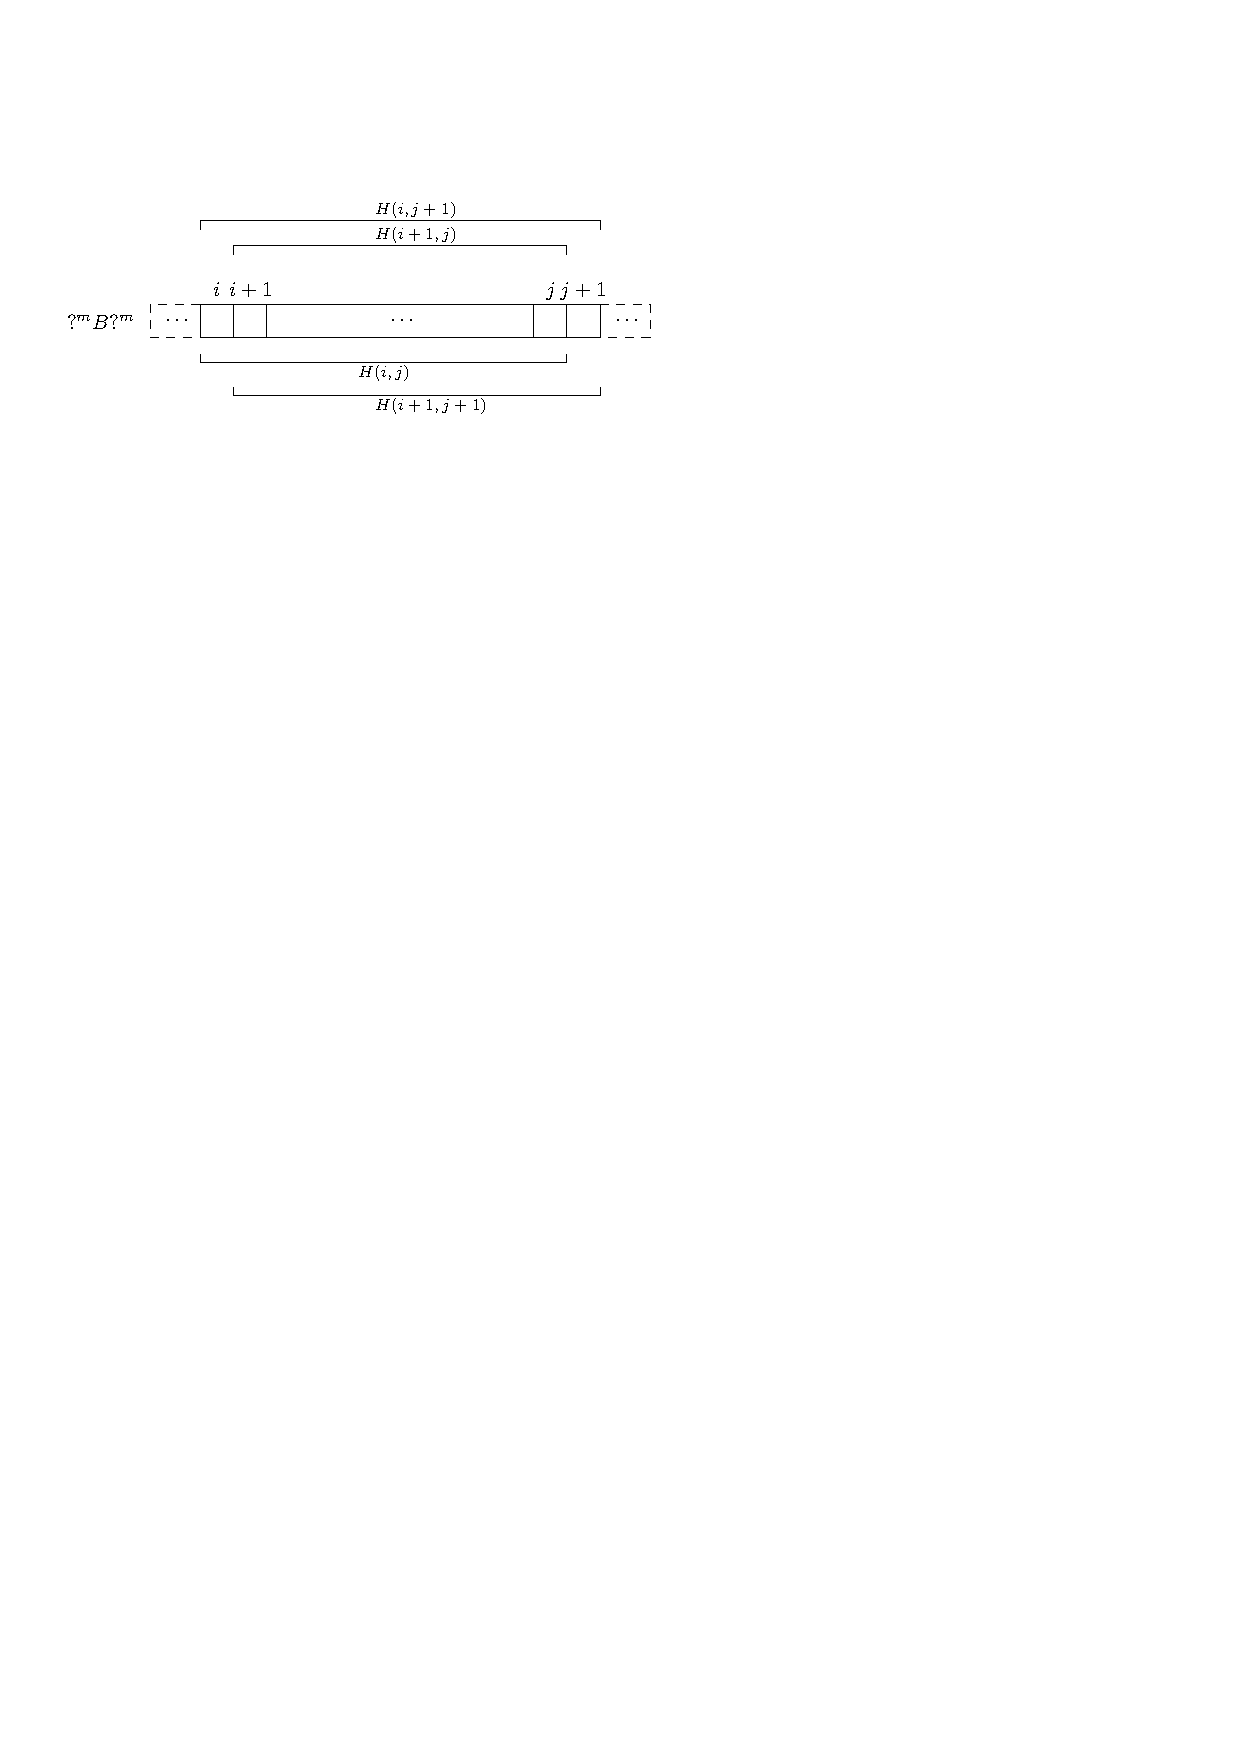
\includegraphics[width=11cm]{images/monge-condition-illustration}
      \caption{Illustration of how the longest common substring extension relates to the Monge property.}
      \label{fig:H-permutation-representation:monge}
    \end{figure}

    Note the following properties about $N$:
    \begin{align*}
      N(i, 0) &= 0 - (i - m) - H(i, j)
        = (m - i) - \begin{cases}
          0 - (i - m)                    & \text{if } i > m \\
          lcs(A, \substr{?^mB?^m}{i}{m}) & \text{o/w}
        \end{cases} \\
        &= (m - i) - (m - i) = 0
    \end{align*}
    \begin{align*}
      N(m + n, j) &= j - ((m + n) - m) - H(i, j) \\
        &= j - n - \begin{cases}
          j - n                                   & \text{if } j < n \\
          lcs(A, \substr{?^mB?^m}{m + n}{j + m})  & \text{o/w}
        \end{cases} \\
        &= (j - n) - (j - n) = 0
    \end{align*}
    Therefore \cref{claim:simple-matrix-characterization} gives that $N$ is a simple matrix. Also note that the following equalities hold for $i,j \in \{0, \dots, m + n\}$:
    \begin{align*}
      N&(i, n + m) - N(i + 1, n + m) \\
        &= (n + m - (i - m) - H(i, n + m)) - (n + m - ((i + 1) - m)) - H(i + 1, n + m) \\
        &= 1 - H(i, n + m) + H(i + 1, n + m) \\
        &= 1 - lcs(A, \substr{?^mB?^m}{i}{2m+n}) + lcs(A, \substr{?^mB?^m}{i + 1}{2m+n}) \\
        &= 1 - m + m = 1
    \end{align*}
    \begin{align*}
      N&(0, j + 1) - N(0, j) \\
        &= (j + 1 - (0 - m) - H(i, j + 1)) - (j - (0 - m) - H(i, j)) \\
        &= 1 - H(0, j + 1) + H(0, j) \\
        &= 1 - lcs(A, \substr{?^mB?^m}{0}{j + 1 + m}) + lcs(A, \substr{?^mB?^m}{0}{j + m}) \\
        &= 1 - m + m = 1
    \end{align*}
    Since $N$ is simple Monge and have the above properties \cref{lemma:unit-monge-characterization} gives that $N$ is unit-Monge.
  \end{proof}
\end{lemma}
What remains is to ensure that the merge and apply operations on the $\DIST$ table can be computed efficiently using only the permutation matrix representation.

\subsection{Merging $\DIST$ tables}
\label{sec:merging-dists}
First it will be shown how the merge operations can be efficiently computed. The following definition will come in handy:
\begin{mydef}
  Let $P_{A'}$ and $P_{A''}$ be permutation matrices describing the $\DIST$ tables for the strings $\str{A'}{0}{m'}$ and $\str{A''}{0}{m''}$ with $B$ respectively. Then define the following index change matrices
  \[
    IC'_{P_{A'}} = \begin{pmatrix}
      I^{m'' \times m''} & 0 \\
      0 & P_{A'}
    \end{pmatrix}, \quad
    IC''_{P_{A''}} = \begin{pmatrix}
      P_{A''} & 0 \\
      0 & I^{m' \times m'}
    \end{pmatrix}.
  \]
  Notice that both of these new matrices are also permutation matrices, and that they can be efficiently computed by a single scan of the original matrices.\footnote{Notice that \cite[p. 55, Theorem 4.19]{DBLP:journals/corr/abs-0707-3619} has a typo, where it is claimed that the identity matrices should be what they call offset identity matrices. These are identity matrices where the diagonal is offset by some fixed amount. It has been checked by the following calculations and by experimental testing with algorithm that it should be ordinary identity matrices.}
\end{mydef}

The following convenient fact that will be useful later, follows directly from the definition of the $\Sigma$-operator:
\[
  {IC'_{P_{A'}}}^{\varsigma} = \begin{pmatrix}
    (I^{m'' \times m''})^{\varsigma} & \cdot \\
    0 & P_{A'}^{\varsigma}
  \end{pmatrix}, \quad
  {IC''_{P_{A''}}}^{\varsigma} = \begin{pmatrix}
    P_{A''}^{\varsigma} & \cdot \\
    0 & (I^{m' \times m'})^{\varsigma}
  \end{pmatrix},
\]
where $\varsigma$ denotes the $\Sigma$ operator, but where the last row and the first column are removed.

\subsubsection{Vertical merge}
It will now be explained how to vertically merge $\DIST_{A',B}$ and $\DIST_{A'',B}$ only given their succinct representations. From a straight forward analysis of the LCS graph described by the $\DIST$ tables, it is found that:
\begin{claim}
  \label{claim:dist-vertical-merge}
  \item[\circled{1}]: For $i \leq m'', j \leq n + m''$:
    \[
      \DIST_{A'A'',B}[i, j] = \DIST_{A'',B}[i, j]
    \]
  \item[\circled{2}]: For $i \geq m'', j \geq n + m''$:
    \[
      \DIST_{A'A'',B}[i, j] = \DIST_{A',B}[i - m'', j - m''].
    \]
  \item[\circled{3}]: For $i \geq m'', j \leq n + m''$:
    \[
      \DIST[i, j] = \max_{k \in \{0, \dots, n\} } \left\{ \DIST_{A',B}[i - m'', k] + \DIST_{A'',B}[m'' + k, j] \right\}
    \]
  \begin{proof}
    Straight forward from the definition of the $\DIST$ tables in term of the dynamic programming table by the simple LCS algorithm. An illustration of the three different cases is shown in \cref{fig:dist-vertical-merge-cases}.

    \begin{figure}[h!]
      \centering
      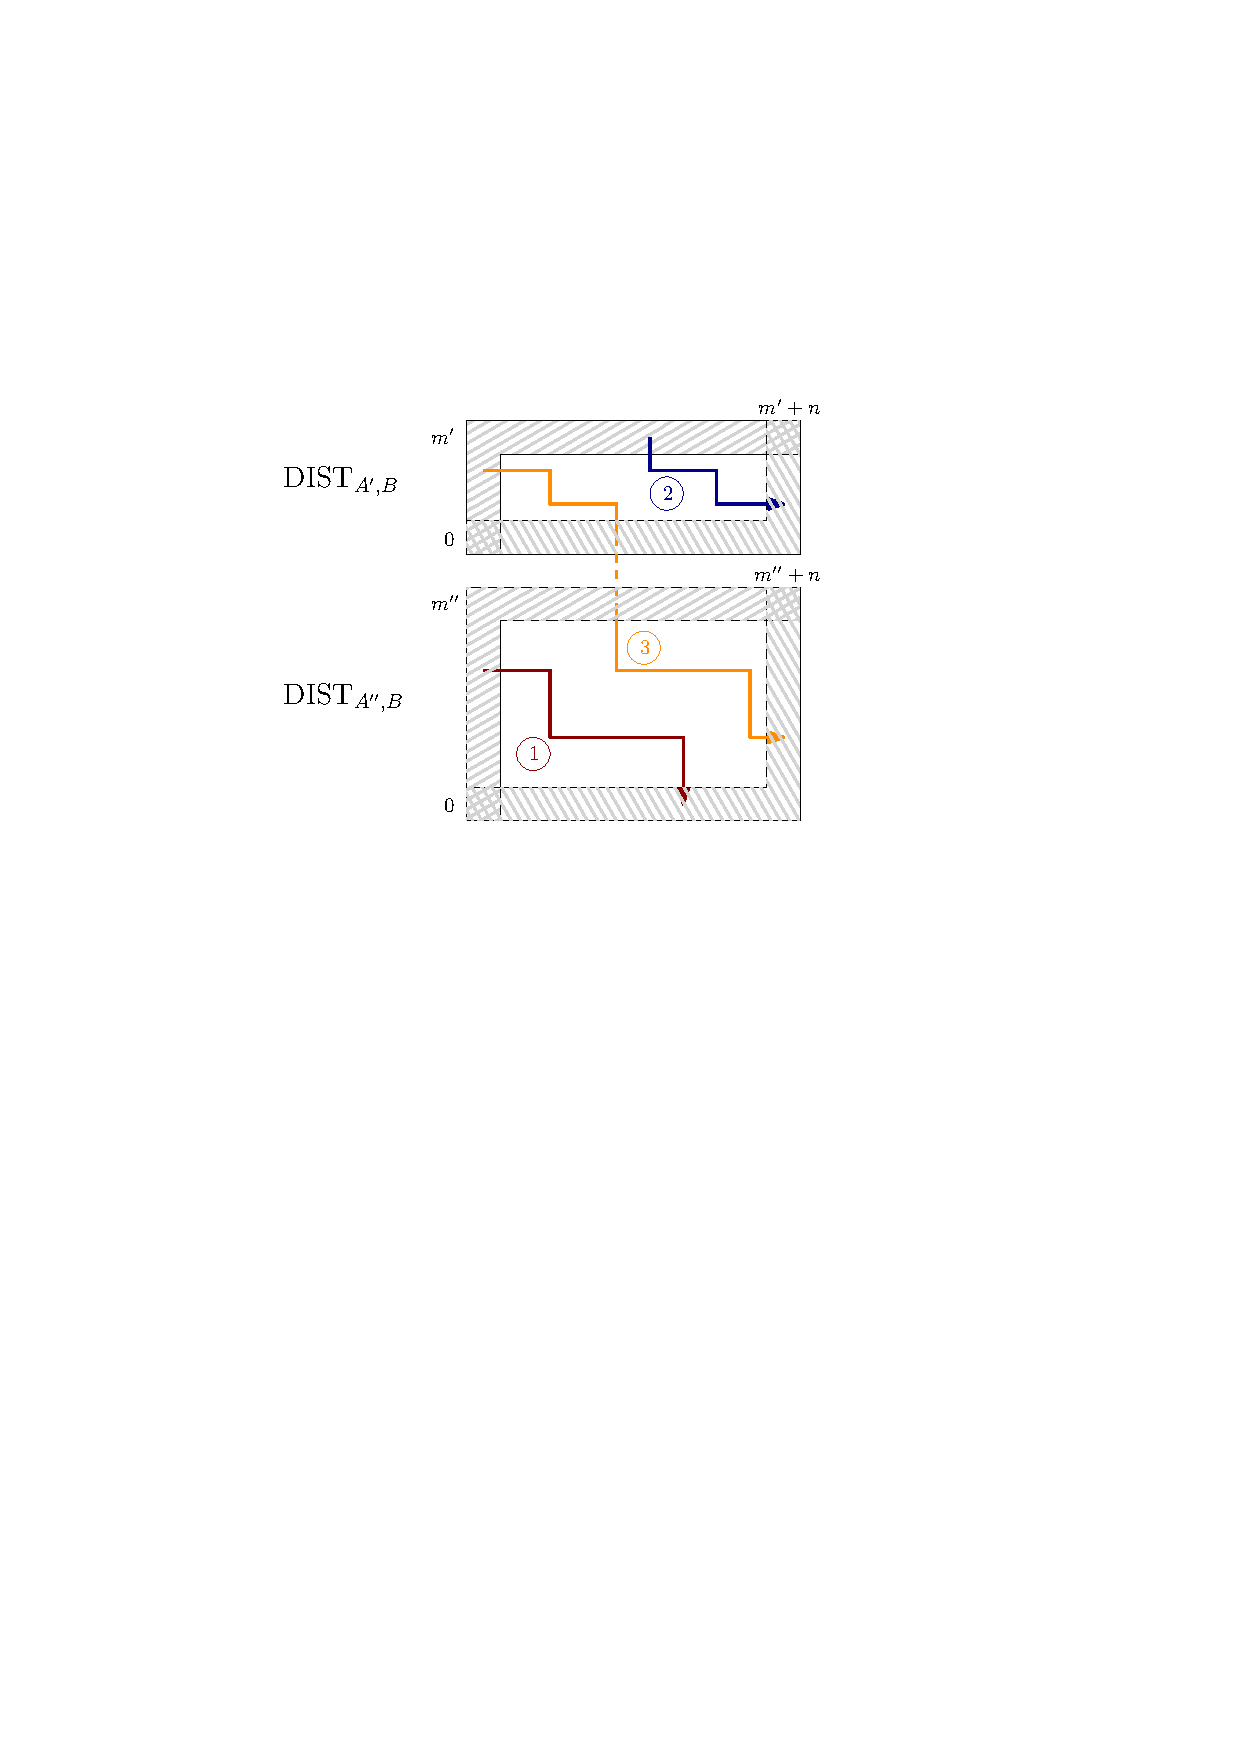
\includegraphics[width=8cm]{images/dist-vertical-merge-cases}
      \caption{The tree possible cases when vertical merging two $\DIST$ tables.}
      \label{fig:dist-vertical-merge-cases}
    \end{figure}
  \end{proof}
\end{claim}
%
The next pages will show that all the three cases can be unified into a single minimum distance product computation. First the result will be derived for case \circled{3} and then it is shown that case \circled{2} and \circled{1} are also handled correctly by the same computation.

First consider case \circled{3}. Using \cref{claim:dist-vertical-merge} the case can be expanded to find that
\begin{align*}
  \DIST_{A'A'',B}[i, j] &= \max_{k \in \{0, \dots, n\} } \left\{ \DIST_{A',B}[i - m'', k] + \DIST_{A'',B}[m'' + k, j] \right\} \\
              &=  \begin{aligned}
                    \max_k \left\{
                      H_{A',B}(i - m'', k) + \left\{
                        \begin{array}{ll}
                          i - m & \text{if } i - m'' < m' \\
                          0     & \text{o/w}
                        \end{array} \right. \right. \\
                      \left. +\,\,H_{A'',B}(m'' + k, j) + \left\{
                        \begin{array}{ll}
                          n - j & \text{if } j \geq n \\
                          0     & \text{o/w}
                        \end{array} \right.
                    \right\}
                 \end{aligned}\\
              &= \max_k \left\{ H_{A',B}(i - m'', k) + H_{A'',B}(m'' + k, j) \right\}
                  \\ &\quad\quad+ \begin{cases}
                      (i - m) + (n - j)   & \text{if } i < m, j \geq n \\
                      i - m               & \text{if } i < m, j < n \\
                      n - j               & \text{if } i \geq m, j \geq n \\
                      0                   & \text{if } i \geq m, j < n
                    \end{cases}.
\end{align*}
Using the relation between $\DIST$ tables and the $H$-table of \cref{lemma:dist-H-relation} it is found that
\begin{align*}
  H_{A'A'',B}(i, j) &= \max_k \left\{ H_{A',B}(i - m'', k) + H_{A'',B}(m'' + k, j) \right\} \\
                    &= \max_k \left\{ k - (i - m'' - m') - P_{A'}^{\Sigma}(i - m'', k) + j - (k + m'' - m'') - P_{A''}^{\Sigma}(k + m'', j) \right\} \\
                    &= j - (i - m) + \max_k \left\{ -\left( P_{A'}^{\Sigma}(i - m'', k) + P_{A''}^{\Sigma}(k + m'', j) \right)  \right\} \\
                    &= j - (i - m) - \min_k \left\{ P_{A'}^{\Sigma}(i - m'', k) + P_{A''}^{\Sigma}(k + m'', j) \right\}.
\end{align*}
This can be used in \cref{lemma:H-permutation-representation} which gives that
\begin{align*}
  P_{A'A''}^{\Sigma}(i, j) &= \min_k \left\{ P_{A'}^{\Sigma}(i - m'', k) + P_{A''}^{\Sigma}(k + m'', j) \right\} \\
                           &= \min_k \{ {IC'_{P_{A'}}}^{\Sigma}(i, k) + {IC''_{P_{A''}}}^{\Sigma}(k, j) \}.
\end{align*}
Therefore the permutation matrix can be found by computing the minimum distance product between the two simple unit-Monge matrices ${IC'_{P_{A'}}}^{\Sigma}$ and ${IC''_{P_{A''}}}^{\Sigma}$. For simple unit-Monge input matrices of size $O(x)$ their minimum distance product can be computed in time $O(x \log{x})$ by an algorithm given by \cite{Tiskin:2010:FDM:1873601.1873704}. The algorithm is described in \cref{sec:algorithm:min-mult-two-unit-monge} of this thesis.

It will now be shown that this computation also gives the result for case \circled{1} where $i \leq m'', j \leq n + m''$. The definition of the $\DIST$ table yields
\begin{align*}
  \DIST_{A'A'',B}[i, j] &= H_{A'A'',B}(i, j) + \left\{
    \begin{array}{ll}
      i - m             & \text{if } j < n \\
      (i - m) + (n - j) & \text{if } j \geq n
    \end{array}
  \right. \\
  &= (i - m) + j - (i - m) - P_{A'A'',B}^\Sigma(i, j) + \left\{
    \begin{array}{ll}
      0             & \text{if } j < n \\
      (n - j)       & \text{if } j \geq n
    \end{array}
  \right. \\
  &= j - P_{A'A'',B}(i, j) + \left\{
    \begin{array}{ll}
      0             & \text{if } j < n \\
      n - j         & \text{if } j \geq n
    \end{array}
  \right. .
\end{align*}
By a similar analysis of the statement given by \cref{claim:dist-vertical-merge}, it is found that
\begin{align*}
  \DIST_{A'A'',B}[i, j] &= \DIST_{A'',B}[i, j] = H_{A'',B}(i, j) + \left\{
    \begin{array}{ll}
      i - m''             & \text{if } j < n \\
      (i - m'') + (n - j) & \text{if } j \geq n
    \end{array}
  \right. \\
  &= j - (i - m'') - P_{A'',B}^{\Sigma}(i, j) + \left\{
      \begin{array}{ll}
        i - m''             & \text{if } j < n \\
        (i - m'') + (n - j) & \text{if } j \geq n
      \end{array} \right. \\
  &= j - P_{A'',B}^{\Sigma}(i, j) + \left\{
    \begin{array}{ll}
      0             & \text{if } j < n \\
      n - j         & \text{if } j \leq n
    \end{array}
  \right. .
\end{align*}
Subtracting the two expressions yields $P_{A'',B}^{\Sigma}(i, j) = P_{A'A'',B}^{\Sigma}(i, j)$. It will now be verified that this is indeed what is begin computed by the minimum distance product from case \circled{3}. Writing from the minimum distance product, it is found that
\begin{align*}
  \circled{$\star$} &= \min_{k \in \{0,\dots,n+m\}} \{ {IC'_{P_{A'}}}^{\Sigma}(i, k) + {IC''_{P_{A''}}}^{\Sigma}(k, j) \} \\
  &= \min\left\{
       \min_{k \in \{0,\dots,i\}}{P_{A'',B}^{\Sigma}(k, j)},
       \min_{k \in \{i + 1, n + m\}}\left\{ k - i + \left\{ % A row <= m'' in IC' is like: 0 ... 0 1 2 3 4 ...
        \begin{array}{ll}
          P_{A'',B}^{\Sigma}(k, j) & \text{if } k \leq n + m'' \\
          0                        & \text{if } k > n + m''
        \end{array}
       \right. \right\}
     \right\}.
\end{align*}
%
In order to simplify the expression the following claim is useful.
%
\begin{claim}
  \label{claim:bounding-sigma}
  The following bound is valid $\forall k \in \mathbb{N}: i + k \leq n + m''$:
  \[
    P_{A''}^{\Sigma}(i, j) \leq k + P_{A''}^{\Sigma}(i + k, j)
  \]
  \begin{proof}
    Follows almost directly from decreasing unit monotonicity of the $\Sigma$-operator used on permutation matrices in both coordinates (only the $i$ coordinate monotonicity is used here).
  \end{proof}
\end{claim}
Using \cref{claim:bounding-sigma} at the boundary condition $i + k = n + m''$, it is found that $P_{A''}^{\Sigma}(i, j) \leq n + m'' - i + P_{A''}^{\Sigma}(n + m'', j) = n + m'' - i$. Hence, by first using decreasing unit monotonicity of the $\Sigma$-operator and \cref{claim:bounding-sigma} followed by the claim at the boundary condition, it follows that
\[
  \circled{$\star$} = \min\{ P_{A''}^{\Sigma}(i, j), \min_{k \in \{n+m'', \dots, n+m\}} \{ k - i \} \}
                    = P_{A''}^{\Sigma}(i, j) .
\]
Therefore, the minimum distance product computed in case \circled{3} also gives the correct result for case \circled{1}.

Case \circled{2} follows by almost the same arguments as case \circled{1}. First \cref{lemma:dist-H-relation} and the definition of the $H$-table is used on \cref{claim:dist-vertical-merge} yielding
\begin{align*}
  \DIST_{A'A'',B}[i, j] &= \DIST_{A',B}[i - m'', j - m''] \\
    &= H_{A',B}(i - m'', j - m'') +
      \begin{cases}
        (i - m'' - m') + (n - (j - m'')) & \text{if } i - m'' < m' \\
        n - (j - m'')                    & \text{if } i - m'' \geq m'
      \end{cases} \\
    &= n + m'' - j + H_{A',B}(i - m'', j - m'') +
      \begin{cases}
        i - m   & \text{if } i < m \\
        0       & \text{o/w}
      \end{cases} \\
    &= n - (i - m) - P_{A',B}^{\Sigma}(i - m'', j - m'') +
      \begin{cases}
        i - m   & \text{if } i < m \\
        0       & \text{o/w}
      \end{cases}
\end{align*}
Similarly writing out directly from the definition, it is found that
\begin{align*}
  \DIST_{A'A'',B}[i, j] &= H_{A'A'',B}(i, j) +
    \begin{cases}
      (i - m) + (n - j) & \text{if } i < m \\
      n - j             & \text{if } i \geq m
    \end{cases} \\
  &= n - (i - m) - P_{A'A'',B}^{\Sigma}(i, j) +
    \begin{cases}
      i - m & \text{if } i < m \\
      0     & \text{if } i \geq m
    \end{cases}
\end{align*}
This implies that $P_{A'A'',B}^{\Sigma}(i, j) = P_{A',B}^{\Sigma}(i - m'', j - m'')$. As will be seen, this is also what is computed by the minimum distance product of case \circled{3}. Writing out the result of the minimum distance product, it is found that
\begin{align*}
  \circled{$\dagger$} &= \min_{k\in \{ 0, \dots, n + m \}} { {IC'_{P_{A'}}}^{\Sigma}(i, k) + {IC''_{P_{A''}}}^{\Sigma}(k, j) } \\
              &=  \begin{aligned} \min
                    &\left\{
                      \min_{k \in \{0, \dots, m''\}} { P_{A'}^{\Sigma}(k, n + m'') + I^{\Sigma}(0, j - (n + m'')) }, \right. \\
                    &\left.
                      \min_{k \in \{m', \dots, n + m''\}} {P_{A'}^{\Sigma}(i - m'', k - m'') + I^{\Sigma}(0, j - (n + m''))}, \right. \\
                    &\left.
                      \min_{k \in \{ n + m'', \dots, n + m \}} {P_{A'}^{\Sigma}(i - m'', k - m'') + I^{\Sigma}(k - (n + m''), j - (n + m''))}
                    \right\}
                  \end{aligned}
\end{align*}
Notice that the second case always dominates the first, hence the second case can safely be removed from the minimization. Furthermore, the third case can be split, giving
\begin{align*}
  \circled{$\dagger$} &=  \begin{aligned} \min
                    &\left\{
                      n + m'' + j - n - m'',
                      \min_{k \in \{n + m'', j\}} {j - k + P_{A'}^{\Sigma}(i - m'', k - m'')}, \right. \\
                    &\left.
                      \min_{k \in \{j, \dots, n + m\}} {P_{A'}^{\Sigma}(i - m'', k - m'')}
                    \right\}
                  \end{aligned} \\
              &= \begin{aligned} \min
                    &\left\{
                      j,\quad
                      \min_{k \in \{j, \dots, n + m\}} {j - k + P_{A'}^{\Sigma}(i - m'', k - m'')},\quad
                      P_{A'}^{\Sigma}(i - m'', j - m'')
                    \right\}
                  \end{aligned}
\end{align*}
The following claim will help to simplify the expression.
\begin{claim}
  \label{claim:bounding-sigma-col}
  The following bound is valid $\forall a \in \{0, \dots, j\}$:
  \[
    P_{A'}^{\Sigma}(i - m'', j) \leq a + P_{A'}^{\Sigma}(i - m'', j - a)
  \]
  \begin{proof}
    Follows from unit monotonicity of the $\Sigma$-operator on permutation matrices.
  \end{proof}
\end{claim}
By applying \cref{claim:bounding-sigma-col} with $a = j - k$, it is found that
\[
  P_{A'}^{\Sigma}(i - m'', j - m'') \leq (j - k) + P_{A'}^{\Sigma}(i - m'', j - m'' - (j - k)) = (j - k) + P_{A'}^{\Sigma}(i - m'', k - m'').
\]
This eliminates the middle case of the minimization in $\circled{$\dagger$}$. Moreover, \cref{claim:bounding-sigma-col} is used to find that
\[
  P_{A'}^{\Sigma}(i - m'', j - m'') \leq (j - m'') + P_{A'}^{\Sigma}(i - m'', 0) = j - m'' \leq j,
\]
which directly gives that $\circled{$\dagger$} = P_{A'}^{\Sigma}(i - m'', j - m'')$. Therefore the minimum distance product can also be used to solve case \circled{2}. The above calculations establish the following important theorem.
\begin{theorem}[\refbook{p.-55}{Theorem 4.19}]
  \label{thm:dist-vertical-merge}
  Given two $\DIST$ tables $DIST_{A',B}$ and $\DIST_{A'',B}$ with representations $P_{A'}$ and $P_{A''}$ they can be merged into $\DIST_{A'A'',B}$ with representation $P_{A'A''}^{\Sigma}$ by setting
  \[
    P_{A'A''} = IC'_{P_{A'}} \boxdot IC''_{P_{A''}} .
  \]
\end{theorem}

 Therefore two $\DIST$ tables can be merged vertically by a single minimum distance product taking $O(x \log{x})$ time using the algorithm described in \cref{sec:algorithm:min-mult-two-unit-monge}.

\subsubsection{Horizontal merge}
The horizontal merge will be carried out by means of a vertical merge. In order to do this, it should be efficient to compute $\DIST_{B,A}$ from $\DIST_{A,B}$. It turns out that this indeed is the case. In order to see this, the following claim provides an insightful result.
\begin{claim}[\refbook{p.-52}{Lemma 4.14, mentioned but not proved}]
  \label{claim:H_string_switch_relation}
  For all $i, j \in \{0, \dots, n + m\}$ the following identity holds
  \[
    H_{A,B}(i, j) = (m - i) - (n - j) + H_{B,A}(n + m - i, n + m - j)
  \]
  \begin{proof}
    The proof is a case analysis of \cref{def:H-table}.
    \begin{description}
      \item[\circled{1}]: For $i \in \{0, \dots, m\}, j \in \{0, \dots, n\}$
        \begin{align*}
          H_{A,B}(i, j) &= (m - i) + lcs(\substr{A}{m - i}{m}, \substr{B}{0}{j}) \\
            &= (m - i) + lcs(\substr{B}{0}{j}, \substr{A}{m - i}{m}) \\
            &= (m - i) - (n - j) + lcs(B, \substr{A}{m - i}{m} ?^{n - j}) \\
            &= (m - i) - (n - j) + lcs(B, \substr{?^nA?^n}{n + m - i}{m + n + n - j}) \\
            &= (m - i) - (n - j) + H_{B,A}(n + m - i, n + m - j)
        \end{align*}

      \item[\circled{2}]: For $i \in \{m, \dots, m+n\}, j \in \{0, \dots, n\}$
        \begin{align*}
          H_{A,B}(i, j) &= lcs(A, \substr{B}{i - m}{j}) = lcs(\substr{B}{i - m}{j}, A) \\
            &= lcs(B, \substr{?^n A ?^n}{n - (i - m)}{n + m + (n - j)}) - (i - m) - (n - j) \\
            &= (m - i) - (n - j) + H_{B,A}(m + n - i, m + n - j)
        \end{align*}

      \item[\circled{3}]: For $i \in \{0, \dots, m\}, j \in \{n, \dots, n+m\}$
        \begin{align*}
          H_{A,B}(i, j) &= (m - i) - (n - j) + lcs(\substr{A}{m - i}{m - (j - n)}, B) \\
            &= (m - i) - (n - j) + lcs(B, \substr{?^n A ?^n}{m + n - i}{m + n - (j - n)}) \\
            &= (m - i) - (n - j) + H_{B,A}(m + n - i, m + n - j)
        \end{align*}

      \item[\circled{4}]: For $i \in \{m, \dots, m+n\}, j \in \{n, \dots, n+m\}$
        \begin{align*}
          H_{A,B}(i, j) &= (j - n+ lcs(\substr{A}{0}{m - (j - n)}, \substr{B}{i - m}{n})) \\
            &= (j - n) + lcs(\substr{B}{i - m}{n}, \substr{A}{0}{m + n - j}) \\
            &= (j - n) + lcs(B, \substr{?^n A ?^n}{n - (i - m)}{n + m + n - j}) - (i - m) \\
            &= (m - i) - (n - j) + H_{B,A}(n + m - i, m + n - j)
        \end{align*}
    \end{description}
  \end{proof}
\end{claim}
%
The observation of the following claim will be useful later.
%
\begin{claim}
  \label{claim:sum_top_described_as_sum_bottom}
  For all $i, j \in \{0, \dots, n + m\}$ it is the case that
  \[
    \sum_{\substack{ \hat{i} \in \{i, \dots, n + m - 1\} \\ \hat{j} \in \{ 0, \dots, j - 1 \}}} P_{B,A}(m + n - \hat{i}, m + n - \hat{j})
      = j - i + P_{B,A}^{\Sigma}(m + n - i, m + n - j)
  \]
  \begin{proof}
    Since $P_{B,A}$ is a permutation matrix, it contains exactly one $1$ in every row/column. Therefore the sum over the top-right area, can be found by taking the sum over the entire matrix and subtract the left and bottom part, and then add the double counted overlap see \cref{fig:sum-top-described-as-sum-bottom}.
    \begin{figure}[!htb]
      \centering
      \includegraphics[width=3.5cm]{images/claim-matrix-division}
      \caption{Illustration of how the entries are counted.}
      \label{fig:sum-top-described-as-sum-bottom}
    \end{figure}

    This gives that
    \begin{align*}
      &\sum_{\substack{ \hat{i} \in \{i, \dots, n + m - 1\} \\ \hat{j} \in \{ 0, \dots, j - 1 \}}} P_{B,A}(m + n - \hat{i}, m + n - \hat{j}) \\
      = &\underbrace{(n + m)}_{\text{Entire matrix}} - \underbrace{(m + n - j)}_{\text{Left}} - \underbrace{((m + n) - (m + n - i))}_{\text{Bottom}} + \underbrace{P_{B,A}^{\Sigma}(m + n - i, m + n - j)}_{\text{Overlap}} \\
      = &j - i + P_{B,A}^{\Sigma}(m + n - i, m + n - j).
    \end{align*}
  \end{proof}
\end{claim}
%
It is now possible to show how the representation of the two $\DIST$ tables $\DIST_{A,B}$ and $\DIST_{B,A}$ relate. The relation is given in the following lemma.
%
\begin{lemma}[\refbook{p.-52}{Lemma 4.14, mentioned but not proved}]
  \label{lemma:swap_strings}
  Assuming $P_{A,B}$ is the permutation matrix encoding $\DIST_{A,B}$. Then the $\DIST$-table $\DIST_{B,A}$ is encoded by the permutation matrix $P_{B,A}$ where
  \[
    P_{B,A}(m + n - i, m + n - j) = P_{A,B}(i, j).
  \]
  Notice that the transformed permutation matrix $P_{B,A}$ can easily be computed in linear time by a sweep over the rows of $P_{A,B}$.
  \begin{proof}
    It is needed to show that the $H$-table corresponding to the permutation matrix $P_{B,A}$ conforms to \cref{claim:H_string_switch_relation}.
    \begin{align*}
      H_{A,B}(i, j) &= j - (i - m) - P_{A,B}^{\Sigma}(i, j) \\
        &= j - (i - m) - \sum_{\substack{ \hat{i} \in \{i,\dots,n+m - 1\} \\ \hat{j} \in \{0, \dots, j - 1\}}} P_{A,B}(\hat{i}, \hat{j}) \\
        &= j - (i - m) - \sum_{\substack{ \hat{i} \in \{i, \dots, n + m - 1\} \\ \hat{j} \in \{ 0, \dots, j - 1 \}}} P_{B,A}(m + n - \hat{i}, m + n - \hat{j}) \\
        &\overset{\text{\cref{claim:sum_top_described_as_sum_bottom}}}{=} j - (i - m) - (j - i + P_{B,A}^{\Sigma}(m + n - i, m + n - j)) \\
        &= m - P_{B,A}^{\Sigma}(m + n - i, m + n - j) \\
        &= m - \left( (n + m - j) - ((n + m - i) - n) - H_{B,A}(n + m - i, n + m - j) \right) \\
        &= (m - i) - (n - j) + H_{B,A}(n + m - i, n + m - j)
    \end{align*}
    This matches the statement of \cref{claim:H_string_switch_relation}, which completes the proof.
  \end{proof}
\end{lemma}
%
Since it is known how to merge two $\DIST$ tables vertically, the following theorem follows.
\begin{theorem}
  \label{thm:dist-horizontal-merge}
  Given two $\DIST$ tables $\DIST_{A,B'}$ and $\DIST_{A,B''}$ of size $O(x)$, they can be merged into $\DIST_{A,B'B''}$ in time $O(x\log{x})$.
  \begin{proof}
    Following \cref{lemma:swap_strings} a horizontal merge can be carried out by first swapping the strings, then performing a vertical merge, and then swapping the strings of the merged $\DIST$ table again. Since swapping the strings runs in time $O(x)$, the total time of a horizontal merge is bounded by the time of the vertical merge. Therefore, the total time of either of the merge routines is bounded by $O(x\log{x})$.
  \end{proof}
\end{theorem}
This completes the description on how to build the $\DIST$ repository within the specified time bounds.

\subsection{Applying a $\DIST$ table}
\label{sec:applying-a-dist-table}
What remains is to show how the $\DIST$ repository can be used to fill the dynamic programming grid efficiently. Assume that the outputs of a block in the grid with input $I$ need to be computed. The outputs are given by \cref{eqn:dist-application} which by \cref{lemma:dist-H-relation} can be re-written as
\begin{align*}
  O[j] &= \max_i \left\{ I[i] + \DIST[i, j] \right\} \\
    &= \max_i \left\{ I[i] + H(i, j) + \left\{
      \begin{array}{ll}
        i - m             & \text{if } i < m, j < n \\
        0                 & \text{if } i \geq m, j < n \\
        (i - m) + (n - j) & \text{if } i < m, j \geq n \\
        n - j             & \text{if } i \geq m, j \geq n
      \end{array}
    \right. \right\} \\
    &= \max_i\left\{ \left( I[i] + \left\{
      \begin{array}{ll}
        i - m     & \text{if } i < m \\
        0         & \text{o/w.}
      \end{array}
    \right. \right) + H(i, j) \right\} + \left\{
      \begin{array}{ll}
        n - j     & \text{if } j \geq n \\
        0         & \text{o/w.}
      \end{array}
    \right. .
\end{align*}
Therefore, the output can be evaluated by computing the maximum distance product of the corresponding $H$ table with a slight perturbation of the input array, followed by an addition for every resulting output. \cite{Gawrychowski:2012:FAC:2422024.2422048} gave a linear time algorithm for computing the maximum distance product of an arbitrary vector with a $H$-table which is described in \cref{sec:algorithm:max-mult-H-table-with-vector}. This gives a linear time algorithm for applying a $\DIST$ table.

\section{Efficient simple unit-Monge distance products}
The two basic building blocks for merging and applying DIST tables are the algorithms for computing the minimum/maximum distance product. They both rely on properties of simple unit-Monge matrices in order to obtain faster computation that otherwise possible.

\subsection{Minimum distance product of two simple unit-Monge matrices}
\label{sec:algorithm:min-mult-two-unit-monge}
This section will describe how the minimum distance product of two simple unit-Monge matrices of size $n$ can be calculated in $O(n\log{n})$ time. The algorithm is the main result of \cite{Tiskin:2010:FDM:1873601.1873704} and the result has also been described in \refbook{p. 28}{Theorem 3.16}. The explanation given in \cite{Tiskin:2010:FDM:1873601.1873704} contains an error (or unexplained step) in the end of the algorithm which is fixed in \refbook{p. 28}{Theorem 3.16}. The overall presentation of this algorithm follows the ones in the literature, but additional details are supplied and indices are changed to match the \texttt{C++} implementation.

It is assumed from now on that the input matrices are given by their permutation matrices $P_A$ and $P_B$ both of size $n$. The result of the algorithm should be a permutation matrix $P_C$ such that $P_A \boxdot P_B = P_C$. The algorithm is a divide and conquer algorithm on the input permutation matrices $P_A$ and $P_B$.

The computation is trivial in the base case $n = 1$ since only one permutation matrix of this size exists. In the actual implementation the base case size was chosen to be $k \geq 1$. The reason for choosing a bigger base case is that the constant involved in the algorithm makes it slower than direct evaluation for small input sizes. In practice it was found that $k \approx 20$ was the best performing configuration (see \cref{sec:min-dist-mult-bc}).

For the recursive step the two input permutation matrices are first divided into four of size $\frac{n}{2}$ and two recursive calls are then performed. More specifically the subproblems are defined as
\begin{align*}
  P_{A,lo} = P_A\left[*, 0 : \frac{n}{2}\right], \quad &P_{B,lo} = P_B\left[0 : \frac{n}{2}, *\right] \\
  P_{A,hi} = P_A\left[*, \frac{n}{2} : n\right], \quad &P_{B,hi} = P_B\left[\frac{n}{2} : n, *\right].
\end{align*}
The subproblems are illustrated on \cref{fig:min-mult:subproblems}.
\begin{figure}[!htb]
  \centering
  \includegraphics[width=7cm]{images/min-dist-subproblems}
  \caption{Graphical illustration of the subproblems of the input matrices $P_A$ and $P_B$. The gray rows / columns illustrates rows / columns containing all $0$'s. These are virtually removed when calling recursively.}
  \label{fig:min-mult:subproblems}
\end{figure}

Notice that all of these sub-problems are rectangular matrices of size $n \times \frac{n}{2}$ or $\frac{n}{2} \times n$. However, half of the rows (or columns) contains all zero entries, and they can therefore be virtually removed by doing an appropriate index mapping when doing recursive calls. The results of the recursive calls are denoted by
\[
  P_{C,lo} = P_{A,lo} \boxdot P_{B,lo}, \quad P_{C,hi} = P_{A,hi} \boxdot P_{B,hi}.
\]
The results from the two recursive calls are of size $\frac{n}{2}$. However, by doing the inverse index remapping from the above step, they can be considered as matrices of size $n$ and they satisfy that $P_{C,lo} + P_{C,hi}$ is a permutation matrix since they come from disjoint ranges. From this point on $P_{C,lo}$ and $P_{C,hi}$ will be considered as matrices of size $n$. Notice that when the $\Sigma$-operator is applied to the sub-problem matrices, all the rows (columns) that contain all zeros in the sub-problem matrix will be identical to the previous row (column) in the $\Sigma$'ed version. Therefore all the sub-problem matrices where $\Sigma$ is applied will be indexed as $n \times \frac{n}{2}$ or $\frac{n}{2} \times n$ matrices as this eases index notation.

In the implementation the index transformation is done by supplying vectors containing the current subset of rows and columns that should be considered for the subproblem. Using these vectors and the original input matrices, it is easy to construct and represent a constant time mapping to and from indices in the sub-problem matrices and the original input matrices in both $O(n)$ time and space. Since the mapping is constant time, it is possible to query the position of the $1$ entry in a row or column in the sub-problem matrices.

In the following calculations, let $i, j \in \{0, \dots, n\}$. First notice that the desired result can be written as
\begin{align*}
  P_C^{\Sigma}(i, j) &= \min_{k \in \{0, \dots n\}} \left( P_A^{\Sigma}(i, k) + P_B^{\Sigma}(k, j) \right) \\
    &= \min\left( \min_{k \in \{0, \dots, \frac{n}{2}\}} {P_A^{\Sigma}(i, k) + P_B^{\Sigma}(k, j)}, \min_{k \in \{\frac{n}{2}, \dots, n\}} {P_A^{\Sigma}(i, k) + P_B^{\Sigma}(k, j)} \right).
\end{align*}
The goal is to reduce the two sums inside the minimization to a constant number of lookups in the two results from the recursive calls. To do this notice that
\begin{align*}
  P_{C,hi}^{\Sigma}(0, j) &= \min_{k \in \{0, \dots, \frac{n}{2}\}} \left( P_{A,hi}^{\Sigma}(0, k) + P_{B,hi}^{\Sigma}(k, j) \right) \\
    &= \min_{k \in \{0, \dots, \frac{n}{2}\}} \left( k + P_{B,hi}^{\Sigma}(k, j) \right) = P_{B,hi}^{\Sigma}(0, j)
  \\ \\
  P_{C,lo}^{\Sigma}(i, n) &= \min_{k \in \{0, \dots, \frac{n}{2}\}} \left( P_{A,lo}^{\Sigma}(i, k) + P_{B,lo}^{\Sigma}(k, n) \right) \\
    &= \min_{k \in \{0, \dots, \frac{n}{2}\}} \left( P_{A,lo}^{\Sigma}(i, k) + \frac{n}{2} - k \right)
    = P_{A,lo}^{\Sigma}(i, \frac{n}{2})
\end{align*}
where the last equality in both statements follows since $P_{B,hi}$ and $P_{A,lo}$ are sub-permutation matrices\footnote{A sub-permutation matrix is a permutation matrix but where some of the $1$ entries may be omitted.} and hence can decrease by at most one every time $k$ is increased. These two observations can be used to find that
\begin{align*}
  \min_{k \in \{0, \dots, \frac{n}{2}\}} \left( P_A^{\Sigma}(i, k) + P_B^{\Sigma}(k, j) \right)
    &= \min_{k \in \{0, \dots, \frac{n}{2}\}} \left( P_{A,lo}^{\Sigma}(i, k) + P_{B,lo}^{\Sigma}(k, j) + P_{B,hi}^{\Sigma}(0, j) \right) \\
    &= P_{C,lo}^{\Sigma}(i, j) + P_{B,hi}^{\Sigma}(0, j)
    = P_{C,lo}^{\Sigma}(i, j) + P_{C,hi}^{\Sigma}(0, j)
  \\ \\
  \min_{k \in \{\frac{n}{2}, \dots, n\}} \left( P_A^{\Sigma}(i, k) + P_B^{\Sigma}(k, j) \right)
    &= \min_{k \in \{0, \dots, \frac{n}{2}\}} \left( P_{A,hi}^{\Sigma}(i, k) + P_{A,lo}^{\Sigma}(i, \frac{n}{2}) + P_{B,hi}^{\Sigma}(k, j) \right) \\
    &= P_{C,hi}^{\Sigma}(i, j) + P_{A,lo}^{\Sigma}(i, \frac{n}{2})
    = P_{C,hi}^{\Sigma}(i, j) + P_{C,lo}^{\Sigma}(i, n),
\end{align*}
which give the following correspondence between the result from the recursive calls and the result of the current call
\[
  P_C^{\Sigma}(i, j) = \min\left( P_{C,lo}^{\Sigma}(i, j) + P_{C,hi}^{\Sigma}(0, j),
                                  P_{C,hi}^{\Sigma}(i, j) + P_{C,lo}^{\Sigma}(i, n)
                            \right).
\]
However, there is not enough time to loop through all combinations of $i,j$ since this would take $O(n^2)$ time. Instead three conditions will be established that gives the positions of the $1$'s in $P_C$. In order to do this, the difference between the two arguments in the minimization is considered. Define:
\begin{align*}
  \delta(i, j) :&= \left( P_{C,lo}^{\Sigma}(i, j) + P_{C,hi}^{\Sigma}(0, j) \right) - \left( P_{C,hi}^{\Sigma}(i, j) + P_{C,lo}^{\Sigma}(i, n) \right) \\
    &= \left( P_{C,hi}^{\Sigma}(0, j) - P_{C,hi}^{\Sigma}(i, j) \right) - \left( P_{C,lo}^{\Sigma}(i, n) - P_{C,lo}^{\Sigma}(i, j) \right) \\
    &= \left( \sum_{\substack{\hat{i} \in \{0, \dots, n - 1\} \\ \hat{j} \in \{0, \dots, j - 1\}}} P_{C,hi}(\hat{i}, \hat{j}) - \sum_{\substack{\hat{i} \in \{i, \dots, n - 1\} \\ \hat{j} \in \{0, \dots, j - 1\}}} P_{C,hi}(\hat{i}, \hat{j}) \right) \\ &\quad\quad- \left( \sum_{\substack{\hat{i} \in \{i, \dots, n - 1\} \\ \hat{j} \in \{0, \dots, n - 1\}}} P_{C,lo}(\hat{i}, \hat{j}) - \sum_{\substack{\hat{i} \in \{i, \dots, n - 1\} \\ \hat{j} \in \{0, \dots, j - 1\}}} P_{C,lo}(\hat{i}, \hat{j}) \right) \\
    &= \sum_{\substack{\hat{i} \in \{0, \dots, i - 1\} \\ \hat{j} \in \{0, \dots, j - 1\}}} P_{C,hi}(\hat{i}, \hat{j}) - \sum_{\substack{\hat{i} \in \{i, \dots, n - 1\} \\ \hat{j} \in \{j, \dots, n - 1\}}} P_{C,lo}(\hat{i}, \hat{j})
\end{align*}
Since $P_{C,lo} + P_{C,hi}$ is a permutation matrix, $\delta$ is unit-monotone increasing in both of its arguments. The sign of $\delta(i, i)$ plays a vital role in determining the position of the $1$'s in $P_C$. The following three exhaustive mutual exclusive cases are considered:
\begin{description}
  \item[$\delta(i + 1, j + 1) \leq 0$]: From the monotonicity of $\delta$ it is known that $\delta(k, l) \leq 0$ for all $k \leq i + 1$ and $j \leq j + 1$. Therefore the definition of the $\delta$-function gives that for all such $k$ and $l$'s it is the case that
  \[
    P_C^{\Sigma}(k, l) = P_{C,lo}^{\Sigma}(k, l) + P_{C,hi}^{\Sigma}(0, l).
  \]
  By using the above identity, \cref{claim:sigma-box-identity} and unfolding definitions it is found that
  \begin{align*}
    P_C(i, j) &= (P_C^{\Sigma})^{\Box}(i, j) = P_C^{\Sigma}(i, j + 1) - P_C^{\Sigma}(i, j) - P_C^{\Sigma}(i + 1, j + 1) + P_C^{\Sigma}(i + 1, j) \\
    &= (P_{C,lo}^{\Sigma}(i, j + 1) + P_{C,hi}^{\Sigma}(0, j + 1)) - (P_{C,lo}^{\Sigma}(i, j) + P_{C,hi}^{\Sigma}(0, j)) \\&\quad\quad - (P_{C,lo}^{\Sigma}(i + 1, j + 1) + P_{C,hi}^{\Sigma}(0, j + 1)) + (P_{C,lo}^{\Sigma}(i + 1, j) + P_{C,hi}^{\Sigma}(0, j)) \\
    &= P_{C,lo}^{\Sigma}(i, j + 1) - P_{C,lo}^{\Sigma}(i, j) - P_{C,lo}^{\Sigma}(i + 1, j + 1) + P_{C,lo}^{\Sigma}(i + 1, j) \\
    &= (P_{C,lo}^{\Sigma})^{\Box}(i, j) = P_{C,lo}(i, j).
  \end{align*}

  \item[$\delta(i, j) \geq 0$]: This case is very similar to the first. By monotonicity of $\delta$ it is known that $\delta(k, l) \geq 0$ for all $k \geq i, l \geq l$. For all such $k$ and $l$'s the definition of $\delta$ now gives that
  \[
    P_C^{\Sigma}(i, j) = P_{C,hi}^{\Sigma}(i, j) + P_{C,lo}^{\Sigma}(i, n).
  \]
  Like before \cref{claim:sigma-box-identity} is used to find that
  \begin{align*}
    P_C(i, j) &= (P_C^{\Sigma})^{\Box}(i, j) = P_C^{\Sigma}(i, j + 1) - P_C^{\Sigma}(i, j) - P_C^{\Sigma}(i + 1, j + 1) + P_C^{\Sigma}(i + 1, j) \\
    &= (P_{C,hi}^{\Sigma}(i, j + 1) + P_{C,lo}^{\Sigma}(i, n)) - (P_{C,hi}^{\Sigma}(i, j) + P_{C,lo}^{\Sigma}(i, n)) \\&\quad\quad - (P_{C,hi}^{\Sigma}(i + 1, j + 1) + P_{C,hi}^{\Sigma}(i + 1, n)) + (P_{C,hi}^{\Sigma}(i + 1, j) + P_{C,lo}^{\Sigma}(i + 1, n)) \\
    &= P_{C,hi}^{\Sigma}(i, j + 1) - P_{C,hi}^{\Sigma}(i, j) - P_{C,hi}^{\Sigma}(i + 1, j + 1) + P_{C,hi}^{\Sigma}(i + 1, j) \\
    &= (P_{C,hi}^{\Sigma})^{\Box}(i, j) = P_{C,hi}(i, j).
  \end{align*}

  \item[$\delta(i + 1, j + 1) > 0, \delta(i, j) < 0$]: By unit monotonicity of $\delta$ it must be the case that
  \[
    \delta(i + 1, j) = \delta(i, j + 1) = 0.
  \]
  From the definition of $\delta$, this implies that
  \begin{align*}
    P_C^{\Sigma}(i, j + 1) &= P_{C,lo}^{\Sigma}(i, j + 1) + P_{C,hi}^{\Sigma}(0, j + 1) = P_{C,hi}^{\Sigma}(i, j + 1) + P_{C,lo}^{\Sigma}(i, n) \\
    P_C^{\Sigma}(i + 1, j) &= P_{C,lo}^{\Sigma}(i + 1, j) + P_{C,hi}^{\Sigma}(0, j) = P_{C,hi}^{\Sigma}(i + 1, j) + P_{C,lo}^{\Sigma}(i + 1, n).
  \end{align*}
  Also the assumptions on $\delta$ gives that
  \begin{align*}
    P_C^\Sigma(i, j) &= P_{C,lo}^{\Sigma}(i, j) + P_{C,hi}^{\Sigma}(0, j) < P_{C,hi}^{\Sigma}(i, j) + P_{C,lo}^{\Sigma}(i, n) \\
    P_C^{\Sigma}(i + 1, j + 1) &= P_{C,hi}^{\Sigma}(i + 1, j + 1) + P_{C,lo}^{\Sigma}(i + 1, n) < P_{C,lo}^{\Sigma}(i + 1, j + 1) + P_{C,hi}(0, j + 1).
  \end{align*}
  Using these facts and \cref{claim:sigma-box-identity} it is found that
  \begin{align*}
    P_C(i, j) &= P_C^{\Sigma}(i, j + 1) - P_C^{\Sigma}(i, j) - P_C^{\Sigma}(i + 1, j + 1) + P_C^{\Sigma}(i + 1, j) \\
    &> (P_{C,lo}^{\Sigma}(i, j + 1) + P_{C,hi}^{\Sigma}(0, j + 1)) - (P_{C,lo}^{\Sigma}(i, j) + P_{C,hi}^{\Sigma}(0, j)) \\&\quad\quad - (P_{C,lo}^{\Sigma}(i + 1, j + 1) + P_{C,hi}(0, j + 1)) + (P_{C,lo}^{\Sigma}(i + 1, j) + P_{C,hi}^{\Sigma}(0, j)) \\
    &= P_{C,lo}^{\Sigma}(i, j + 1) - P_{C,lo}^{\Sigma}(i, j) - P_{C,lo}^{\Sigma}(i + 1, j + 1) + P_{C,lo}^{\Sigma}(i + 1, j) \\
    &= P_{C,lo}(i, j)
  \end{align*}
  Since both $P_{C,lo}$ and $P_C$ by \cref{claim:unit-monge-min-prod-closed} are permutation matrices and the strict equality $P_C(i, j) > P_{C,lo}(i, j)$ is established, it must be the case that $P_C(i, j) = 1$.
\end{description}
Summarizing the above cases, $P_C(i, j)$ should contain a $1$ iff one of the following mutual exclusive conditions is satisfied
\begin{align}
  P_{C,lo}(i, j) = 1 &\text{ and } \delta(i + 1, j + 1) \leq 0 \\
  P_{C,hi}(i, j) = 1 &\text{ and } \delta(i, j) \geq 0 \\
  \delta(i + 1, j + 1) > 0 &\text{ and } \delta(i, j) < 0.
\end{align}
The idea is to make it efficient checking when one of the conditions is satisfied. In order to do this, it is needed to be able to efficiently check if the $\delta$ function contains a number $< 0$ or $> 0$. If for a given $i, j$ this can be done in constant time, all the above $\delta$-constraints can be efficiently checked.

To facilitate this check, the $\delta$ function is viewed as a $n \times n$ matrix. From unit monotonicity the entries $< 0$ must be located in the top left part, and the entries $> 0$ must be in the bottom right path as illustrated by \cref{fig:delta-example}. Basically the idea now is to trace two separating paths, separating the entries $< 0$ and the ones $> 0$ from the rest. The separating path for the entries $< 0$ are called $r_{hi}$ and the other is called $r_{lo}$.

\begin{figure}[!htb]
  \centering
  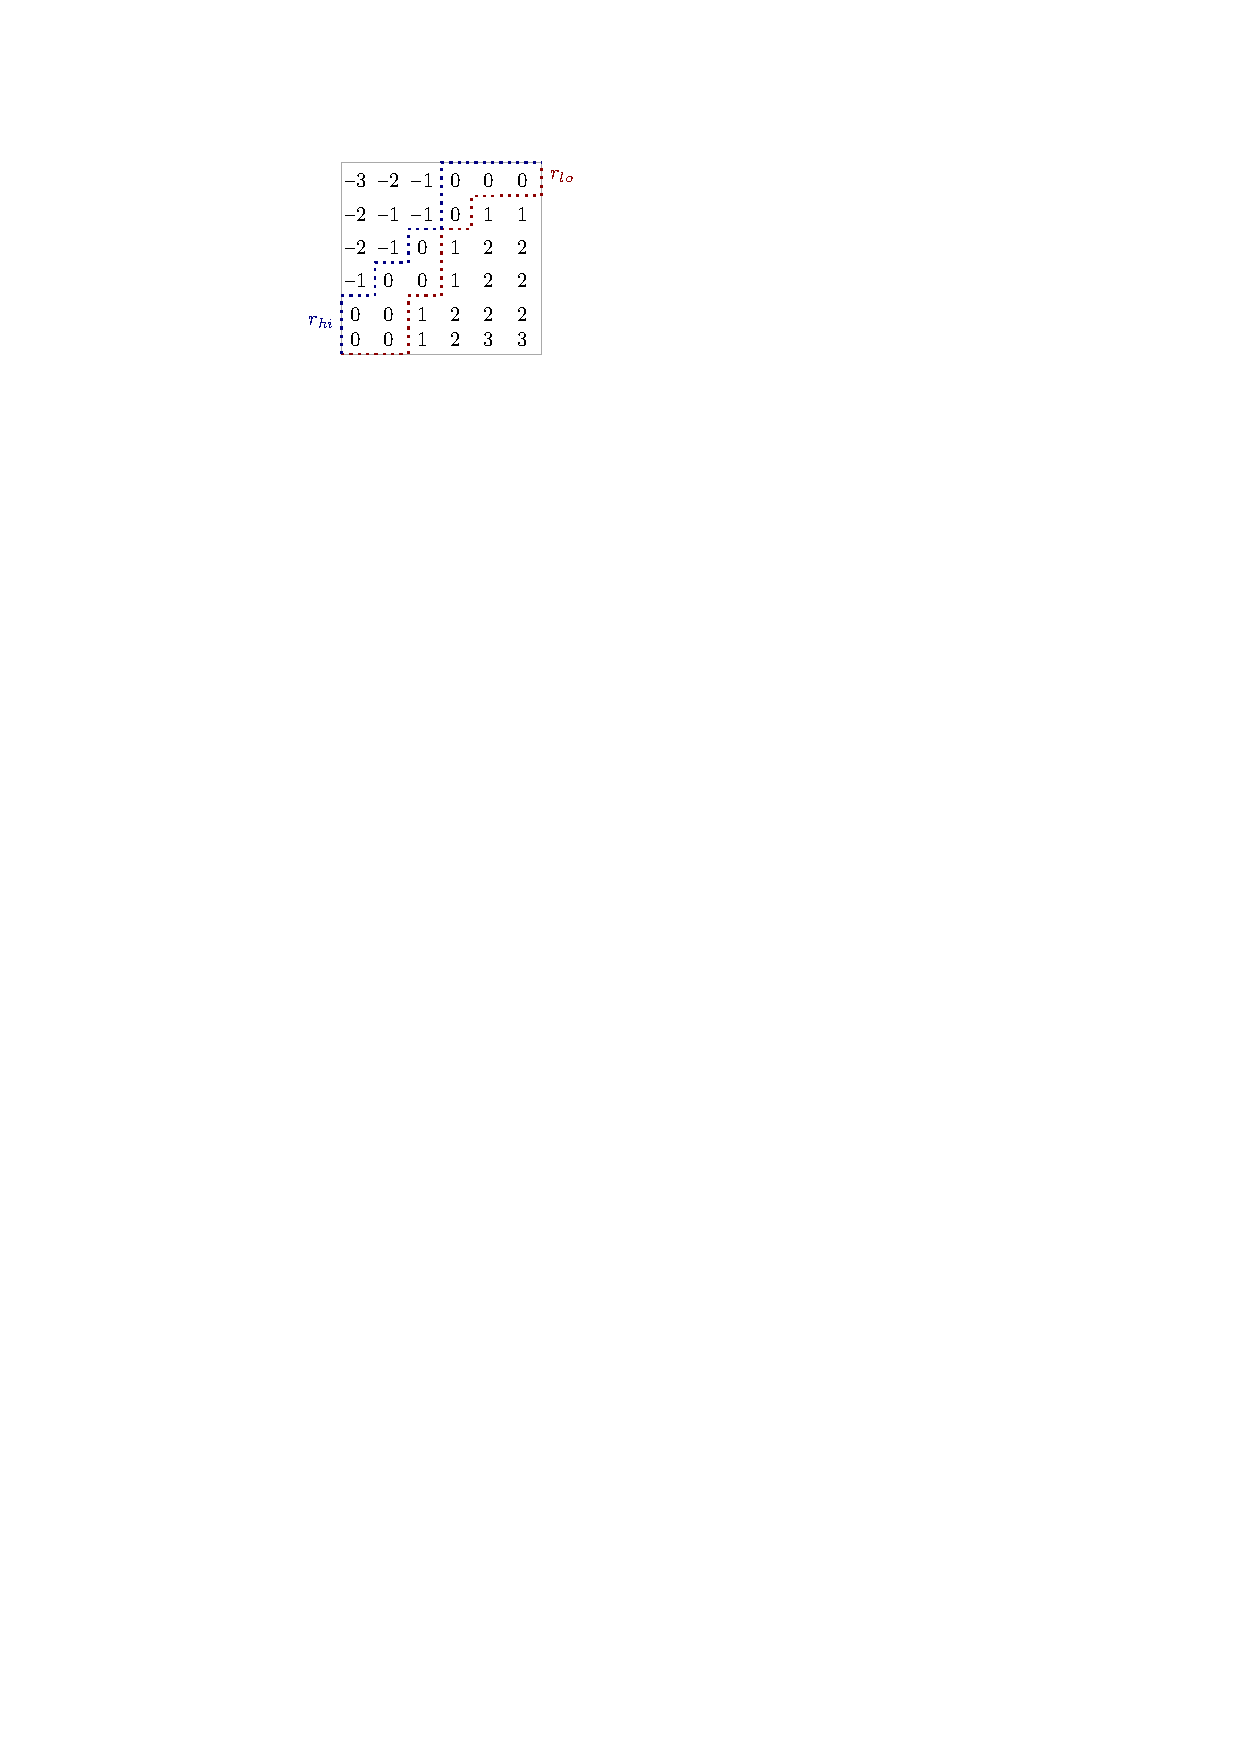
\includegraphics[width=5cm]{images/delta-matrix}
  \caption{Example of the $\delta$-function written as a matrix with separating paths.}
  \label{fig:delta-example}
\end{figure}

Each of these paths is of length exactly $2n$, and the idea is to represent a path, say $r_{hi}$, as an array $r_{hi}$ of length $2n$ such that an entry on the path is given by
\[
  \left( \frac{r_{hi}(d) - d}{2}, \frac{r_{hi}(d) + d}{2} \right)
\]
where $d \in \{-n, \dots, n\}$. That is, if $r_{hi}(-n) := n$, then the starting position becomes $(n, 0)$ which is the desired starting position. Let $d \in \{-n, \dots, n - 1\}$, then if the path should go upward set $r_{hi}(d + 1) = r_{hi}(d) - 1$ because
\begin{align*}
  \frac{r_{hi}(d + 1) - (d + 1)}{2} &= \frac{r_{hi}(d) - 1 - (d + 1)}{2} = \frac{r_{hi}(d) - d}{2} - 1 \quad \text{and} \\
  \frac{r_{hi}(d + 1) + (d + 1)}{2} &= \frac{r_{hi}(d) - 1 + (d + 1)}{2} = \frac{r_{hi}(d) - d}{2}.
\end{align*}
Similarly if the path should go right, then set $r_{hi}(d + 1) = r_{hi}(d) + 1$ since
\begin{align*}
  \frac{r_{hi}(d + 1) - (d + 1)}{2} &= \frac{r_{hi}(d) + 1 - (d + 1)}{2} = \frac{r_{hi}(d) - d}{2} \quad \text{and} \\
  \frac{r_{hi}(d + 1) + (d + 1)}{2} &= \frac{r_{hi}(d) + 1 + (d + 1)}{2} = \frac{r_{hi}(d) - d}{2} + 1.
\end{align*}
Exactly the same encoding is used for the $r_{lo}$ path. In order to actually trace the separating paths, it is required that a $\delta$-entry called the \textit{witness}, adjacent to the current position in the path can be queried in constant time. For the high path, the witness is the entry just above the current position and for the low path it is the one immediately to the right of the current position. In order to compute the witness in constant time, the approach taken in \cref{lemma:simple-unit-monge-query-next} can be almost directly reused as the $\delta$ function is a combination of sums over two permutation matrices.

Since the witness can be computed in constant time, it takes $O(n)$ times to build the two separating paths. Now the $\delta$ checks can be simplified as follows:
\begin{description}
  \item[$\delta(i + 1, j + 1) \leq 0$]: This case happens iff $(i + 1, j + 1)$ is above or on the $r_{lo}$ path. Let $d = (n - (i + 1) + (j + 1)) - n = j - i$ be the number of steps that is required for the path to meet the $(i + 1, j + 1)$ entry. Then $(i + 1, j + 1)$ is above or on $r_{lo}$ iff
  \begin{align*}
         &\frac{r_{lo}(j - i) + j - i}{2} = \frac{r_{lo}(d) + d}{2} \geq j + 1 \\
    \iff &r_{lo}(j - i) + j - i \geq 2(j + 1) \\
    \iff &r_{lo}(j - i) \geq i + j + 2
  \end{align*}

  \item[$\delta(i, j) \geq 0$]: This case happens iff $(i, j)$ is below or on $r_{hi}$. Again define $d = (n - i) + j - n = j - i$ to be the number of steps required to reach entry $(i, j)$. Then $(i, j)$ is below or on $r_{hi}$ iff
  \begin{align*}
         &\frac{r_{hi}(j - i) + j - i}{2} = \frac{r_{hi}(d) + d}{2} \leq j \\
    \iff &r_{hi}(j - i) + j - i \leq 2j \\
    \iff &r_{hi}(j - i) \leq i + j
  \end{align*}

  \item[$\delta(i + 1, j + 1) > 0, \delta(i, j) < 0$]: This happens iff $(i + 1, j + 1)$ is under $r_{lo}$ and $(i, j)$ is above $r_{hi}$. Notice that the number of steps required to reach any of these entries is $d = j - i$. Therefore using the same reasoning as in the previous two cases, the condition is satisfied iff both of the following statements are satisfied
  \begin{itemize}
  \item $r_{lo}(j - i) < j + i + 2$
  \item $r_{hi}(j - i) > j + i$,
  \end{itemize}
  or summarized into a single line iff $r_{lo}(j - i) - 2 < j + i < r_{hi}(j - i)$.
  
  By the unit monotonicity of $\delta$, $r_{lo}$ will be located below $r_{hi}$. For this reason, it will be the case that $r_{lo}(d') \geq r_{hi}(d')$ for all $d' \in \{-n, \dots, n\}$, which squeezes the possible values of $r_{hi}(j - i) \in \{r_{lo}(j - i), r_{lo}(j - i) + 1\}$. However, by construction it must always be the case that $r(d') + d'$ is even, for both $r_{lo}$ and $r_{hi}$. Hence it follows that the condition is satisfied iff $r_{hi}(j - i) = r_{lo}(j - i)$.
\end{description}%
%
The check if $P_C(i, j)$ should contain a $1$ can now be formulated as
\begin{align}
  &P_{C,lo}(i, j) = 1 \text{ and } r_{lo}(j - i) \geq i + j + 2 \\
  &P_{C,hi}(i, j) = 1 \text{ and } r_{hi}(j - i) \leq i + j \\
  &r_{lo}(j - i) = r_{hi}(j - i).
\end{align}
The first two cases can be checked by looping through all the $1$'s in both $P_{C,lo}$ and $P_{C,hi}$ and then for each of them check the corresponding path condition. Each check takes constant time and there are a total of $n$ $1$'s in the two matrices. The $1$'s from the first two cases can thereby be computed in $O(n)$ time.

For the last case, the idea is to loop through all $d \in \{-n, \dots, n\}$ and then check if $r_{lo}(d) = r_{hi}(d)$. If this is the case, then the position corresponding to that path position should be set to $1$. The corresponding path position is by definition given to be
\[
  (i, j) = \left( \frac{r(d) - d}{2}, \frac{r(d) + d}{2} \right).
\]
Therefore the $1$'s from the last case can also be computed in time $O(n)$.

The total time for the algorithm is therefore given by the following recurrence
\begin{align*}
  T(1) &= c \\
  T(n) &= c \cdot n + T\left(\left \lceil \frac{n}{2}\right \rceil \right) + T\left(\left \lfloor \frac{n}{2}\right \rfloor \right) \quad \text{for } n > 1
\end{align*}
for some constant $c \in \mathbb{R}$. This recurrence is well known from ex merge-sort and solves to $O(n \log{n})$.

\subsection{Maximum distance product of $H$-table with vector}
\label{sec:algorithm:max-mult-H-table-with-vector}
In order to apply the DIST tables to fill out the grid, it is required to be able to compute the maximum distance product between an arbitrary vector and a $H$-table. This section will describe the algorithm of \cite[Lemma 2, p. 234]{Gawrychowski:2012:FAC:2422024.2422048} which gives a linear time algorithm for solving the problem.

Let $v$ denote the input vector of size $n$ and assume we are given a $n \times n$ $H$-table $H$. The algorithm incrementally computes the maximum distance product where each iteration takes $O(1)$ time, leading to a $O(n)$ time algorithm. The output of the algorithm should be
\[
  u(j) = \max_i v(i) + H(i, j) = \max_i v(i) + j - (i - m) - P^{\Sigma}(i, j)
\]
where $P$ is the permutation matrix representation of the $H$-table. By defining $v'(i) = v(i) - i$ and $u'(j) = u(j) - j$ the maximization can be simplified to
\[
  u'(j) = \max_i v'(i) - P^{\Sigma}(i, j).
\]
In the implementation it is not necessary to copy the input because the slightly modified input and output vectors can be "simulated" directly from the original input. However, the redefinition makes the description of the algorithm a bit more clear, and makes it follow \cite[Lemma 2, p. 234]{Gawrychowski:2012:FAC:2422024.2422048}.

Define $t_j(i) := v'(i) - P^{\Sigma}(i, j)$. That is, for a fixed $j$ it contains all the entries from where the maximum entry needs to be found. Assume there exist two indices $i < i'$ such that $t_j(i) \leq t_j(i')$, then because $P$ is a permutation matrix and by the definition of the $\Sigma$-operator, there are two possibilities:
\begin{description}
  \item[$P^{\Sigma}(i', j) = P^{\Sigma}(i', j + 1) - 1$]: In this case it follows by the definition of the $\Sigma$-operator and that $P$ is a permutation matrix that $P^{\Sigma}(i, j) = P^{\Sigma}(i, j + 1) - 1$.  This can be used to find that
  \begin{align*}
    &t_{j + 1}(i) = v'(i) - P^{\Sigma}(i, j + 1) = v'(i) - P^{\Sigma}(i, j) - 1
      = t_{j}(i) - 1 \\
      \leq\quad &t_j(i') - 1 = v'(i') - P^{\Sigma}(i', j) - 1
      = v'(i') - (P^{\Sigma}(i', j + 1) - 1) - 1 \\
      &= v'(i') - P^{\Sigma}(i', j + 1) = t_{j + 1}(i').
  \end{align*}

  \item[$P^{\Sigma}(i', j) = P^{\Sigma}(i', j + 1)$]: A similar calculation can be used in this case. First notice that $P^{\Sigma}(i, j) \leq P^{\Sigma}(i, j + 1)$ which follows since $P$ is non-negative. It is found that
  \begin{align*}
    &t_{j + 1}(i) = v'(i) - P^{\Sigma}(i, j + 1) \leq v'(i) - P^{\Sigma}(i, j) = t_{j}(i) \\
      \leq\quad &t_j(i') = v'(i') - P^{\Sigma}(i', j) = v'(i') - P^{\Sigma}(i', j + 1) = t_{j + 1}(i').
  \end{align*}
\end{description}
%
Therefore, once such two indices $i,i'$ are found, it is in all successive iterations not necessary to consider the entry at position $i$ as $i'$ will always be at least as good.

The idea now is to store a list of candidates that can attain the maximum possible values, and then weed out this list by using the above observation. Therefore a list of candidate indices $i_1 < i_2 < \dots < i_l$ is maintained such that $t(i_1) > t(i_2) > \dots > t(i_l)$, where $t$ denotes the $t$-values for the current value of $j$. This also means that the result of a given iteration is always given by $t(i_1)$.

The first such index list is easy to compute by sweeping from right to left and then pick out the sequence of strictly increasing $t$-values.

Notice that by definition of the $\Sigma$-operator, all entries $t(1), \dots, t(k)$ should be decreased by $1$ when increasing $j$, where $k$ is the row number of the $1$ entry in row $j$ in $P$. In order to be able to do this in constant time, the selected candidates of $t$ are represented by their relative difference. A bit more details on this is given in \cite[Lemma 2, p. 234]{Gawrychowski:2012:FAC:2422024.2422048}.

Doing this, a prefix of the entries can be decreased by decreasing the first entry, and then find the leftmost entry $> k$, and increase this difference by $1$. If some difference reaches $0$ it is removed from the list, as this can never again be a candidate from the condition above.

The only thing that remains is to locate the leftmost candidate $> k$. This can be done using what is called an interval union find data structure. Such a data structure is initialized with an interval of length $n$. In the beginning there are $n$ disjoint, contiguous and evenly distributed intervals. The data structure support the operation to merge two adjacent intervals, and to query the last point contained in some interval.

The interval union find data structure is used as follows: In the beginning all the entries in the $t$-array have their own interval. As more and more candidates are removed from the list, their intervals are joined. Finding the leftmost candidate $> k$ can then be done by issuing a single interval union find query, taking $O(1)$ time \cite{Itai06lineartime}.

\subsubsection{Note on Interval Union Find}
\label{sec:algorithm:interval-union-find}
The interval union find data-structure implemented is the one of \cite{Itai06lineartime}. The algorithm works by blocking the interval into blocks fitting a machine word of size $\Theta(\log{n})$. Operations inside such a block can be supported very efficiently using simple bit operations. Operations spanning blocks are carried out by using an ordinary union find data structure. \cite{Itai06lineartime} shows that this leads to a data-structure using amortized constant time operations.

 Note however that the amortized constant time relies on blocking the input into blocks of size $\Theta(\log{n})$. In the actual implementation, it has been chosen to always use block sizes of machine word $64$ bits, which is a constant. This choice will always perform superior in practice due to practical limit on the input size, but the theoretical running time of the algorithm becomes that of the ordinary union find data structure, which is the inverse Ackermann function. However, for all practical purposes this is also is a constant. Therefore it is not to be expected that the choice of the constant block size will result in weird looking results in the graphs in the following benchmarks.

\clearpage
\section{Benchmarks}
\label{sec:algorithm:benchmarks}
This section will benchmark the compression based edit distance algorithm. Both with respect to the theoretical running time and also by comparing it to the performance of the simple algorithm. First it will be verified that the distance product algorithms performs as expected and then the combined algorithm for computing the edit distance of compressed strings will be evaluated.

\subsection{Distance products}
In this section the distance product operations on unit-Monge matrices will be benchmarked and optimized for later use.

\subsubsection{Minimum distance product}
\label{sec:min-dist-mult-bc}
In order to get the best possible performance for the minimum distance product computation, the size of the base case of the algorithm described in \cref{sec:algorithm:min-mult-two-unit-monge} should be determined. Notice that when benchmarking the algorithm, the same amount of work should be done no matter the input. Therefore the running time should not depend on the content of the input, but only on its size. Therefore, all the benchmarks of the minimum distance product algorithms have been performed with permutation matrices sampled from a uniformly random distribution over all possible permutation matrices of size $n$.

\Cref{fig:benchmark:min-distance:bc} plots the running time normalized by $n\log{n}$ of the algorithm when varying the base case size. The general form of the plot is as expected: A small base case size leads to a larger running time, and a too large base case size will also yield a larger running time. The best compromise seems to be around base case size $k \approx 20$. For all the following measurements in this report a base case size of $k = 20$ has been used.

Another thing to notice about \cref{fig:benchmark:min-distance:bc} is that it looks like, for a fixed base case size, that the normalized running time converges to a constant. This suggests that the theoretical running time is satisfied in practice.

\begin{figure}[h!]
  \centering
  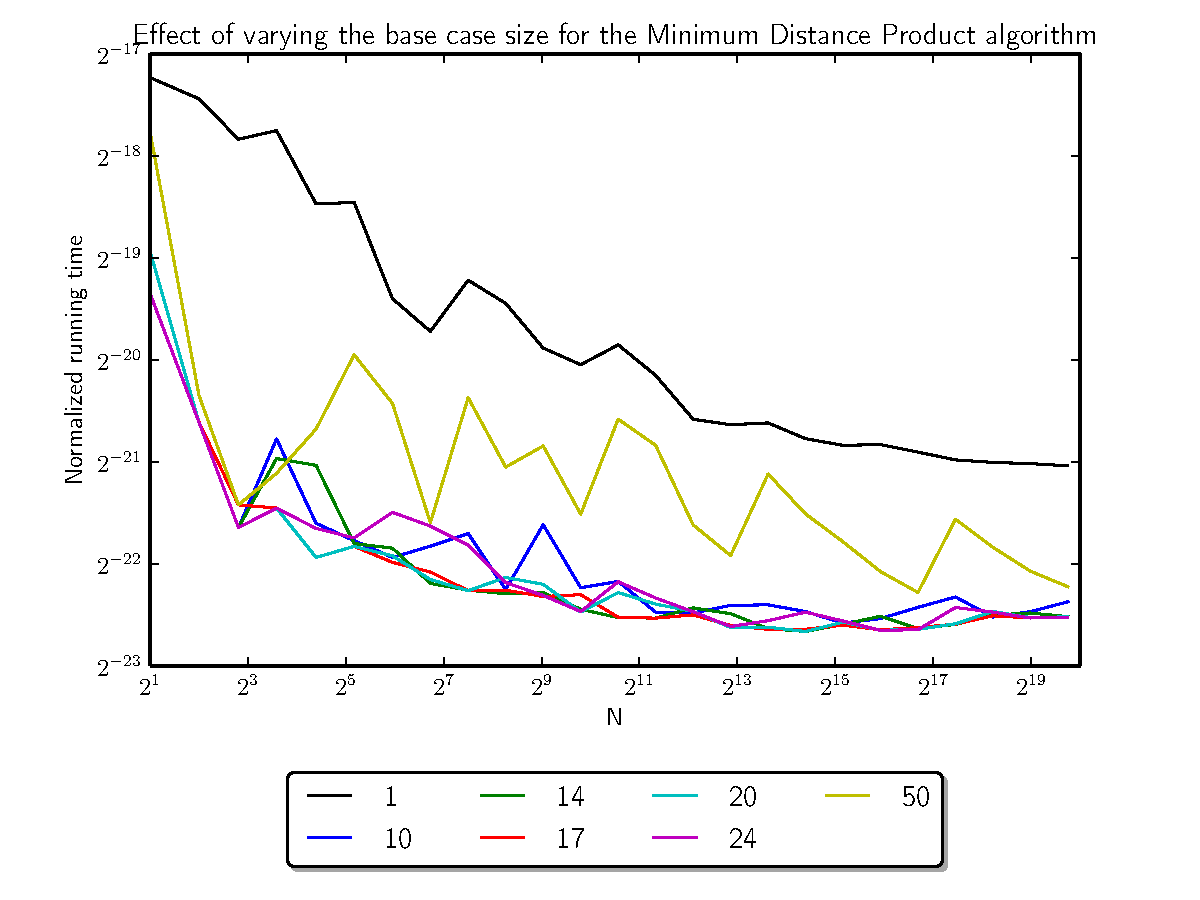
\includegraphics[width=10cm]{distance-mult/min-dist-mult-bc}
  \caption{Normalized running time of the minimum distance product algorithm for varying base case sizes.}
  \label{fig:benchmark:min-distance:bc}
\end{figure}

Notice that the normalized running times for the base case size of $50$ experience periodic peaks. These are due to the actual base case size when running the algorithm. In every step the algorithm splits the input size by $2$ until the input size gets smaller than the base case size. Therefore assuming that the input size is always divisible by $2$, the number of times the input is split becomes $x = \lceil \log{\frac{N}{k}} \rceil$ where $k$ is the base case size. That is, the actual instance size when the base case is hit becomes $\frac{N}{2^x}$. As can be seen on \cref{fig:benchmark:min-distance:bc50} this correlates very nicely with the running time of the algorithm. The reason these jumps are not seen for smaller base case sizes is that the simple unfolding approach is fast for small base case sizes.

\begin{figure}[h!]
  \centering
  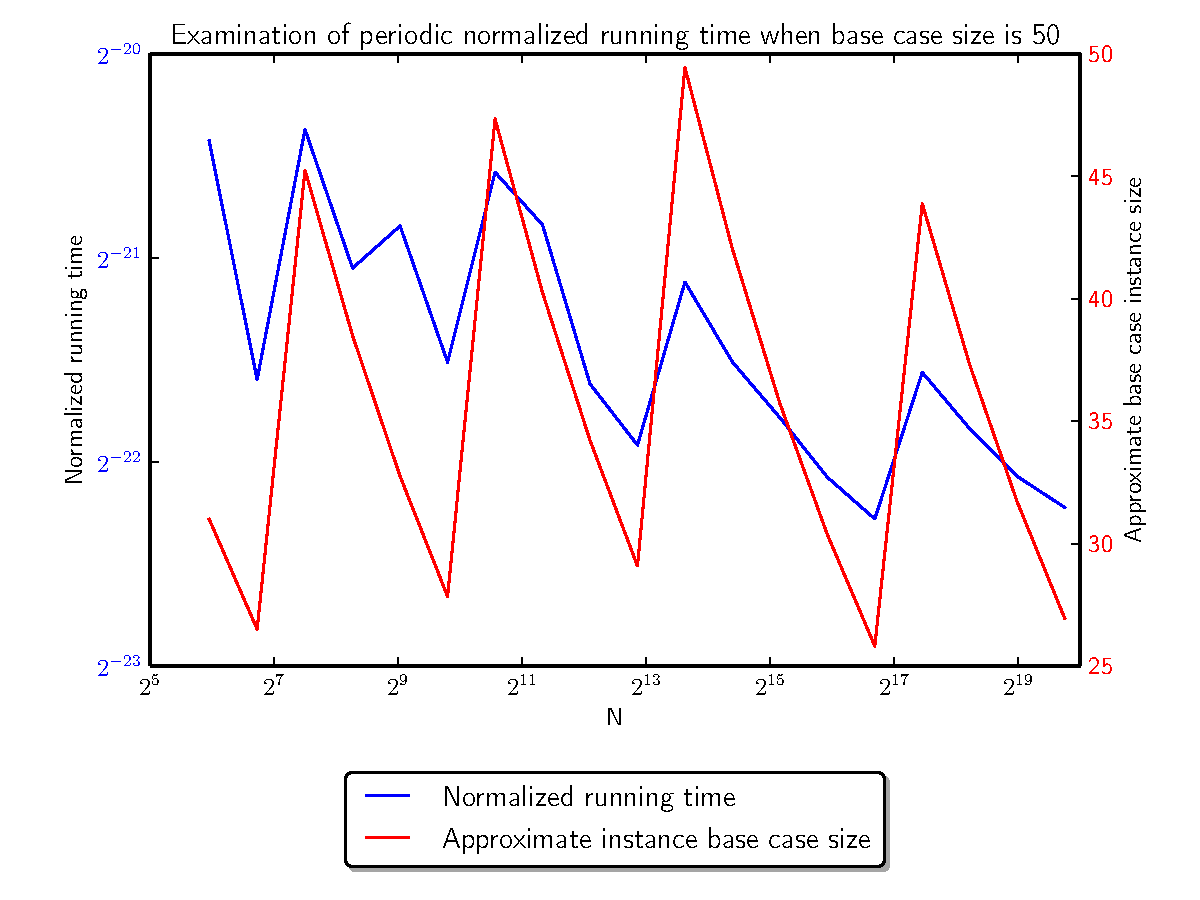
\includegraphics[width=10cm]{distance-mult/min-dist-mult-bc50}
  \caption{Examination of the jumps occurring when the base case size is 50.}
  \label{fig:benchmark:min-distance:bc50}
\end{figure}

\clearpage
\subsubsection{Maximum distance product}
This section will examine if the maximum distance product algorithm runs within the theoretical running time. Also, its running time will be compared to a naive $O(n^2)$ time unfolding algorithm.

The efficient maximum distance product algorithm is a bit more input sensitive than the one for computing the minimum distance product, since a candidate list of possible solutions is maintained. The length of this list does have an influence on the running time. It has been chosen to verify the running time using a permutation matrix sampled uniformly at random. This choice should not have any significant influence on the running time, since the permutation matrix does not directly control the length of the candidate list. For the input vector, three different inputs have been benchmarked:
\begin{description}
  \item[Increasing input] is given by $v_i = i$ for all entries $i$. This type of input should make the candidate list to only be of length 1.
  \item[Decreasing input] is given by the input vector $v_i = 2 \cdot (n - i)$ where $n$ is the input size. This type should make the length of the candidate list as long as possible.
  \item[Random permutation] is a vector $v = \sigma(1, \dots, n)$ where $\sigma \in S_n$. Ie. $v$ is a random permutation of the values $1, \dots, n$.
\end{description}
\Cref{fig:benchmark:max-distance} plots the normalized running time of both the naive $O(n^2)$ algorithm, and the efficient $O(n)$ algorithm of \cite{Gawrychowski:2012:FAC:2422024.2422048}. It can be seen that the algorithm of \cite{Gawrychowski:2012:FAC:2422024.2422048} is superior to the naive algorithm even for relatively small input sizes.

Also, it can be seen that the algorithm behaves as expected wrt. to the different types of input. The input generating the longest candidate list takes the longest time and the one with only one candidate is the fastest.

It can also be seen that the normalized running times seems to be bounded by a constant, which indicates that the theoretical running time is satisfied. However, for large input sizes a small increase in normalized running time for the long candidate list input. From \cref{fig:benchmark:max-distance-cpu} it can be seen that the normalized CPU instructions remain constant as the input size grows. Therefore the increase in running time can be explained by a mismatch with the RAM model and the actual realization of a computer. The measurements from the experiments suggest that the blame is not cache misses as they also approaches a constant when normalized. Therefore it is not exactly known which part of the CPU is responsible for the slight increase in running time, but reasonable guesses could be TLB misses or branch mispredictions.

\begin{figure}[h!]
  \centering
  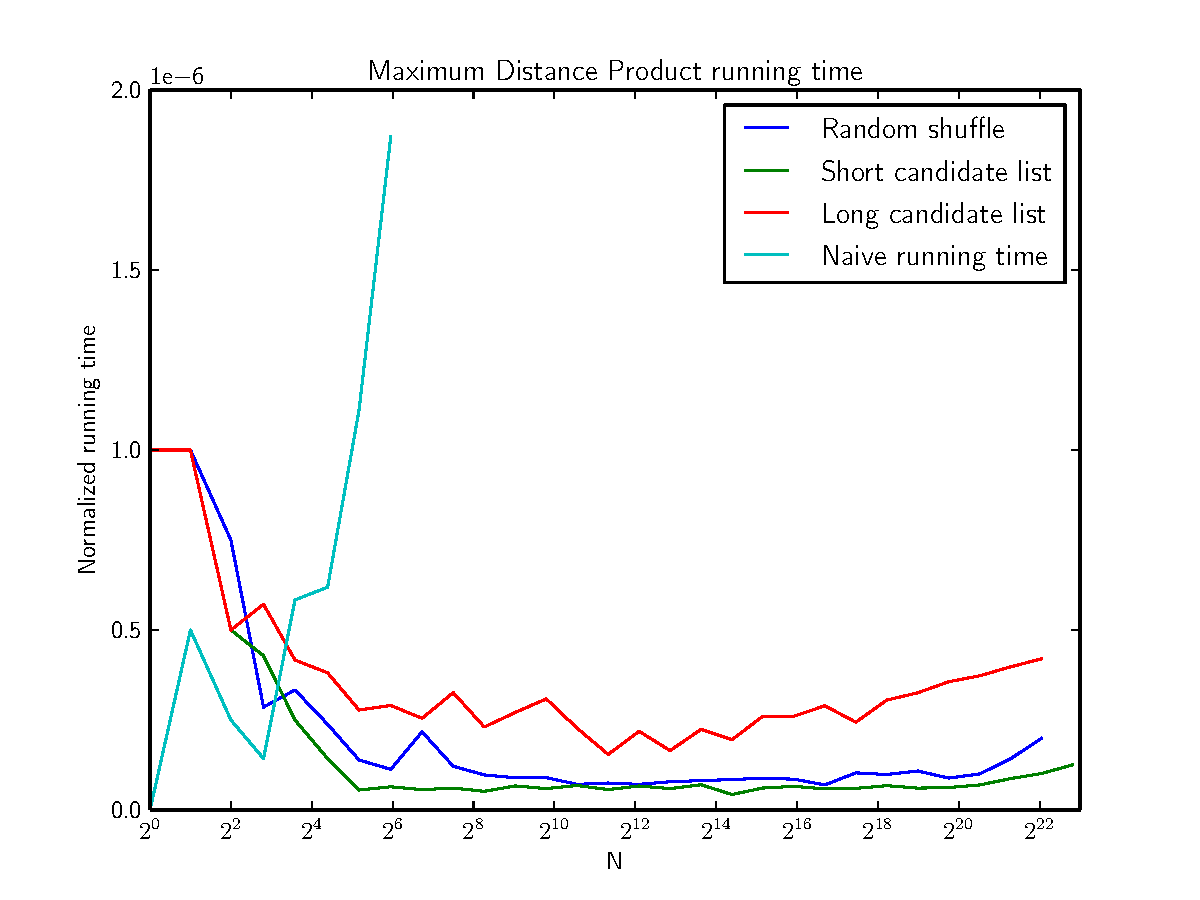
\includegraphics[width=10cm]{distance-mult/max-dist-mult}
  \caption{Running time of the efficient and naive algorithms for computing the maximum distance product of a permutation matrix and a vector.}
  \label{fig:benchmark:max-distance}
\end{figure}

\begin{figure}[!htb]
  \centering
  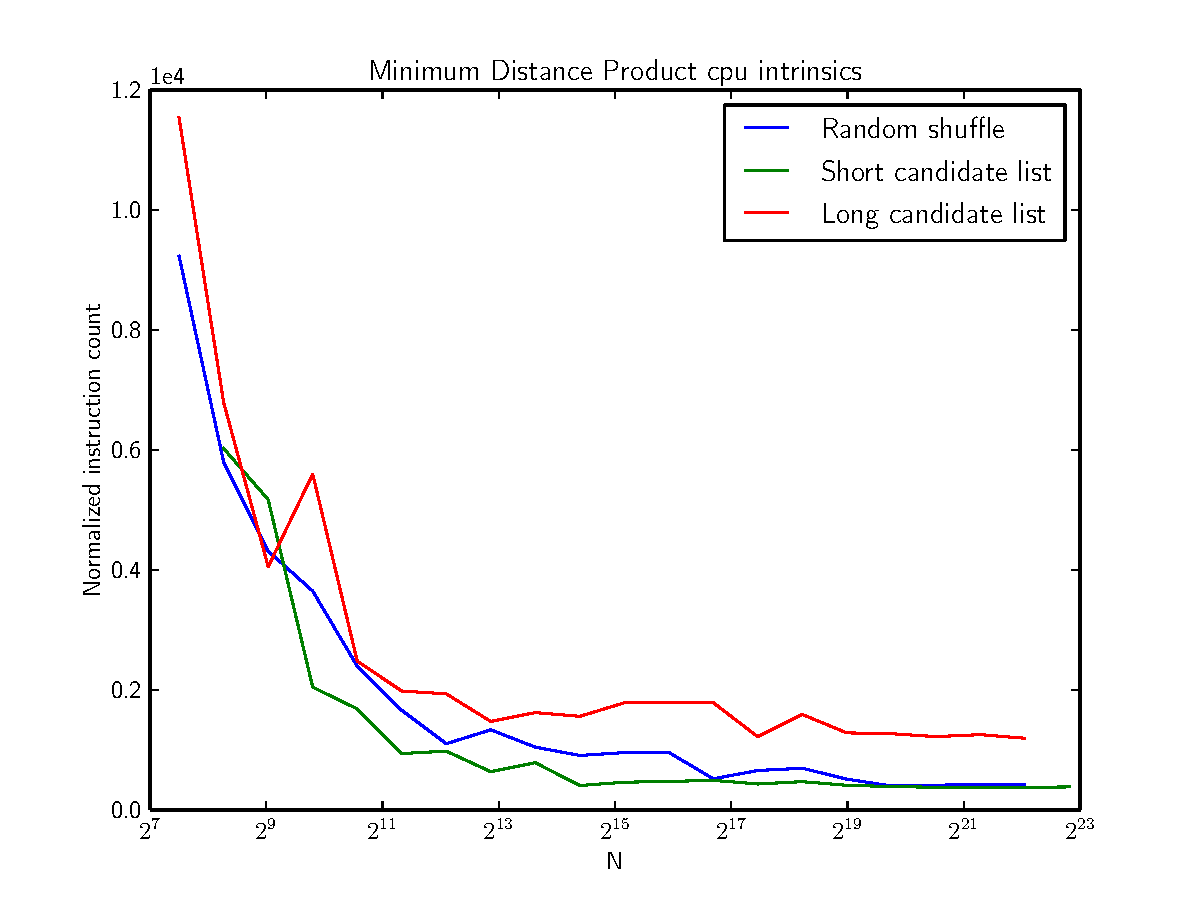
\includegraphics[width=10cm]{distance-mult/max-dist-mult-cpu}
  \caption{Normalized instruction count for the Maximum Distance Multiplication benchmarks.}
  \label{fig:benchmark:max-distance-cpu}
\end{figure}

\clearpage
\subsection{Combined algorithm}
This section will present and discuss measurements of the combined algorithm. First it will be examined that the two main steps of the algorithm (the DIST repository construction and grid computation) satisfies their theoretical running times. Also the time distribution between these two steps will be examined.

In the end it will be checked that all the steps combined into the complete algorithm satisfies the theoretical running time and the running time will be compared to the running time of the simple algorithm on the same inputs.

\subsubsection{Determining SLP partitioning factors}
\label{sec:benchmark:slp-partition-factors}
In \cref{sec:combining-the-two-steps} two factors called $\ffactor$ and $\xfactor$ were introduced. These factors control how large the partitions of the SLPs should be. In this section these factors will be experimentally determined for use in all following benchmarks.

The compressibility of the input may have a big influence on how the factors are optimally chosen. In order to determine what factors to use, an experiment varying the factors while measuring the running time of aligning two Fibonacci strings of length 610 and two random strings of length 610 was performed. The choice of these two input types is due to their very different compression characteristics.

\begin{figure}[!htb]
  \centering
  \begin{subfigure}{0.6\textwidth}
    \centering
    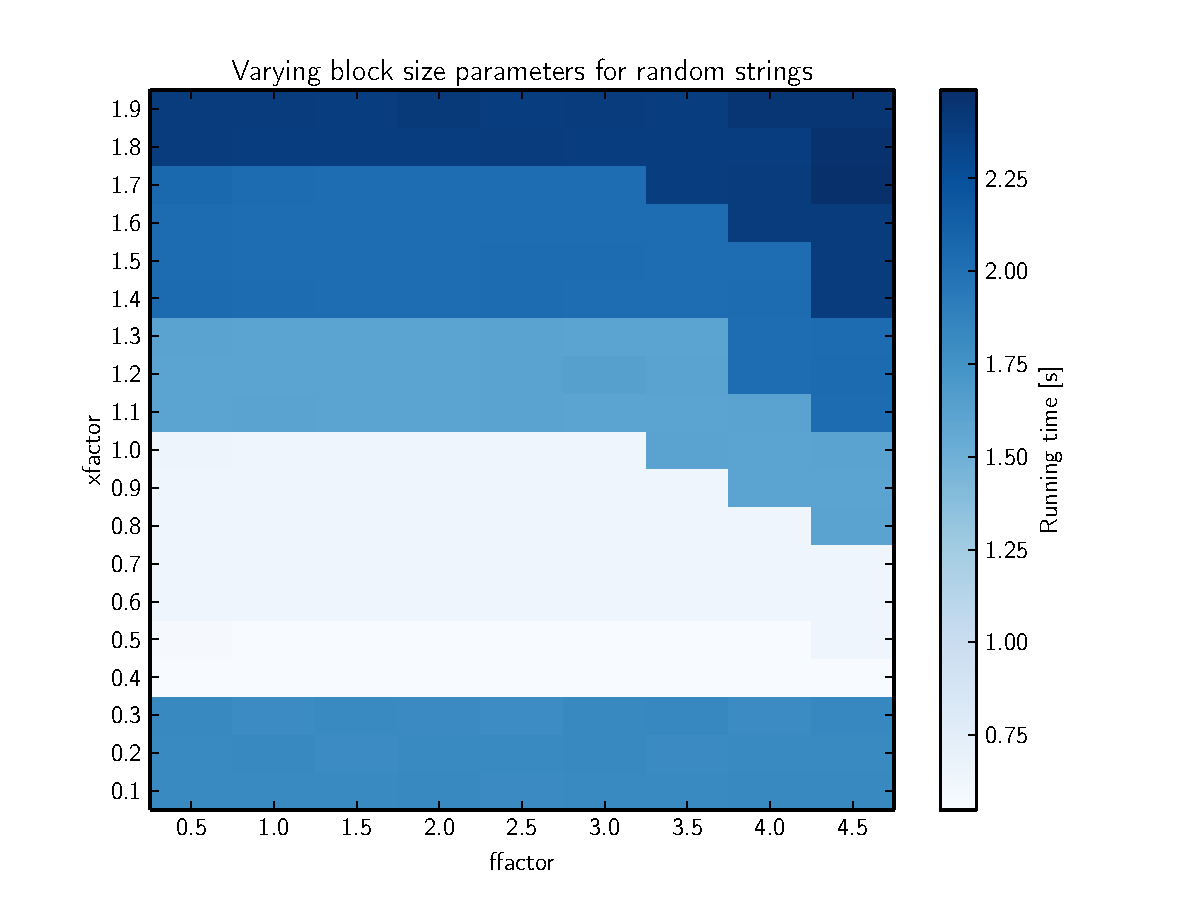
\includegraphics[width=\textwidth]{parameter-test-random}
    \caption{Aligning two Random strings of length 610.}
    \label{fig:benchmark:estimating-factors:random}
  \end{subfigure}\\
  \begin{subfigure}{0.6\textwidth}
    \centering
    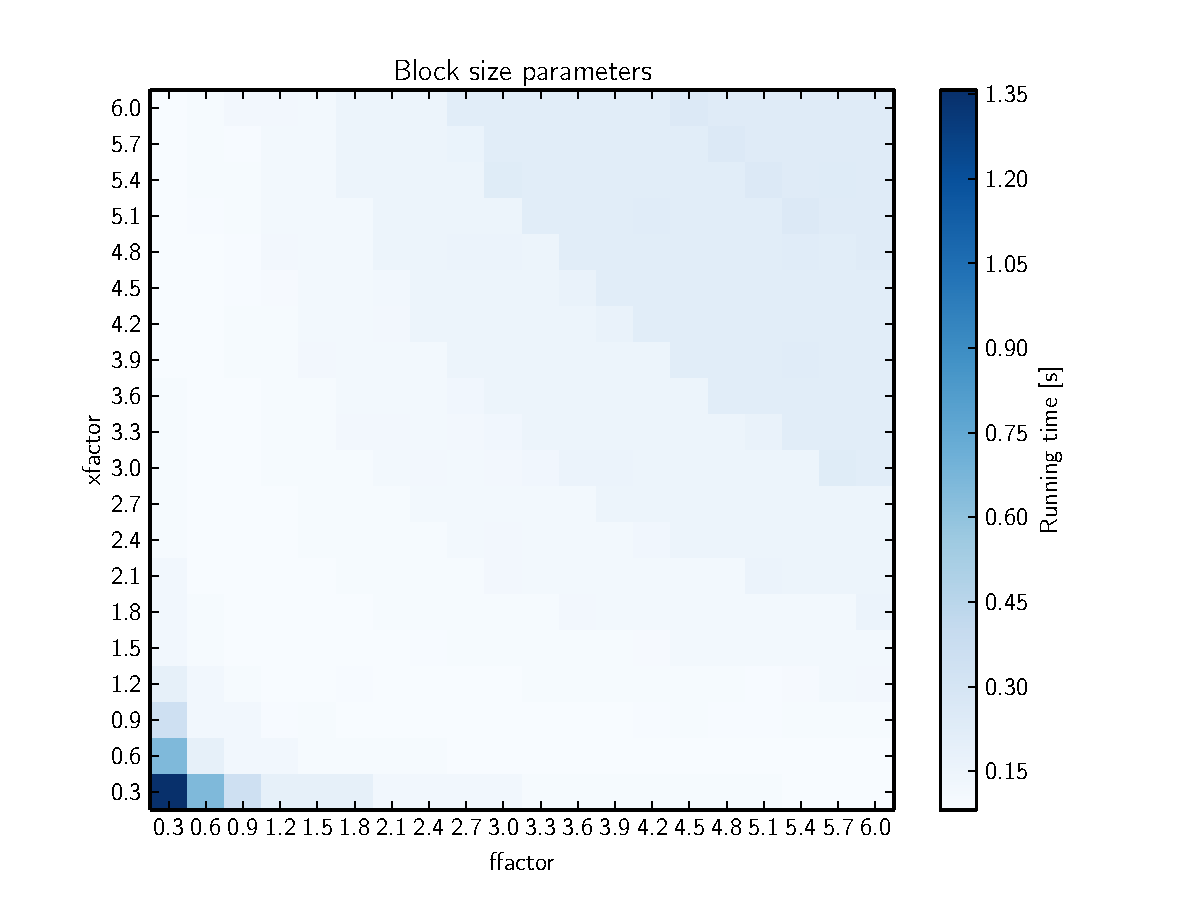
\includegraphics[width=\textwidth]{parameter-test-fib}
    \caption{Aligning two Fibonacci string of length 610.}
    \label{fig:benchmark:estimating-factors:fib}
  \end{subfigure}
  \caption{Plots showing the running time of the edit distance computation when varying $\ffactor$ and $\xfactor$.}
  \label{fig:benchmark:estimating-factors}
\end{figure}

It can be seen on \cref{fig:benchmark:estimating-factors} that the effect of different factors are behaving differently for different input types. This shows that the theoretically choice from \cref{sec:combining-the-two-steps} is a simplification of the real world. In practice the best thing to do is to have a more advanced procedure determining the factors for the given input strings.

\Cref{fig:benchmark:estimating-factors:random} shows that the factors minimizing the running time was $\xfactor = 0.4$ and $\ffactor = 2$. For the following benchmarks this choice will be used for both the random string and the human genome test cases. The reason for choosing the same factors for the human genome is because the compression characteristics of the human genome and a random string was found to be similar in \cref{sec:compression:benchmarks}.

For the Fibonacci string \cref{fig:benchmark:estimating-factors:fib} shows that the best running time is obtained by choosing $\xfactor = 2$ and $\ffactor = 2$. Therefore this choice is used in the following benchmarks for Fibonacci strings.

\clearpage
\subsubsection{DIST Repository and grid computation}
This section will present measurements on the two main steps of the algorithm. Namely construction of the DIST repository and the grid computation.

\paragraph{DIST repository}
First the time taken to build the $\DIST$ repository will be examined. \Cref{fig:benchmark:dist-repo-time} shows the normalized running time for the different input types.
% For the Fibonacci input the normalized running time clearly seems to be bounded by a constant.

% The increase in the normalized running time seen for the random input and human genome for building the DIST repository in the interval $[2^3,2^11]$ can be contributed to a large number of L2 cache misses. \Cref{fig:benchmark:dist-repo-cpu} plots the normalized number of instructions, which in the RAM should be directly correlated to the running time. The normalized instructions converges very quickly towards a constant, meaning that the number of retired instructions are as expected wrt. the theoretical running time. \Cref{fig:benchmark:dist-repo-cpu} also plots the L2 cache miss percentage and it can be seen that the percentage of L2 cache misses is high when the running time of the algorithm increases more than expected. Therefore the increase in wall time can be explained by the hierarchical memory layout of a modern computer.

The normalized runnign time seems to be bounded by a constant for all different types of input. In fact, up to a length of $\approx 2^{13}$ the running time for the random and human genome seems to be decreasing. The same is seen for the Fibonacci string, however its decrease seems to continue throughout all measurements.
Therefore it is concluded that the theoretical running time is satisfied.

\begin{figure}[!htb]
  \centering
  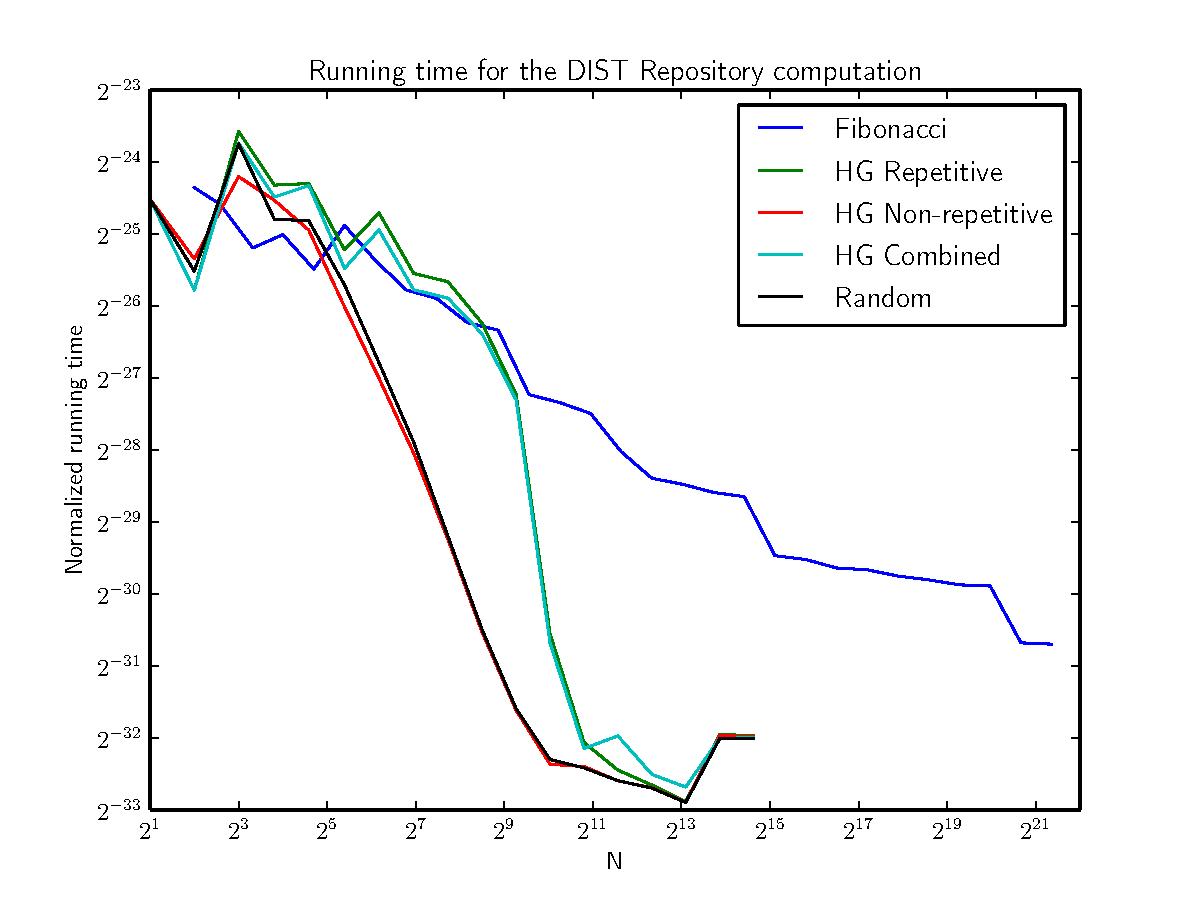
\includegraphics[width=10cm]{combined/dist_runningtime}
  \caption{Plot of the normalized running time for building the DIST repository.}
  \label{fig:benchmark:dist-repo-time}
\end{figure}

% \begin{figure}[!htb]
%   \centering
%   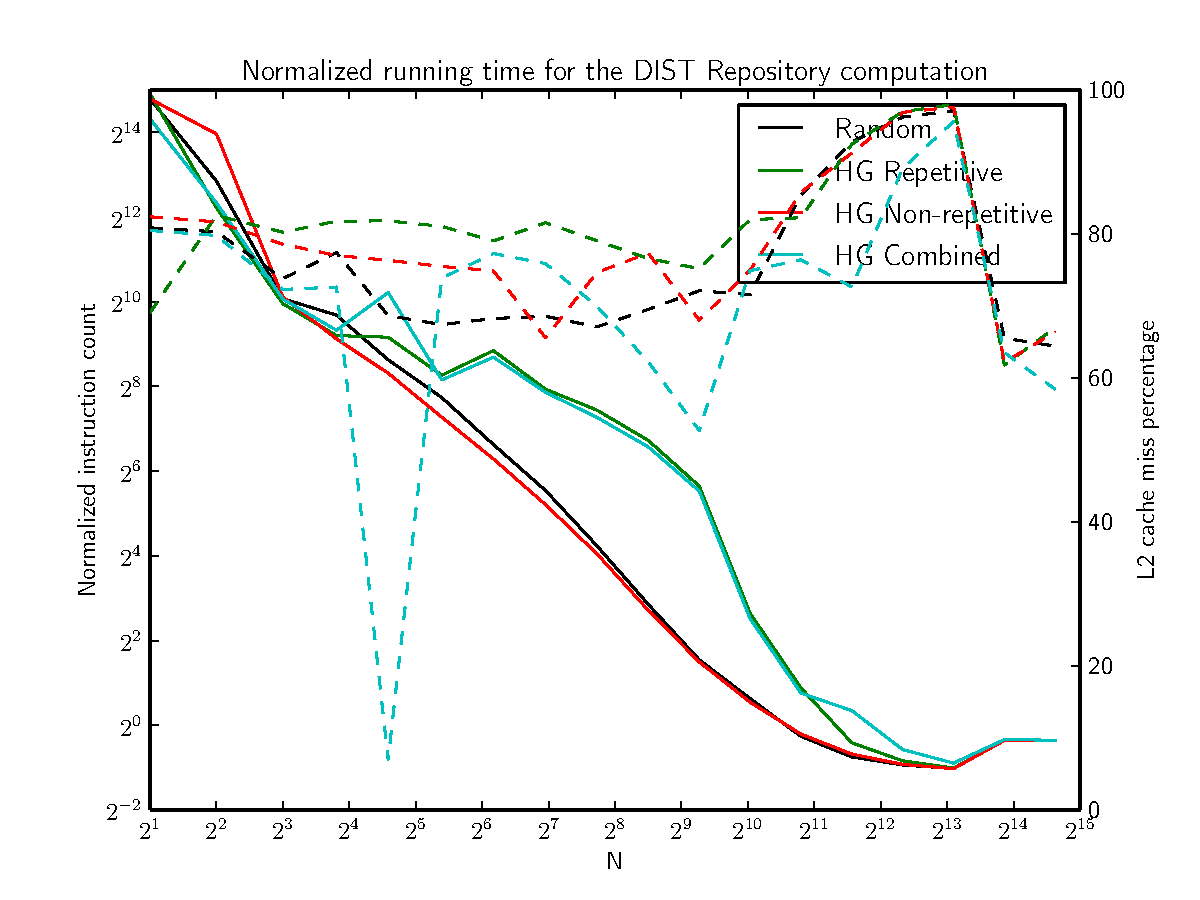
\includegraphics[width=10cm]{combined/dist_runningtime_cpu}
%   \caption{Normalized number of retired instructions and percentage of L2 cache misses when building the DIST repository. The instructions are solid lines and the L2 cache miss percentage are dashed.}
%   \label{fig:benchmark:dist-repo-cpu}
% \end{figure}

\paragraph{Grid computation}
It will now be checked if the time to fill out the dynamical programming grid satisfies the theoretical running time. \Cref{fig:benchmark:fill-grid-time} plots the normalized running time for the different types of input. It can be seen that all the normalized running times seem to be bounded by a constant.
% \Cref{fig:benchmark:fill-grid-cpu} shows a plot indicating that the number of CPU instructions executed follows the theoretical bound, but an increase in L3 cache misses is seen when the running time begins to increase. Therefore this increase in running time can be explained by the hierarchical memory layout of a computer.

% Another interesting thing to notice about the plots in \cref{fig:benchmark:fill-grid-time} is that the normalized running time does not stabilize around a constant before $N \approx 2^7 = 128$ which is surprisingly long sequences. This behavior can be explained by the maximum distance product from \cref{sec:algorithm:max-mult-H-table-with-vector} that relies on interval union-find and a candidate list which may have an overhead in setup time for small input sizes.

Another interesting thing to notice aboute \cref{fig:benchmark:fill-grid-time} is the drops in the normalized running time for the hg repetitive and hg combined test cases in the interval $[2^7; 2^{10}]$. This drop corresponds nicely to the improved compression ratio of the same inputs over random strings shown in \cref{fig:compression:quality:hg} in \cref{sec:compression:benchmarks}.

\begin{figure}[!htb]
  \centering
  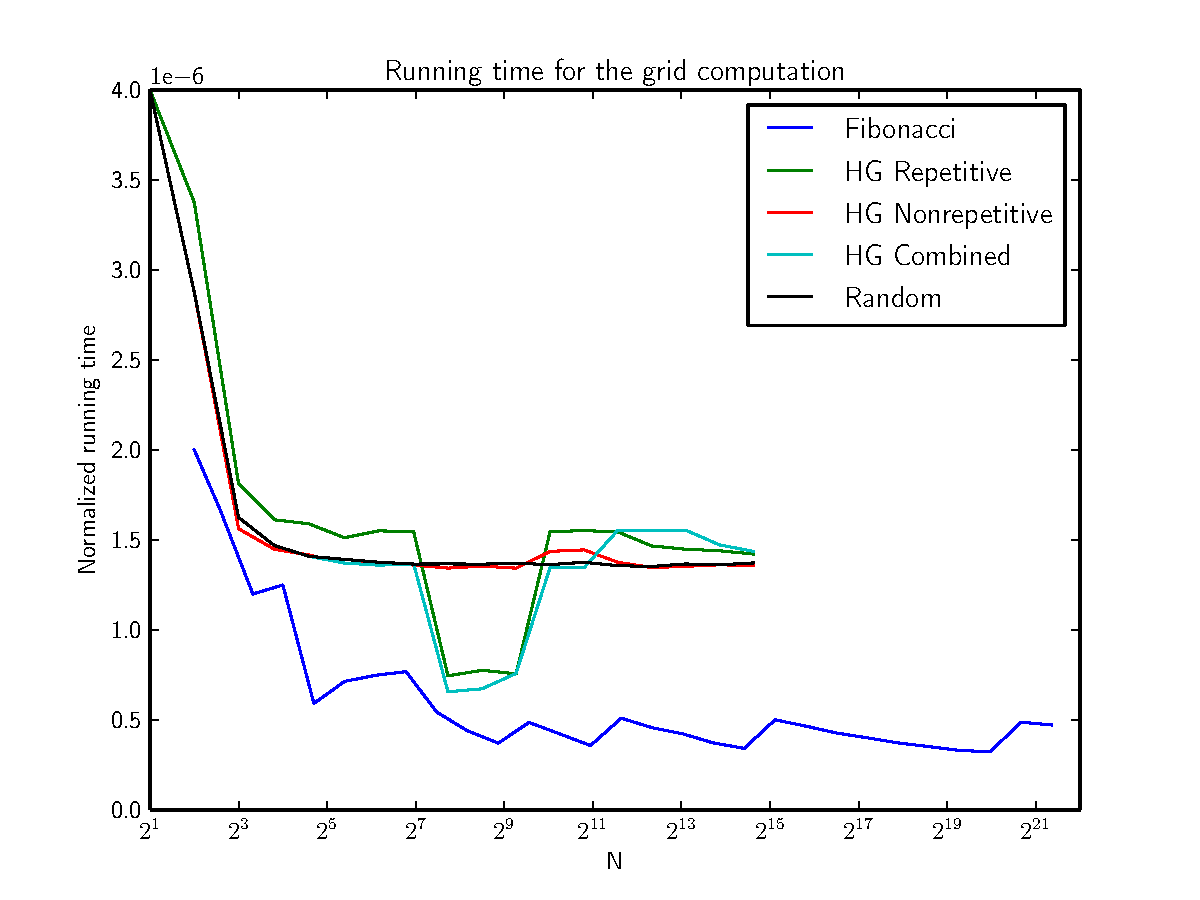
\includegraphics[width=10cm]{combined/grid_runningtime}
  \caption{Plot of the normalized running time for filling out the grid.}
  \label{fig:benchmark:fill-grid-time}
\end{figure}

% \begin{figure}[!htb]
%   \centering
%   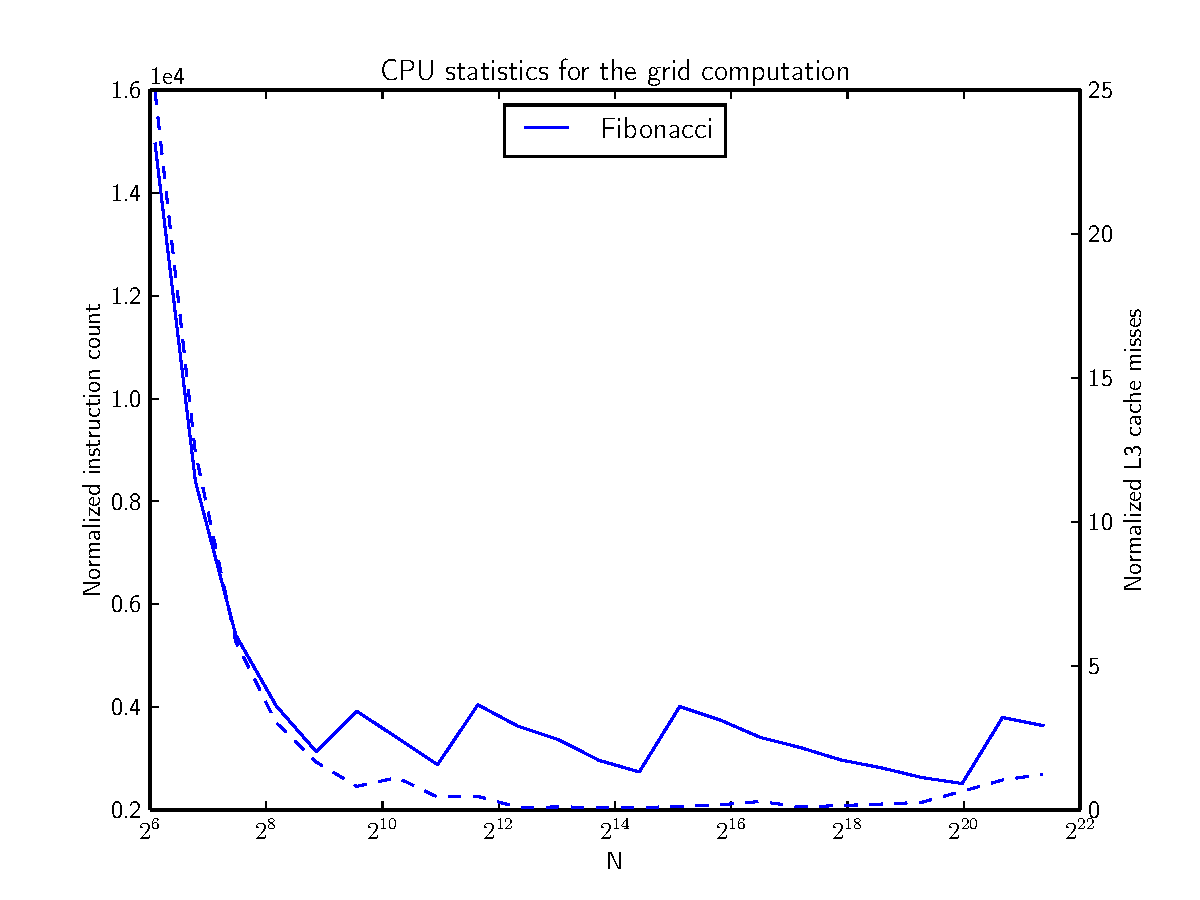
\includegraphics[width=10cm]{combined/grid_runningtime_cpu}
%   \caption{Plot of the normalized instruction count (solid line) and normalized L3 cache misses (dashed line) for filling out the grid with Fibonacci input.}
%   \label{fig:benchmark:fill-grid-cpu}
% \end{figure}

\clearpage
\subsubsection{Total combined running time}
This section will present measurements on the combined algorithm. First it will be verified that the theoretical running time is satisfied when all the steps are combined.

\Cref{fig:benchmark:total-time-combined} plots the normalized running time of the combined algorithm for the different inputs. The measurements indicates that the normalized running time for each type of input converges towards a constant.

It can be seen that the constant of the normalized running time for the random data and the non-repetitive human genome is substantially higher than for the Fibonacci input. This is believed to be the case because the block size of the algorithm depends on the compression ratio of the input, whereby input that has different compression characteristics may have different constants. There should be no input performing significantly worse than random strings, and hence it is concluded that the combined implementation seems to satisfy the theoretical running time bound from theory.
\begin{figure}[h!]
  \centering
  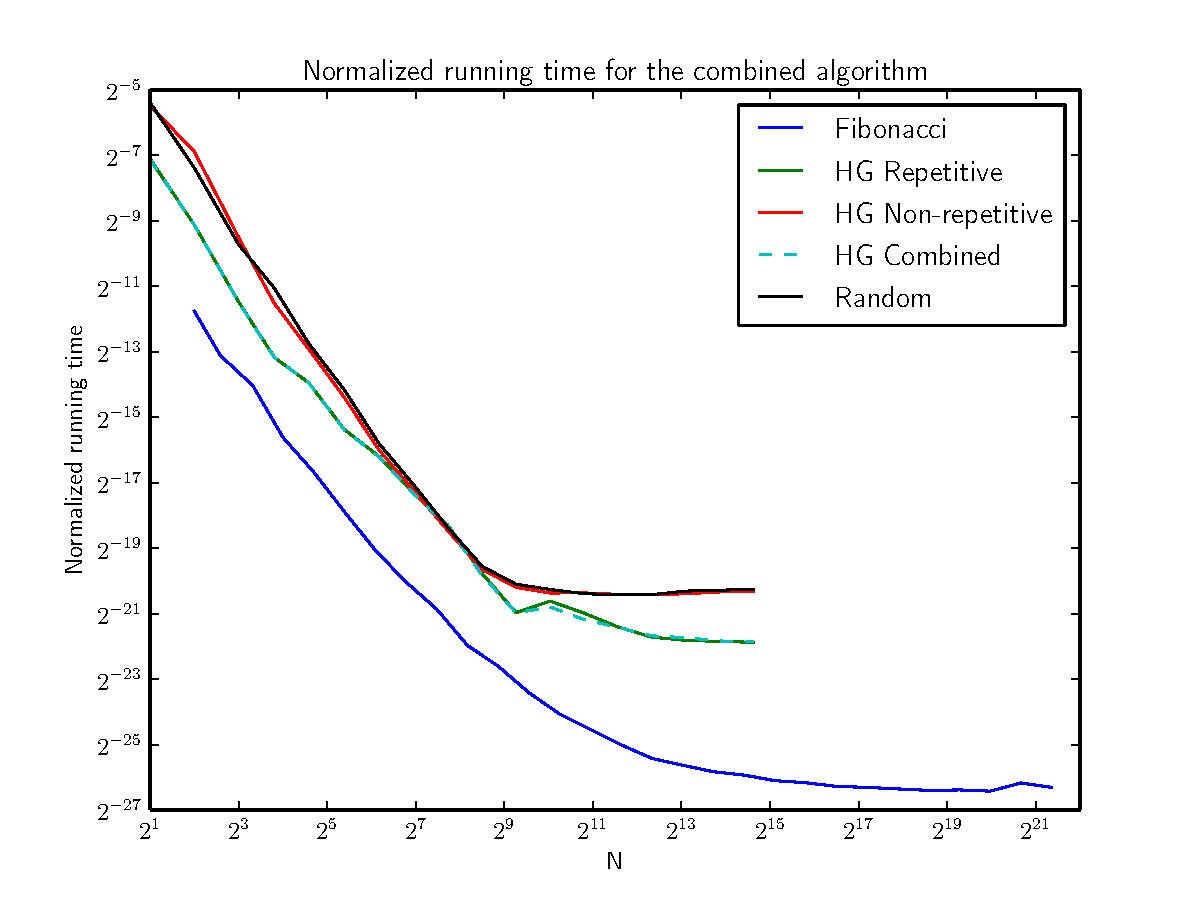
\includegraphics[width=13cm]{combined/total_runningtime}
  \caption{Plot of the normalized total running time of the combined algorithm.}
  \label{fig:benchmark:total-time-combined}
\end{figure}

\clearpage
\paragraph{Running time distribution}
It will now be examined how much of the running time is spend on the different parts of the algorithm for different input types and sizes. \Cref{fig:benchmark:relative-runningtime} shows how the relative time distribution is for the different input types.

It can be seen that the time for constructing and blocking the SLP takes almost all of the time for input sizes up to $\approx 2^9 = 512$. This is due to the high running time constant of building the suffix tree used to compute the LZ-factorization. However, as the input size gets larger, the relative time for computing the SLP gets negligible in the total running time. This is also what is predicted by the theoretical running times.

For the Fibonacci input, it can be seen that the running time between the grid computation and the DIST repository construction is more or less balanced. This is opposed to other the three inputs (the human genome combinations and the random string) where almost all the time is spend by the grid computation.

The time distribution is a result of the choice of the $\ffactor$ and $\xfactor$ from \cref{sec:benchmark:slp-partition-factors}. An interesting observation is that for random and human genome inputs the partition size is in the interval $[2, 3]$. This is the same block size giving the optimal running time for the Four Russian algorithm \cite{LasseFourRussian}. It was also found in \cite{LasseFourRussian} that the Four Russian algorithm used almost all the time filling out the grid. This indicates that the Four Russian algorithm will be a better choice for aligning these types of data, since the Four Russian algorithm uses a simpler algorithm for using the precomputed blocks.

Because Fibonacci inputs compress better the longer the input is, the partition size is increasing with the input size for the Fibonacci input. This is also why relatively the $\DIST$ repository computation takes up longer time for the Fibonacci input.

\newgeometry{left=1cm,right=1cm}
\begin{figure}[!ht]
  \centering
  \begin{subfigure}{0.495\textwidth}
    \centering
    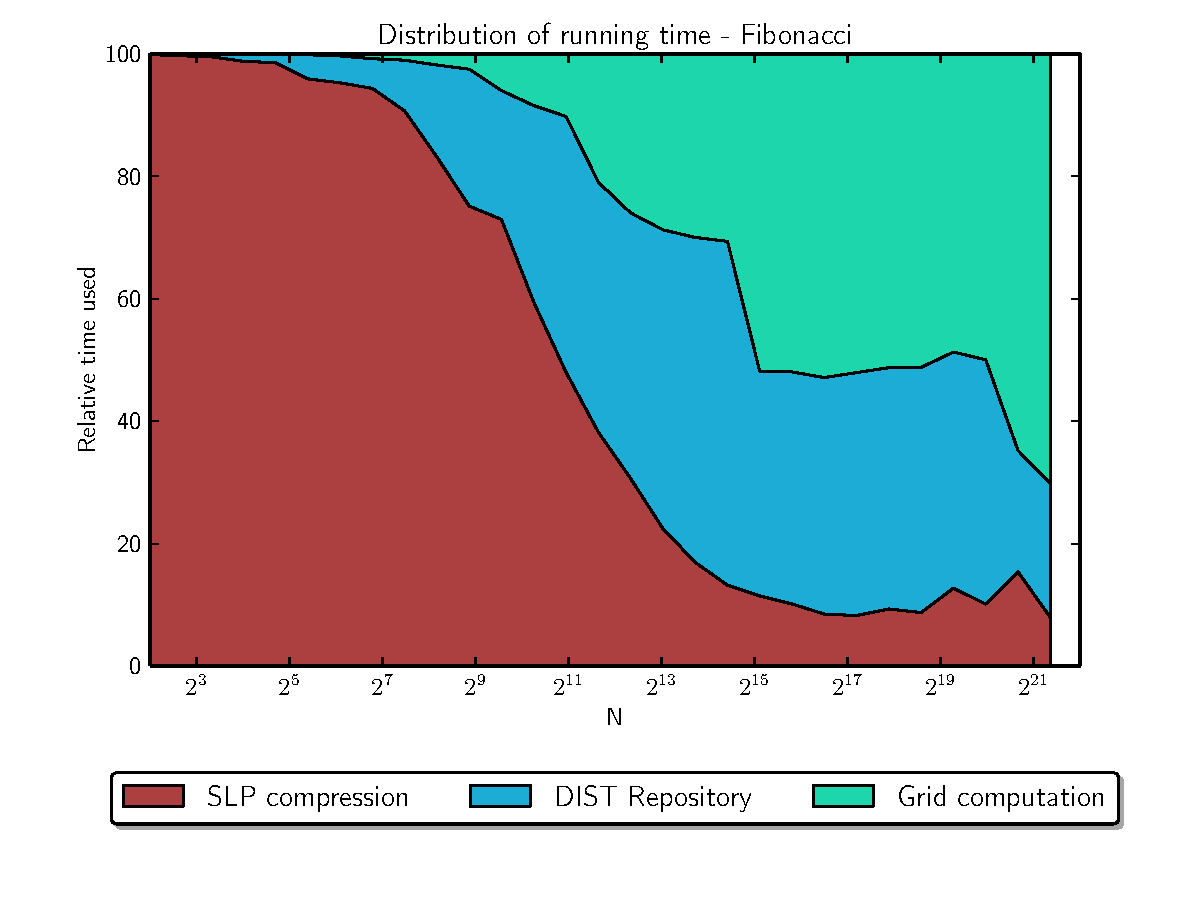
\includegraphics[width=\textwidth]{combined/fib_area_plot}
    \caption{Fibonacci input}
    \label{fig:benchmark:relative-runningtime-fib}
  \end{subfigure}
  %
  \begin{subfigure}{0.495\textwidth}
    \centering
    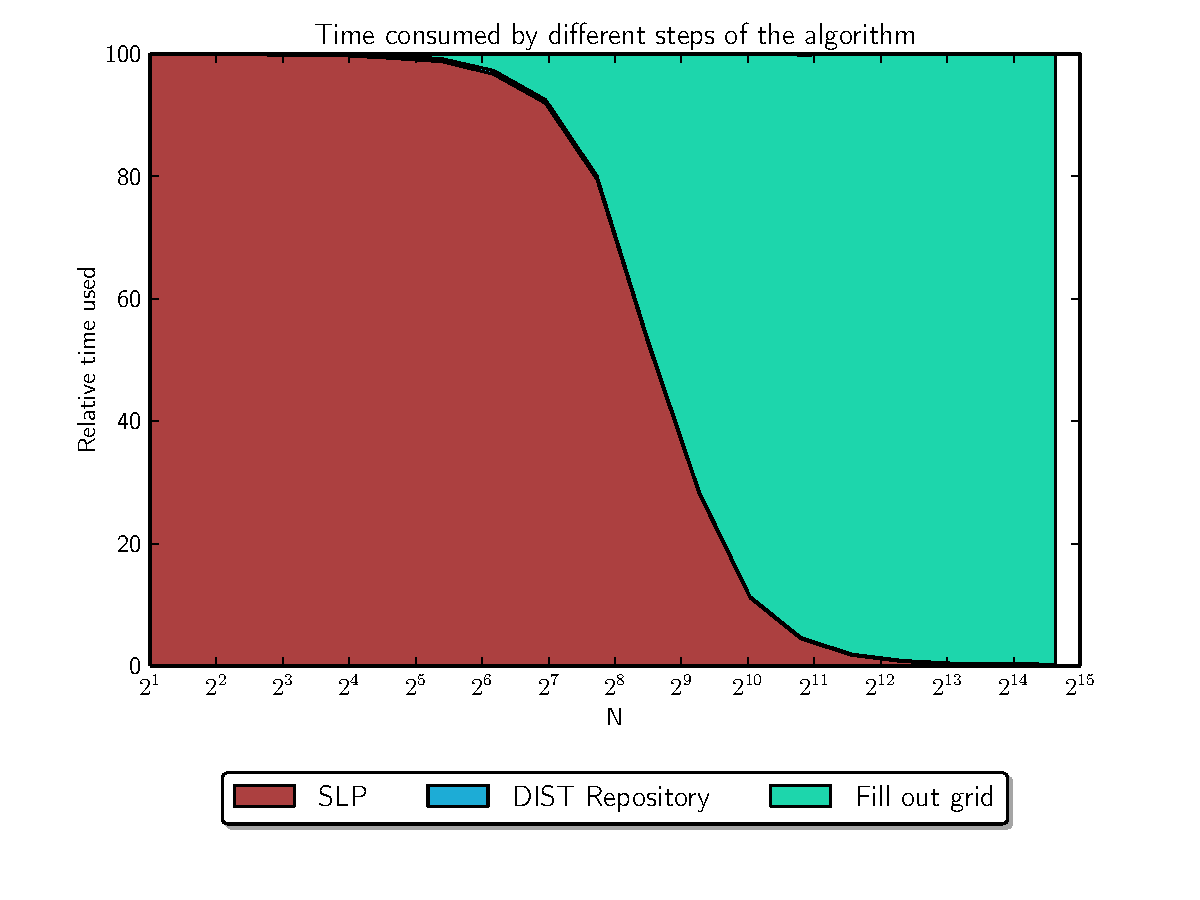
\includegraphics[width=\textwidth]{combined/random_area_plot}
    \caption{Random input}
    \label{fig:benchmark:relative-runningtime-random}
  \end{subfigure}

  \begin{subfigure}{0.495\textwidth}
    \centering
    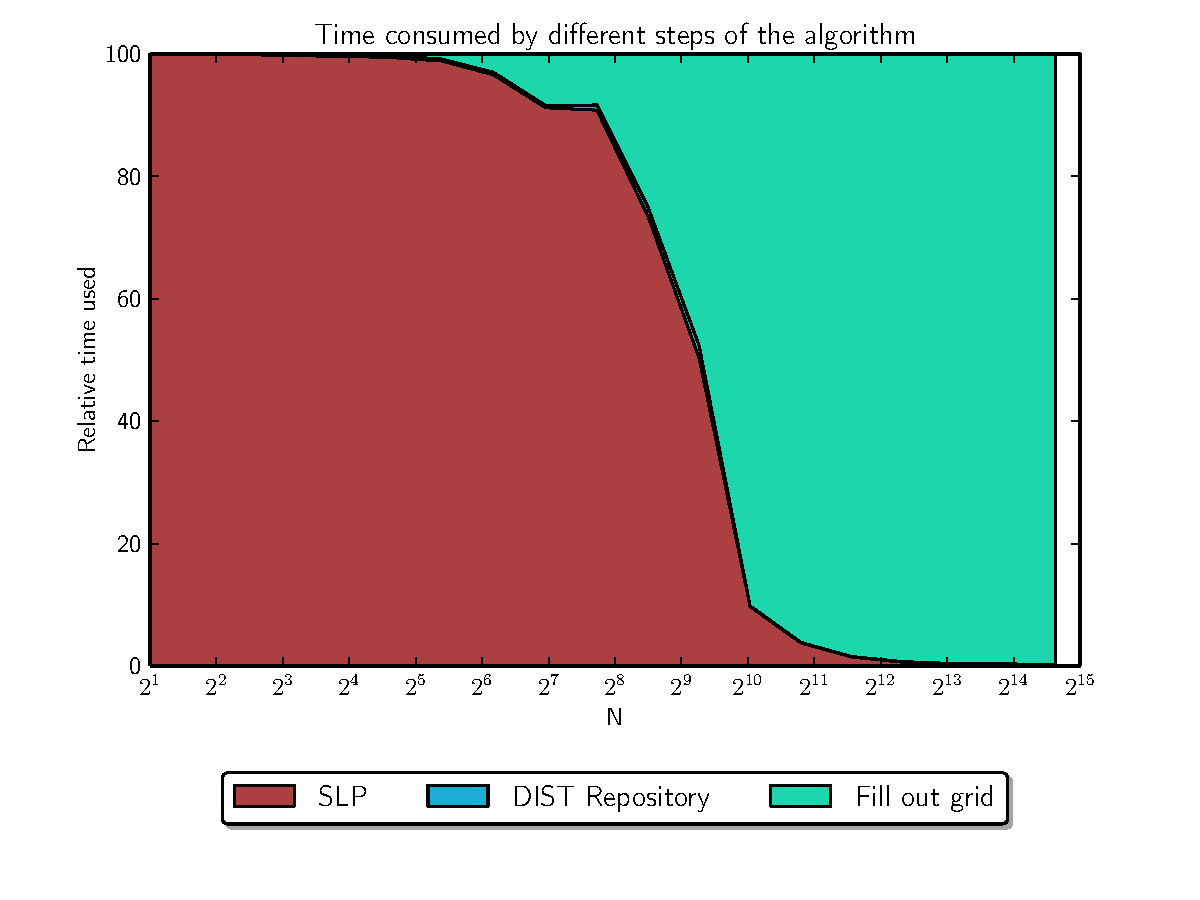
\includegraphics[width=\textwidth]{combined/hg_repetitive_area_plot}
    \caption{HG Repetitive / HG Combined}
    \label{fig:benchmark:relative-runningtime-hg-repetitive}
  \end{subfigure}
  %
  \begin{subfigure}{0.495\textwidth}
    \centering
    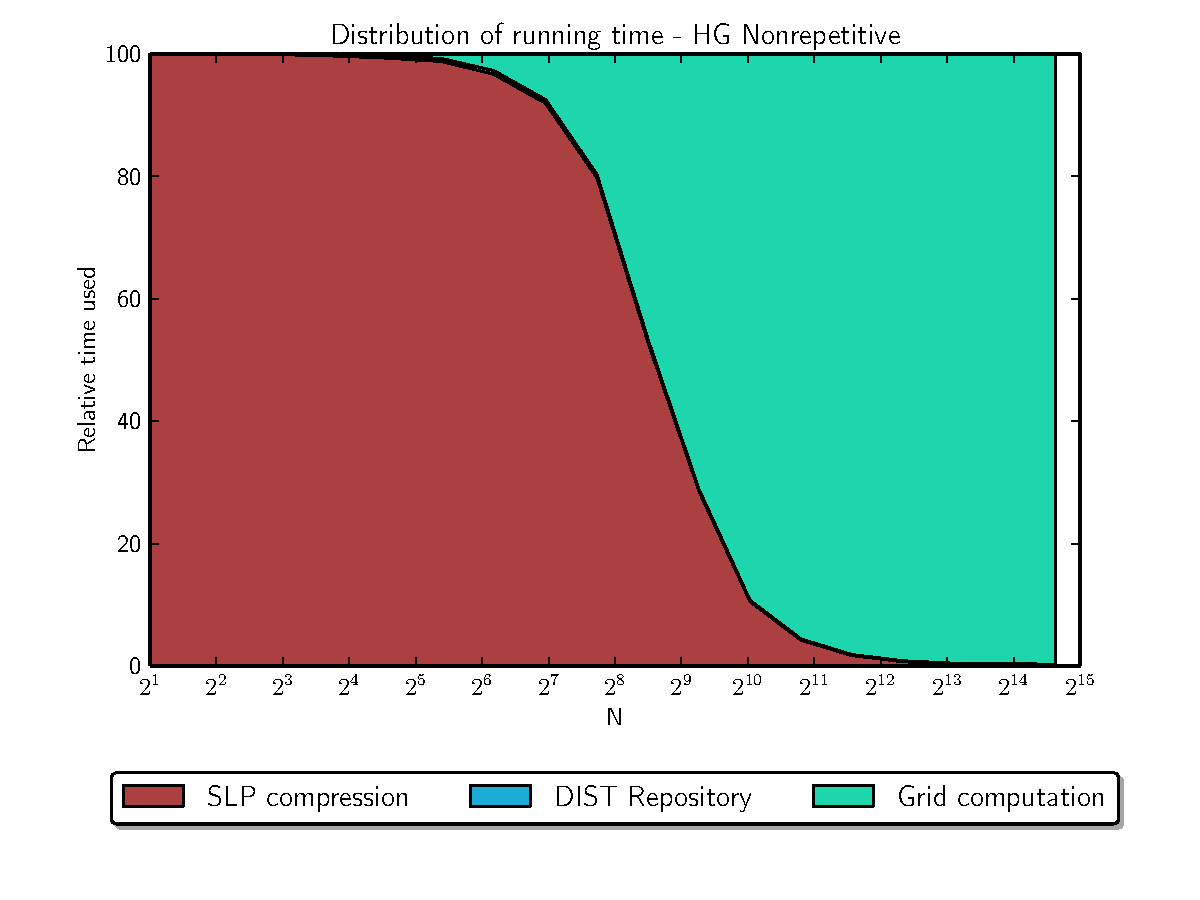
\includegraphics[width=\textwidth]{combined/hg_nonrepetitive_area_plot}
    \caption{HG Non-repetitive}
    \label{fig:benchmark:relative-runningtime-hg-nonrepetitive}
  \end{subfigure}
  \caption{Relative time consumption for the different steps of the algorithm.}
  \label{fig:benchmark:relative-runningtime}
\end{figure}
\restoregeometry

\clearpage
\subsubsection{Comparison with simple algorithms}
This section will present measurements on how the compression based algorithm performs compared to the simple algorithm. \Cref{fig:benchmark:simple-vs-lcsblowup} plots the speedup factor obtained over the simple algorithm for the different inputs.

For all the human genome inputs and the random inputs it can be seen that the algorithm performs $\approx 2^{8} = 256$ times slow than the simple algorithm. This is a quite disappointing result from the perspective of using the algorithm for DNA alignment and comparison. One natural thought is if there is something in the code that is directly responsible for the large slow down, but no such areas in the code was found by profiling. It is probably the case that some parts of the implementation can be optimized\footnote{Possible optimizations include double-dispatching without dynamic casts and better memory control.}. However, these optimizations should not be able to speed up the computation nowhere near the measured slowdown.

Since the alphabet is finite, the input strings can in theory be made to compress arbitrarily well by making the strings sufficiently long. The rate of this compression happens by a factor of $\Omega(\log_{|\Gamma|}{N})$ whereby the running time of the combined algorithm for all strings should be bounded by $O\left( N^2 \frac{\sqrt{\log{\log{N}}}}{\log{N}} \right)$. Because $\log{N}$ grows quite slow and the tremendous overhead in the compressed edit distance algorithm, the compression based algorithm will never be better than the simple algorithm for practical sized inputs that does not compress well under the SLP compression scheme.

It is also worth noticing that the simple algorithm may be improved. \cite{LasseFourRussian} experimented with the Four Russian algorithm for sequence alignment and found a speedup factor of $\approx 6-8$. Therefore the algorithm implemented in this thesis is not feasible for use in DNA sequence alignment.

The situation is different for Fibonacci inputs, which by \cref{sec:compression:benchmarks} is compressed such that $n = O(\log^2{N})$. This means that the total running time of the algorithm for Fibonacci input becomes $O\left( N\log^2{N} \sqrt{\log{\frac{N}{\log^2{N}}}} \right) = O(N\log^{\frac{5}{2}}{N})$. Therefore the running time of the compression based algorithm should improve by a factor $\Omega\left( \frac{N}{\log^{\frac{5}{2}}{N}} \right)$ over the simple algorithm.

It can be seen on \cref{fig:benchmark:simple-vs-lcsblowup-fib} that the actual speed-up factor seems to conform to theory. The actual speed-up in fact seems to be a bit better than the expression in the theoretical bound. The reason for the better asymptotic performance can mainly be explained by the $n = O(\log^2{N})$ SLP compression bound for the Fibonacci input contains some slack.

However, from \cref{fig:benchmark:simple-vs-lcsblowup} it can be seen that the length of the Fibonacci input should be longer than $\approx 2^{15} \approx 30000$ in order for the SLP-based algorithm to be faster than the simple edit-distance algorithm.

The benchmarks suggests that the algorithm is able to achieve a speedup in the edit distance computation for highly repetitive strings. However, in order to actually see any speedup the strings should be long. Moreover, it may be hard to think of practical input data that fulfill the highly repetitive structure. Therefore, the simple algorithm will for almost any practical purpose be a better choice.
\enlargethispage{\baselineskip}

\begin{figure}[!htb]
  \centering
  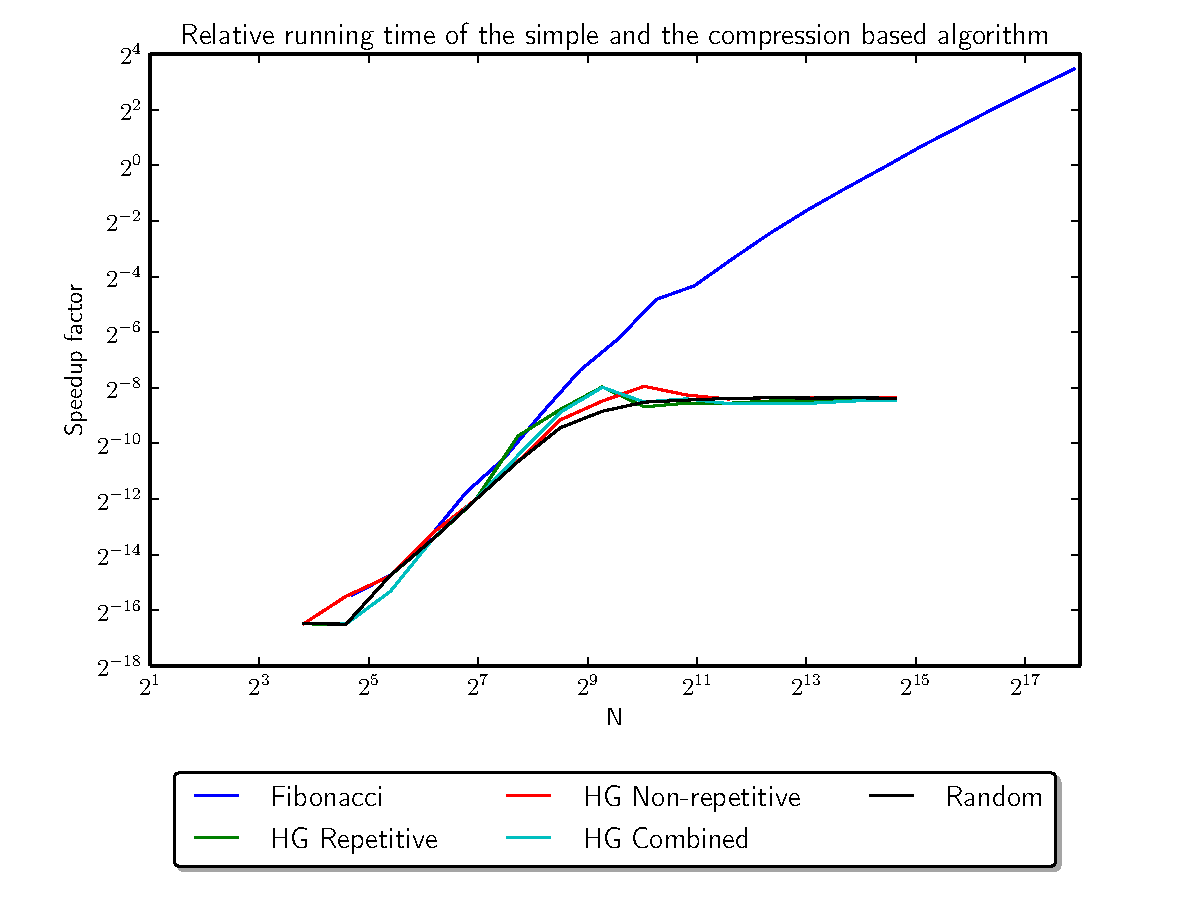
\includegraphics[width=10cm]{combined/simple_vs_lcs}
  \caption{Plot of the running time improvement of the compression based algorithm compared to the Simple algorithm.}
  \label{fig:benchmark:simple-vs-lcsblowup}
\end{figure}

\begin{figure}[!htb]
  \centering
  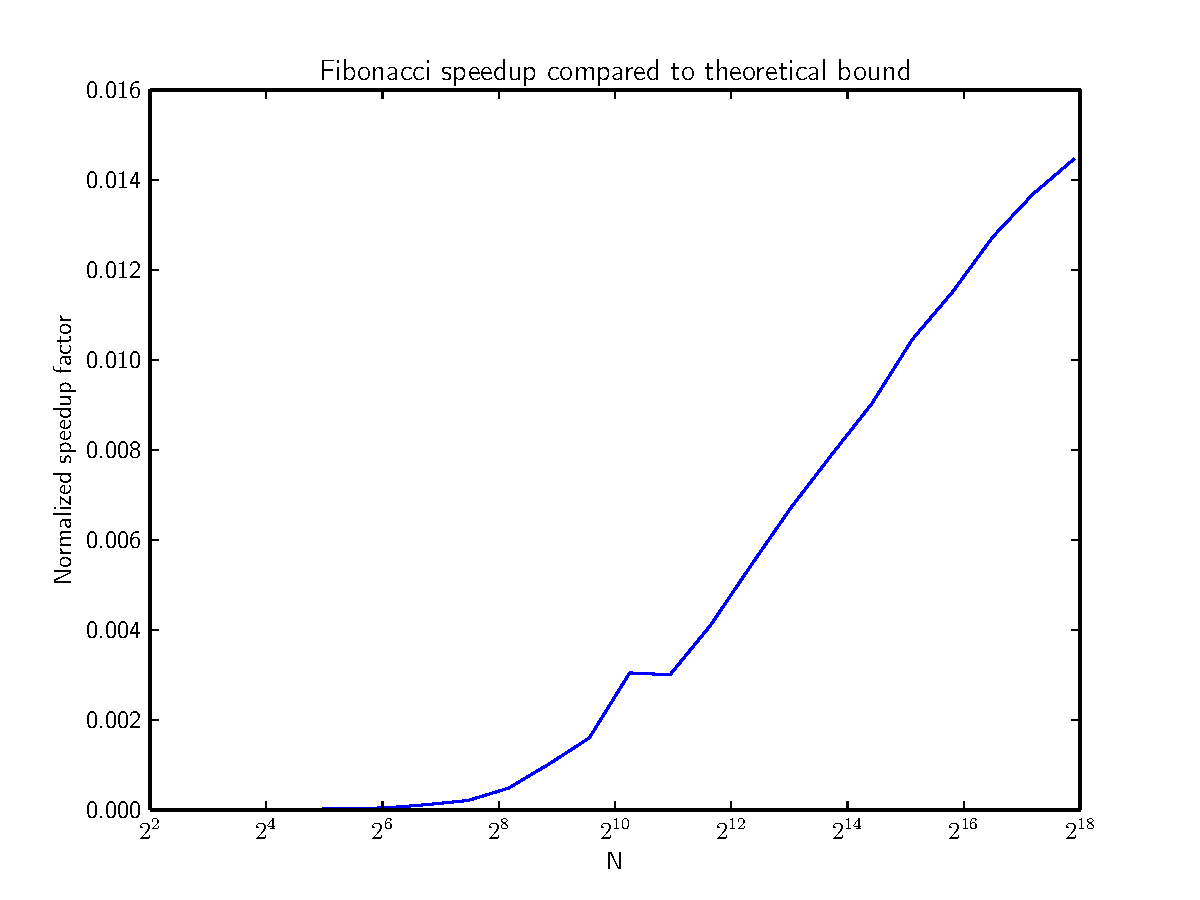
\includegraphics[width=10cm]{combined/simple-vs-lcs-fib}
  \caption{Comparison of the actual speed-up factor versus the theoretical speed-up factor for Fibonacci input.}
  \label{fig:benchmark:simple-vs-lcsblowup-fib}
\end{figure}

\chapter{Conclusion}
\label{chapter:conclusion}
During the work with this thesis, the algorithm for computing the Edit Distance described in \cite{Gawrychowski:2012:FAC:2422024.2422048} has been described, implemented and tested in practice.

The compression to SLPs of the input strings provides the foundation for obtaining a speedup. For the Fibonacci input, the inputs can automatically be compressed to a size of $O(\log^2{n})$ where the original input size is $n$. This results in an asymptotic improvement by a factor of $\Omega\left( \frac{N}{\log^{\frac{5}{2}}{N}} \right)$ for the theoretical running time of the compression based algorithm over the simple algorithm.

For the human genome and the random input, they obtain a compression to something above $0.2N$ for all tested input sizes, which was tested up to $\approx 4\cdot 10^6$ symbols. Therefore, for all practical applications, the algorithm on such input data has a theoretical running no better than the simple algorithm. Therefore all benchmarks with the human genome and random input the competition in practice becomes a battle on constants.

The running time of the algorithm when testing on Fibonacci input was found to be faster than the simple algorithm, when the input was longer than $\approx 30000$ symbols. This shows that there exist classes of inputs that does give a speedup in practice. However, it has not been possible to find any real world problems where the edit distance between such highly repetitive strings is desirable.

More practical input data is represented by the human genome. The human genome performed much the same way as a random string in the algorithm. For both types of input the compression based algorithm was found to be a factor of $\approx 256$ slower than the simple algorithm. This indicates that the practical applications of the compression based algorithm in its current form are very limited.

Another important thing to notice, is that the code for the compression based algorithm is immensely more complicated than the code for the simple algorithm. Also the Four Russian approach briefly described in \cref{sec:4-russian} is significantly less extensive to understand and implement.

Therefore the algorithm in its current form is not practical, as the simple algorithm or the Four Russian algorithm is superior except for very long inputs when computing on highly structured strings. However, it may be possible to improve the practicality of the algorithm so it can compete with the simple algorithm. Some ideas in order to improve the practicality of the algorithm is given in the following section.

\section{Future work}
\label{sec:conclusion:future-work}
During the project, a number of ideas (of which most are of practical concerns) for potentially improving the approach of computing the edit distance based on SLPs have been considered. These ideas are shortly described and motivated in the following list:

\begin{itemize}
  \item The algorithm for computing the minimum distance product of two unit-Monge matrices runs in time $O(n \log{n})$, however no lower bound other than $\Omega(n)$ is known. It could be interesting to close this gap. If is is possible to make a $\Theta(n)$ algorithm, the time for building the DIST tables can be reduced to $O(n^2 x)$, and by picking $x = \frac{N}{n}$, the total running time of the algorithm becomes $O(\underbrace{n^2 x}_{\DIST} + \underbrace{\frac{N^2}{x}}_{\text{Grid}}) = O(nN)$, which is an asymptotic improvement.

  \item Consider if the compressed strings can be reused, such that multiple strings can be entangled into one SLP. This would make it possible for a lot of strings to share DIST tables, and also possible do a better compression of highly similar strings. This could be of interest when computing the edit distance between all pairs of a large number of sequences, which is useful when approximating a phylogeny from sequence data.

  \item As mentioned in \cref{ch:compressing-strings}, the space consumption of the SLP has a very high constant when measured in terms of the number of productions in the SLP. As previously noted, this will mean that the approach is not applicable to long strings not compressing well. For the measurements performed in this thesis it did not turn out as a problem, however a succinct representation of a SLP may be of interest if it is possible to improve the running time of the algorithm.

  \item Another more direct way of obtaining a speedup is to parallelize the algorithm. The two SLP representations can easily be computed in parallel. Inside the construction of the SLPs the parallelization is not obvious, however, it was found in the benchmarks that this part only contribute a small fraction of the running time. Therefore the lack of parallelization in this step will not be a problem.

  For the expensive parts of the algorithm (constructing the DISTs and filling the dynamical programming grid), efficient parallelization is easy. For construction of the DIST repository, parallelization can be applied on every recursive merge, which happens for every pair of selected SLP productions and every recursive call.
  For filling out the grid, the algorithm can be parallelized in the same way as the simple algorithm, by choosing a suitable order to fill out the blocks.
\end{itemize}

%%%%%%%%%%%%%%%%%%%%%%%%%%%%%%%%%%%%%%%%%%%%%%%%%%%%%%%%%%%%%%%%%%%%%%%

\addcontentsline{toc}{chapter}{Bibliography}
\bibliographystyle{plain} 
\bibliography{refs}
%\addcontentsline{toc}{chapter}{Secondary Bibliography}
%\bibliographystyleB{plain} 
%\bibliographyB{refs} % remove this if you don't need secondary literature

\end{document}

